\documentclass[lang=cn,10pt]{elegantbook}
% 调用宏包
\usepackage{longtable}
\usepackage{multirow}
\usepackage{tabularx}
\usepackage{subcaption}
\usepackage{array}
\usepackage{pifont}
\usepackage{wrapfig}
\usepackage{ulem}
\usepackage{graphicx}
\usepackage{amsmath}
\usepackage{amssymb}
\usepackage{booktabs} % 用于三线表
\usepackage{geometry}


\doublespacing
\title{医学统计学「临床五年制」}
\subtitle{医学统计学 \LaTeX{} 教程}

\author{马鼎}
\bioinfo{编校}{董树磊}
\date{January 12, 2026}
\institute{白求恩第一临床医学院学业促进会}
\version{1.1}


\extrainfo{一切从现在开始都不晚。—— 栖川祯丞}

\setcounter{tocdepth}{3}

\logo{logo-xch.jpg}
\cover{cover.jpg}

% 本文档命令
\usepackage{array}
\newcommand{\ccr}[1]{\makecell{{\color{#1}\rule{1cm}{1cm}}}}

% 修改标题页的橙色带
\definecolor{customcolor}{RGB}{240,120,60}
\colorlet{coverlinecolor}{customcolor}

\begin{document}

\maketitle
\frontmatter

\tableofcontents

\mainmatter

\chapter*{前言} 
\markboth{前言}{前言} 

亲爱的同学：

见字如面。

当你翻开这份资料时，想必你也正在进行或刚刚结束了卫生学与流行病学那漫长而繁琐的记忆征途。如果说前面的章节是对记忆力的极限挑战，那么眼前的“医学统计学”，或许更像是一座需要逻辑与理性去攀登的高山。

这份资料主要面向临床医学五年制《预防医学》课程，基于2023级临床医学五年制授课PPT、预防医学教学大纲（2022版）、医学统计学（人民卫生出版社，第8版）编写。

我们深知，这是《预防医学》中唯一有非选择题的板块，也是让无数文理兼修的医学生感到“头秃”的重灾区。编写这份资料的初衷，源于编者自己备考时的切身体会。面对紧张的课时和较为单薄的数理基础，我也曾对着那一堆希腊字母和公式感到迷茫。因此，在这份笔记中，我们不仅梳理了授课的核心脉络，更将老师课件中的经典例题与我复习时的碎碎念一同收录其中。你会发现，这份资料里多了很多解题心路。这或许会让篇幅显得有些冗长，但请你海涵——因为我们希望当你陷入困惑时，这些笨拙的思考过程，能帮助你搭起跨越认知鸿沟的桥梁。

在此，也需要特别说明：本资料并不完全适用于 5+3 一体化等长学制的同学。长学制的《医学统计学》是一门独立且深邃的课程，其广度与难度远超《预防医学》中的统计学章节。因此，不建议长学制的同学将其作为复习的主力依据，但若将其作为理解基础概念的参考，或许也能带来些许启发。

在备考的最后阶段，请务必回归课堂，留意老师反复强调的那些能够“落地”的知识点。既然考场上不允许使用计算器，那么那些繁复的数字运算大概率不会出现。哪些适合作为大题考查手算与逻辑？哪些更适合在选择题中考察辨析？相信聪明的你，心中自有判断。统计学只是预防医学拼图中的一块。对于那些晦涩艰深的部分，不妨洒脱一些，抓大放小，方能游刃有余。

愿你落笔生花，不仅能顺利通过期末的考验，更能在这个数据驱动的医学时代，握紧通向真理的钥匙。

我们高处见。

\vspace{0.2cm}

 关于这份资料：

\begin{itemize}
    \item 它基于 \verb|Elegant Program| \LaTeX 模板编写。
    \item 它属于开放共享的星辰大海： 项目源码已托管于 GitHub，仓库之门在此敞开：\href{https://github.com/Mading706/Introduction-to-Medical-Research-and-Essay-Writing}{点点Star，支持一下$\sim$}
    \item 它由吉林大学白求恩第一临床医学院学业促进会悉心编校、严谨审核。但这绝非终点，我们温暖地在此发出邀请——期待你能接过接力棒，成为下一个执笔者，与我们一同修缮、维护，让这份互助的薪火生生不息。
\end{itemize}


\vspace{0.4cm}

前路漫漫，愿这点微光，能与你同行一程。

\hfill 编者 谨识

\hfill 2026年1月12日


\chapter{数值变量资料的统计描述}

\begin{introduction}
    \item 教学内容
    \begin{itemize}
        \item 集中趋势的描述
        \item 离散趋势的描述


    \end{itemize}
    \item 授课要点
    \begin{itemize}
        \item 集中趋势描述指标的定义、计算和适用条件
        \item 离散趋势描述指标的定义、计算和适用条件

    \end{itemize}
\end{introduction}

\section{集中趋势的描述}

\subsection{算术均数}

算术均数简称均数（mean）。总体均数用希腊字母 $\mu$ 表示，样本均数用 $\bar{X}$ 表示。适用于描述对称分布，尤其是正态分布或近似正态分布的数值变量资料的平均水平。计算方法有：

\subsubsection{直接法}
将所有观测值相加求和除以观测值个数。

\begin{equation}
\bar{X}=\frac{X_1+X_2+X_3+\cdots+X_n}{n}=\frac{\sum X}{n}
\end{equation}

式中 $\Sigma$ 是希腊字母，为求和符号。
\subsubsection{加权法}
适合于频数分布表资料求均数。

\begin{equation}
\bar{X}=\frac{f_1X_1+f_2X_2+f_3X_3+\cdots+f_kX_k}{f_1+f_2+f_3+\cdots+f_k}=\frac{\sum fX}{\sum f}=\frac{\sum fX}{n}
\end{equation}
\subsection{几何均数}

\subsubsection{直接法}
\begin{equation}
G=\sqrt[n]{x_1\cdot\cdots\cdot x_n}=\lg^{-1}\left(\frac{\lg x_1+\cdots+\lg x_n}{n}\right)=\lg^{-1}\left(\frac{\sum \lg x}{n}\right)
\end{equation}

\subsubsection{加权法}
\begin{equation}
G=\lg^{-1}\left(\frac{f_1\lg x_1+\cdots+f_k\lg x_k}{n}\right)
\end{equation}

\subsection{中位数}
\subsubsection{直接计算法}
\begin{equation}
M=\left\{\begin{array}{ll}
X_{\frac{n+1}{2}}, & n\text{为奇数}\\[6pt]
\frac{1}{2}\left(X_{\frac{n}{2}}+X_{\frac{n}{2}+1}\right), & n\text{为偶数}
\end{array}\right.
\end{equation}

\subsubsection{百分位数}

百分位数（$P_x$）是在一组数据中找到这样一个值，使得 $x\%$ 的观测值小于（或不大于）$P_x$，其余 $(100-x)\%$ 的观测值大于（或不小于）$P_x$。

对于分组资料（频数表），可用插值法估计：
\begin{equation}
P_x=L+\frac{i}{f}\left(n\cdot\frac{x}{100}-\sum f_L\right)
\end{equation}

\begin{itemize}
\item $L$ 为 $P_x$ 所在组段的下限；
\item $i$ 为该组段的组距；
\item $f$ 为该组段的频数；
\item $n$ 为样本含量；
\item $\sum f_L$ 为小于 $L$ 的各组段的累计频数。
\end{itemize}

\subsubsection{百分位数公式速记与避坑}

百分位数的插值公式常被视为难点，死记硬背容易出错。
\[
P_x = L + \frac{i}{f_x} \left( n \cdot x\% - \sum f_L \right)
\]

\paragraph{记忆心法：按比例插值（三步走）}

不要把公式看作一串符号，而是一个\textbf{“找人”}的过程。本质逻辑如下：

\begin{equation*}
    \text{结果} = \textbf{本组起点} + \textbf{组距} \times \underbrace{\frac{\text{还差几人}}{\text{本组总人数}}}_{\text{比例}}
\end{equation*}

\begin{enumerate}
    \item \textbf{确定起点 ($L$)}：
    目标落在哪一组？该组的\textbf{下限}就是起点。\\
    \textit{（相当于：我知道他在 70\textasciitilde80 分这一档，先把 70 分拿稳。）}

    \item \textbf{计算缺口 ($n \cdot x\% - \sum f_L$)}：
    目标名次减去\textbf{前一组}的累积人数。\\
    \textit{（相当于：我要找第 150 名，前一组累计到了 120 名，所以我还需要在这一组里数 30 个人。）}

    \item \textbf{按比例分配 ($\times \frac{i}{f_x}$)}：
    用缺口人数除以本组总人数，再乘以组距。\\
    \textit{（相当于：这 30 个人占本组 50 人的 $3/5$，所以分数也要往前走组距的 $3/5$。）}
\end{enumerate}

\paragraph{考场防坑指南}

\begin{description}
    \item[坑点一：$L$ 是下限 (Lower)]
    公式里的 $L$ 永远是所在组的\textbf{下限}，不是上限。因为我们是从小往大数的，是在“地板”的基础上往上加。

    \item[坑点二：$\sum f_L$ 看“前人”]
    这里的累积频数是指\textbf{目标组之前所有组}的合计，千万不要把本组的频数加进去，否则算出来的人就跑出这一组了。

    \item[坑点三：中间步骤不取整]
    计算位置指标 $n \cdot x\%$ 时，如果算出小数（例如 $15.75$），\textbf{绝对不要四舍五入}！直接把 $15.75$ 代入公式计算，这样结果才精确。
\end{description}

\subsubsection{频数表法（插值法）}
\begin{equation}
M=L+\frac{i}{f_M}\left(\frac{n}{2}-\sum f_L\right)
\end{equation}

\begin{itemize}
\item $L$ 为中位数所在组段的下限；
\item $i$ 为该组段的组距；
\item $f_M$ 为该组段的频数；
\item $\sum f_L$ 为小于 $L$ 的各组段的累计频数。
\end{itemize}

\vspace{0.2cm}

\begin{exercise}
    用频数表法计算中位数（表~\ref{tab:tg-630}）
\end{exercise}

\vspace{0.2cm}

\begin{solution}

样本含量 $n=630$，故 $\frac{n}{2}=315$。由累积频数可知：
\[27<196<315\le 363,\]

因此中位数所在组段为 $70\text{\textasciitilde}100$，取 $L=70$，组距 $i=30$，该组频数 $f_M=167$，且 $\sum f_L=196$。

\[M=70+\frac{30}{167}\left(315-196\right)\approx 91.4\,\mathrm{mg/dl}.\]

\end{solution}


\section{离散趋势的描述}
\subsection{全距}

全距又称极差，用 $R$ 表示：
\begin{equation}
R=X_{\max}-X_{\min}
\end{equation}

\subsection{四分位数间距}

四分位数（quartile）是特定的百分位数。第 25 百分位数（$P_{25}$）称为下四分位数，常用 $Q_L$ 表示；第 75 百分位数（$P_{75}$）称为上四分位数，常用 $Q_U$ 表示。四分位数间距（quartile interval）定义为：
\begin{equation}
IQR=Q_U-Q_L
\end{equation}

\subsection{方差}

方差（variance）是常用的变异指标。总体方差用 $\sigma^2$ 表示，样本方差用 $S^2$ 表示：
\begin{equation}
\sigma^2=\frac{\sum (X-\mu)^2}{N}
\end{equation}
\begin{equation}
S^2=\frac{\sum (X-\overline{X})^2}{n-1}
\end{equation}

\subsubsection{难点辨析：分母是 $N$ 还是 $n-1$？}

\begin{description}
    \item[总体标准差 ($\sigma$)] 分母为 $N$。
    \begin{itemize}
        \item \textbf{含义}：描述全部数据的真实波动。
        \item \textbf{理由}：已知总体均数 $\mu$，所有 $N$ 个数据均可自由变动，直接求平均即可。
    \end{itemize}
    
    \item[样本标准差 ($S$)] 分母为 $n-1$。
    \begin{itemize}
        \item \textbf{含义}：用样本估计总体的波动（无偏估计）。
        \item \textbf{理由 1 (自由度)}：计算 $S$ 时需先用样本均数 $\bar{X}$。一旦 $\bar{X}$ 确定，只有 $n-1$ 个数据能自由变动（损失 1 个自由度）。
        \item \textbf{理由 2 (贝塞尔校正)}：样本点总是聚集在样本均数 $\bar{X}$ 周围，导致分子 $\sum(X-\bar{X})^2$ 小于真实的 $\sum(X-\mu)^2$。为纠正这种\textbf{低估}，将分母缩小为 $n-1$ 以放大结果，使其逼近真实值。
    \end{itemize}
\end{description}

\subsection{标准差}

标准差（standard deviation）是方差的平方根。总体标准差用 $\sigma$ 表示，样本标准差用 $S$ 表示。计算公式为：
\begin{equation}
\sigma=\sqrt{\frac{\sum (X-\mu)^2}{N}}
\end{equation}

对于分组资料（频数表），常用加权计算样本标准差：
\begin{equation}
S=\sqrt{\frac{\sum fX^2-\frac{(\sum fX)^2}{n}}{n-1}}
\end{equation}

式中 $X$ 为各组段的组中值，$f$ 为相应的频数。

\vspace{0.2cm}

\begin{exercise}
    用频数表法计算样本标准差（表~\ref{tab:tg-630}）
\end{exercise}

\vspace{0.2cm}

\begin{solution}
由表~\ref{tab:tg-630} 可取各组段组中值分别为
$25,55,85,115,145,175,205,235,265,295,325$（组距均为 $30$），对应频数为
$27,169,167,94,81,42,28,14,4,3,1$，故样本量 $n=630$。

\[
\sum fX=27\times 25+169\times 55+\cdots+1\times 325=65370,
\]
\[
\sum fX^2=27\times 25^2+169\times 55^2+\cdots+1\times 325^2=8564550.
\]

代入频数表加权公式
\[
S=\sqrt{\frac{\sum fX^2-\frac{(\sum fX)^2}{n}}{n-1}}
=\sqrt{\frac{8564550-\frac{65370^2}{630}}{629}}
\approx 53.2\,\mathrm{mg/dl}.
\]
\end{solution}

\subsection{变异系数}

变异系数（coefficient of variation）常记为 $CV$，定义为标准差与均数之比：
\begin{equation}
CV=\frac{S}{\overline{X}}\times 100\%
\end{equation}

变异系数适用于比较度量衡单位不同的或均数相差悬殊的多组资料的变异程度。

\chapter{正态分布及其应用}

\begin{introduction}
    \item 教学内容
    \begin{itemize}
        \item 正态分布
        \item 正态分布的特征和曲线下面积分布规律
    \end{itemize}
    \item 授课要点
    \begin{itemize}
        \item 正态分布的概念
        \item 正态分布的基本特征
        \item 正态分布曲线面积的分布规律
    \end{itemize}
\end{introduction}

\section{正态分布的特征}

\begin{enumerate}
\item 正态曲线以均数为中心，左右对称。
\item 正态曲线的高峰位于均数所在处。
\item 正态分布具有 $\mu$（均值）与 $\sigma$（标准差）两个参数。
  $\mu$ 确定正态曲线的中心位置，$\mu$ 越大，曲线沿横轴越向右移动；反之越向左移动。
  $\sigma$ 确定曲线的形状，$\sigma$ 越大，曲线越扁平；$\sigma$ 越小，曲线越尖峭。
  一般用 $N(\mu,\sigma^2)$ 表示均数为 $\mu$、方差为 $\sigma^2$ 的正态分布。
\item 正态曲线下面积的分布有一定规律。
\end{enumerate}




\section{正态曲线下面积的分布规律}

对于 $X\sim N(\mu,\sigma^2)$，有下列常用区间概率（近似值）：
\begin{align*}
P(\mu-1\sigma<X<\mu+1\sigma) &\approx 68.27\%,\\
P(\mu-1.96\sigma<X<\mu+1.96\sigma) &\approx 95.00\%,\\
P(\mu-2.58\sigma<X<\mu+2.58\sigma) &\approx 99.00\%.
\end{align*}

\section{标准正态分布}

正态分布有两个不固定的参数 $\mu$ 与 $\sigma$。为了应用方便，可采取变量变换，使二者都为常数，即 $\mu=0$，$\sigma=1$。其变换为：
\begin{equation}
 u=\frac{x-\mu}{\sigma}
\end{equation}

此变换可把 $N(\mu,\sigma^2)$ 转化为 $\mu=0$、$\sigma=1$ 的正态分布 $N(0,1)$，称为\textbf{标准正态分布}（standard normal distribution）。

\vspace{0.2cm}
\begin{exercise}
    某生儿科考 85 分（班级 $\mu=80, \sigma=5$），外科考 75 分（班级 $\mu=60, \sigma=10$）。哪门课排名更好？
\end{exercise}

\vspace{0.2cm}
\begin{solution}
    \[ Z_{\text{儿}} = \frac{85 - 80}{5} = 1 \]
\[ Z_{\text{外}} = \frac{75 - 60}{10} = 1.5 \]

\textbf{结论}：$Z_{\text{外}} > Z_{\text{儿}}$，说明外科学成绩距离平均分更远（正向），相对排名更高。
\end{solution}


\vspace{0.2cm}
\begin{exercise}
已知红细胞 $\mu=4.8, \sigma=0.4$。问 $X=5.6$ 是否属于异常高值（$>97.5\%$ 人群）？
\end{exercise}

\vspace{0.2cm}
\begin{solution}
\[ Z = \frac{5.6 - 4.8}{0.4} = 2 \]

\textbf{结论}：因 $Z=2 > 1.96$（95\% 界值），说明该值位于正态曲线极右侧（$P < 0.025$），属于异常高值。
\end{solution}

\chapter{制定参考值范围}
\section{参考值范围的概念}

参考值范围（reference ranges）又被称为正常值范围，是指绝大多数正常人的解剖、生理、生化等各种数据的波动范围。


\section{参考值范围估计的基本步骤}

\begin{enumerate}
\item 从正常人的总体中进行随机抽样。
\item 对选定的正常人进行准确的测定。
\item 确定取单侧范围还是双侧范围。
\item 选择适当的百分范围。
\item 根据资料的分布类型选用恰当的估计方法。
\end{enumerate}

\section{参考值范围的估计方法}

根据资料的分布类型可选择正态分布法或百分位数法计算参考值范围。

\subsection{正态分布法}

正态分布法适用于正态分布或近似正态分布的资料。双侧 $100(1-\alpha)\%$ 参考值范围常用
\begin{equation}
\overline{X}\pm u_{\alpha/2}S
\end{equation}

其中 $u_{\alpha/2}$ 为标准正态分布上侧概率为 $\alpha/2$ 的分位数。

\vspace{0.2cm}
\begin{exercise}
    某地调查正常成年男子 144 人的红细胞数（近似正态分布），得均数为 $55.38\times 10^{12}/\mathrm{L}$，标准差为 $0.44\times 10^{12}/\mathrm{L}$。试估计该地成年男子红细胞数的 95\% 医学参考值范围。
\end{exercise}

\vspace{0.2cm}
\begin{solution}
红细胞数过多或过少均为异常，故应求双侧范围。取 $\alpha=0.05$，则 $u_{\alpha/2}=u_{0.025}=1.96$。

下限为：
\[
\overline{X}-u_{0.025}S=55.38-1.96\times 0.44=54.52\,(\times 10^{12}/\mathrm{L}),
\]

上限为：
\[
\overline{X}+u_{0.025}S=55.38+1.96\times 0.44=56.24\,(\times 10^{12}/\mathrm{L}).
\]

因此该地成年男子红细胞数的 95\% 医学参考值范围为 $\left(54.52,\,56.24\right)\times 10^{12}/\mathrm{L}$。
\end{solution}

\subsection{百分位数法}

百分位数法常用于偏态分布资料。以 95\% 参考值范围为例：
\begin{itemize}
\item 双侧：\ $\left(P_{2.5},\,P_{97.5}\right)$；
\item 单侧：\ $>P_{5}$ \ 或 \ $<P_{95}$。
\end{itemize}

\vspace{0.2cm}
\begin{exercise}
    用表~\ref{tab:tg-630} 的资料，采用百分位数法估计血清甘油三酯含量的 95\% 医学参考值范围。
\end{exercise}

\vspace{0.2cm}
\begin{solution}
样本量 $N=630$，组距 $h=30\,\mathrm{mg/dl}$。对分组资料，百分位数用线性插值：

\[
P_p=L+\frac{\left(pN-c\right)}{f}\,h,
\]

其中 $p$ 为所求分位点（如 0.025、0.975），$L$ 为所在组下限，$c$ 为该组前的累积频数，$f$ 为该组频数。

\begin{itemize}
\item $P_{2.5}$：$pN=0.025\times 630=15.75$，落在 $10\textasciitilde 40$ 组（$L=10$，$c=0$，$f=27$），

\[
P_{2.5}=10+\frac{15.75-0}{27}\times 30\approx 27.5\,\mathrm{mg/dl}.
\]

\item $P_{97.5}$：$pN=0.975\times 630=614.25$，落在 $220\textasciitilde 250$ 组（$L=220$，$c=608$，$f=14$），

\[
P_{97.5}=220+\frac{614.25-608}{14}\times 30\approx 233.4\,\mathrm{mg/dl}.
\]

\end{itemize}

因此该资料的 95\% 医学参考值范围为 $\left(27.5,\,233.4\right)\,\mathrm{mg/dl}$。
\end{solution}

\chapter{数值变量资料的统计推断}

\begin{introduction}
    \item 教学内容
    \begin{itemize}
        \item 总体均数的置信区间估计
    \end{itemize}
    \item 授课要点
    \begin{itemize}
        \item 均数的抽样误差的概念和注意事项
        \item 均数的标准误的定义、计算和意义
        \item t分布的概念、基本特征和应用
        \item 总体均数置信区间的方法、计算和应用条件
    \end{itemize}
\end{introduction}


\section{均数的抽样误差与标准误}

\subsection{均数的抽样误差}
样本均数与总体均数之差异，或各样本均数之间的差异，称为均数的抽样误差。

\subsection{标准误（standard error）}
反映均数抽样误差大小的指标是样本均数的标准差，简称标准误，记作 $\sigma_{\bar{x}}$ 或 $S_{\bar{x}}$。

\begin{equation}
S_{\bar{x}}=\frac{S}{\sqrt{n}}.
\end{equation}

\section{$t$ 分布}

\subsection{$t$ 分布的特征}
\begin{enumerate}
  \item $t$ 分布曲线以 $0$ 为中心，左右对称。
  \item $t$ 分布具有一个参数 $\nu$（称自由度，$\nu=n-1$）。$\nu$ 越小，曲线越扁平；$\nu$ 越大，曲线越接近标准正态分布；当 $\nu\to\infty$ 时，$t$ 分布趋近于标准正态分布。$t$ 分布是一簇曲线。
  \item $t$ 分布曲线下面积分布有一定规律。
\end{enumerate}

\subsection{$t$ 分布曲线下面积分布规律（即$t$ 界值表）}
\begin{figure}[htbp]
    \centering
    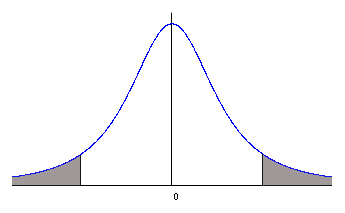
\includegraphics[width=0.75\linewidth]{image/t分布曲线下面积分布示意.png}
    \caption{t分布曲线下面积分布示意}
    \label{fig:t分布曲线下面积分布示意}
\end{figure}

\section{总体均数置信区间估计}
\subsection{概念}
根据样本均数，按给定的概率计算出总体均数很可能在的一个数值范围，这个范围称为总体均数的置信区间（confidence interval, CI）。

\subsection{方法}

\subsubsection{$u$ 分布法}

\begin{equation}
  \bar{x}\pm z_{\alpha/2}S_{\bar{x}}  
\end{equation}  

  适用条件：$\sigma$ 已知，或 $\sigma$ 未知但 $n$ 足够大。

\subsubsection{$t$ 分布法}

\begin{equation}
  \bar{x}\pm t_{\alpha/2,\,\nu}S_{\bar{x}}
\end{equation}  

  适用条件：$\sigma$ 未知，且 $n$ 较小（$\nu=n-1$）。

\section{医学参考值范围 VS 总体均数置信区间：用 $S$ 还是 $S_{\bar{x}}$？}

\begin{table}[htbp]
    \centering
    \caption{参考值范围 vs 置信区间 终极判别表}
    \begin{tabular}{p{2.5cm}p{5cm}p{5cm}}
        \toprule
        \textbf{比较维度} & \textbf{医学参考值范围} & \textbf{总体均数置信区间 (CI)} \\
        \midrule
        \textbf{核心问题} & “这个\textbf{病人}正常吗？” & “这个\textbf{平均数}准吗？” \\
        \textbf{关注对象} & \textbf{个体} (Individual) & \textbf{群体均值} (Parameter) \\
        \textbf{变异指标} & 标准差 \boldmath{$S$} & 标准误 \boldmath{$S_{\bar{x}} = S/\sqrt{n}$} \\
        \textbf{公式} & $\bar{X} \pm 1.96 \mathbf{S}$ & $\bar{X} \pm 1.96 \mathbf{S_{\bar{x}}}$ (或 $t_{\alpha/2} S_{\bar{x}}$) \\
        \textbf{样本量 $n$ 增大} & 范围\textbf{稳定} (人群差异不变) & 范围\textbf{变窄} (估计更精准) \\
        \bottomrule
    \end{tabular}
\end{table}

\section{总体均数 vs 样本均数}

\subsection{逻辑闭环图谱}

\begin{table}[htbp] %here, top, bottom
    \centering
    \caption{总体与样本的推断逻辑矩阵}
    \renewcommand{\arraystretch}{1.5} %间距扩大1.5倍
    \begin{tabular}{p{2.5cm}|p{5cm}|p{5cm}}
        \toprule
        \textbf{你的问题} & \textbf{你手里有总体参数 ($\mu, \sigma$)} & \textbf{你手里只有样本统计量 ($\bar{X}, S$)} \\
        \midrule
        \textbf{想看“个人”} & \textbf{直接描述} & \textbf{样本估算个体} \\
        (参考值范围) & $\mu \pm 1.96 \sigma$ & $\bar{X} \pm 1.96 \mathbf{S}$ \\
        \midrule
        \textbf{想看“总体”} & \textbf{无需估计} & \textbf{样本推断总体} \\
        (置信区间 CI) & $\mu$ 就是已知的，不用算区间！ & $\bar{X} \pm 1.96 \mathbf{S_{\bar{x}}}$ \\
         & & \small{(注意：这里要除以 $\sqrt{n}$)} \\
        \bottomrule
    \end{tabular}
\end{table}

\subsection{深度记忆：S 与 $S_{\bar{x}}$ 的本质分工}

\begin{description}
    \item[$\mathbf{S}$ (标准差)] \textbf{它是“散”的}。
    \begin{itemize}
        \item 它是衡量\textbf{个体}差异的。不管样本量 $n$ 多大，人与人的差异永远存在，所以 $S$ 不会变小。
        \item \textbf{应用}：计算医学参考值范围（判断某人是否正常）。
    \end{itemize}

    \item[$\mathbf{S_{\bar{x}}}$ (标准误)] \textbf{它是“准”的}。
    \begin{itemize}
        \item 它是衡量\textbf{均数}误差的。样本量 $n$ 越大，测得越准，误差越小，所以 $S_{\bar{x}} = S/\sqrt{n}$ 会随 $n$ 增大而趋近于 0。
        \item \textbf{应用}：计算置信区间（推断总体均数在哪里）、进行假设检验（$t$ 检验的分母）。~~
    \end{itemize}
\end{description}

\subsection{记忆口诀}

\begin{quote}
    \textbf{总体已知看分布，$\mu$ 加 $\sigma$ 框个人；}\\
    \textbf{样本入手分两路，看清题目问什么：}\\
    \textbf{问“病人”用 $S$，个体的差异不能缩；}\\
    \textbf{问“均数”用 $S_{\bar{x}}$，根号 $n$ 把误差磨。}
\end{quote}

\begin{quote}
    \textbf{病人看个休，波动 S 算；}\\
    \textbf{科研找均数，误差根号断 ($S/\sqrt{n}$)。}
\end{quote}


\chapter{数值变量资料的假设检验}

\begin{introduction}
    \item 教学内容
    \begin{itemize}
        \item 假设检验的基本思想和步骤
        \item t检验和Z检验
    \end{itemize}
    \item 授课要点
    \begin{itemize}
        \item 假设检验的基本思想
        \item 假设检验的基本步骤
        \item t检验的基本思想
        \item 单样本t检验基本思想、步骤和实例
        \item 配对设计的概念和特点
        \item 配对设计资t检验的基本思想、步骤和实例
        \item 假设检验应注意的问题

    \end{itemize}
\end{introduction}


\section{$t$ 检验和 $z$ 检验}

\subsection{$t$ 检验（$t$-test，Student's $t$-test）的应用条件}
当样本例数 $n$ 较小、样本来自正态总体、总体标准差 $\sigma$ 未知时，采用 $t$ 检验；
在做两个样本均数比较时，还要求两样本总体方差相等（方差齐性，homogeneity）。

\subsection{$z$ 检验（$z$-test）的应用条件}
主要适用于两样本含量 $n$ 较大（一般均大于 $50$）的情况。

\section{样本均数与总体均数的比较}

\subsection{单样本 $t$ 检验}
用于一组定量资料的样本均数 $\bar{x}$ 代表的未知总体均数 $\mu$ 与已知总体均数 $\mu_0$
（一般为理论值、标准值或经大量观察所得的稳定值）进行比较。

其检验统计量为
\begin{equation}
  t = \frac{\left|\bar{x}-\mu_0\right|}{S_{\bar{x}}} = \frac{\left|\bar{x}-\mu_0\right|}{S/\sqrt{n}}, \qquad \nu = n-1.
\end{equation}

\subsubsection{深度追问：$t$ 检验为什么除以 $S_{\bar{x}}$ 而不是 $S$？}

\begin{itemize}
    \item \textbf{1. 对象匹配（门当户对）}：
    分子是 $\bar{X} - \mu$（\textbf{均数}之差），分母必须是衡量\textbf{均数}波动程度的指标（即标准误 $S_{\bar{x}}$）。若用 $S$（个体波动），则是张冠李戴。
    
    \item \textbf{2. 样本量的力量}：
    $S_{\bar{x}} = S / \sqrt{n}$。
    \begin{itemize}
        \item 若用 $S$，样本量 $n$ 再大，$t$ 值也不变，无法体现大样本的优势。
        \item 用 $S_{\bar{x}}$，当 $n \uparrow \Rightarrow S_{\bar{x}} \downarrow \Rightarrow t \text{值} \uparrow \Rightarrow P \text{值} \downarrow$。这符合“样本量越大，越容易发现显著差异”的科学规律。
    \end{itemize}
    
    \item \textbf{3. 信号噪音比}：
    $t$ 检验衡量的是：\textit{“观察到的差异（信号）是抽样误差（噪音）的多少倍？”}
    \textbf{均数的抽样误差}只能用 $S_{\bar{x}}$ 表示。
\end{itemize}

\section{配对设计资料的比较}

\subsection{配对 $t$ 检验}

用于推断两种处理或处理前后的结果有无差别。利用差值 $d$ 的样本均数 $\bar{d}$
所代表的未知总体均数 $\mu_d$ 与已知总体均数 $\mu_{d0}$（常取 $\mu_{d0}=0$）进行比较。

其检验统计量为
\begin{equation}
  t = \frac{\left|\bar{d}-\mu_{d0}\right|}{S_{\bar{d}}} = \frac{\left|\bar{d}-0\right|}{S_d/\sqrt{n}} = \frac{\bar{d}}{S_d/\sqrt{n}}, \qquad \nu = n-1.
\end{equation}

式中各符号含义如下：
\begin{itemize}
  \item $d_i$：第 $i$ 对（或同一对象前后）观测值之差，常写作 $d_i=x_{i1}-x_{i2}$（例如“处理后$-$处理前”）。文中的 $d$ 表示差值这一随机变量；
  \item $\bar d$：差值的样本均数，$\bar d=\frac{1}{n}\sum_{i=1}^{n} d_i$；
  \item $\mu_d$：差值总体均数（未知参数），反映两种处理（或前后）在总体上的平均差异；
  \item $\mu_{d0}$：零假设 $H_0$ 下规定的差值总体均数（已知常数），通常取 $0$，即“总体平均差异为 0”；
  \item $S_d$：差值的样本标准差，$S_d=\sqrt{\frac{1}{n-1}\sum_{i=1}^{n}(d_i-\bar d)^2}$；
  \item $S_{\bar d}$：$\bar d$ 的标准误（standard error），$S_{\bar d}=\frac{S_d}{\sqrt{n}}$；
  \item $n$：配对数（即差值的样本量），等于可计算出 $d_i$ 的观测对数；
  \item $\nu$：自由度，$\nu=n-1$；
\end{itemize}

用于配对设计的定量资料的样本均数比较。配对设计主要有两种：
\begin{itemize}
  \item 同源配对（如同一对象处理前后，或同一对象接受两种不同处理）；
  \item 异源配对（如按某些条件配成对的不同对象）。
\end{itemize}

\vspace{0.2cm}
\begin{exercise}
    某护师随机抽取10名健康女大学生，在午饭后休息1小时，测试口腔温度，体温表分别在口腔中放置4分钟和7分钟，测试结果见表~\ref{tab:oral-temp-10}。试比较两种放置时间测试结果是否相同？
\end{exercise}

\vspace{0.2cm}
\begin{solution}
    本试验属于同源配对中两种不同的处理的比较。
    设差值 $d=\text{(7分钟)}-\text{(4分钟)}$，则检验假设为
    \[
      H_0: \mu_d=0, \qquad H_1: \mu_d\neq 0, \qquad \alpha=0.05.
    \]

    由表~\ref{tab:oral-temp-10} 得 $n=10$，$\sum d=2.05$，$\sum d^2=0.5475$，
    \[
      \bar d=\frac{\sum d}{n}=\frac{2.05}{10}=0.205,
    \]
    \[
      S_d=\sqrt{\frac{\sum d^2-(\sum d)^2/n}{n-1}}=
      \sqrt{\frac{0.5475-(2.05)^2/10}{10-1}}=0.1189.
    \]

    因而
    \[
      t=\frac{\bar d}{S_d/\sqrt{n}}=\frac{0.205}{0.1189}\sqrt{10}=5.45,\qquad \nu=n-1=9.
    \]

    查双侧临界值 $t_{\alpha,\nu}=t_{0.05,9}=2.262$。
    因 $|t|=5.45>2.262$，故 $P<0.05$，按 $\alpha=0.05$ 水准拒绝 $H_0$。
    认为两种放置时间的测试结果不相同，且 7 分钟测得的口腔温度高于 4 分钟。
    
\end{solution}

\section{两独立样本均数的比较}
两独立样本 $t$ 检验亦称成组 $t$ 检验，用于完全随机设计的定量资料的两样本均数的比较，
目的在于推断两样本均数各自所代表的总体均数 $\mu_1$ 和 $\mu_2$ 是否相等。
完全随机设计是指分别从两研究总体中随机抽取样本，然后比较两组的总体指标。

\subsection{两个大样本均数的比较}

\begin{equation}
  u=\frac{\left|\overline X_1-\overline X_2\right|}{S_{\overline X_1-\overline X_2}}
  =\frac{\left|\overline X_1-\overline X_2\right|}{\sqrt{\dfrac{S_1^2}{n_1}+\dfrac{S_2^2}{n_2}}}.    
\end{equation}


\begin{itemize}
    \item 大样本下，样本标准差 $S_1$ 和 $S_2$ 已经非常接近总体真实水平了，非常靠谱。
    \item 所以\textbf{不需要}费劲去搞“合并方差”了，直接各自算各自的标准误，然后合起来就行。
\end{itemize}

\subsection{两个小样本均数的比较}
\begin{equation}
  t=\frac{\left|\overline X_1-\overline X_2\right|}{S_{\overline X_1-\overline X_2}}
  =\frac{\left|\overline X_1-\overline X_2\right|}{\sqrt{S_c^2\left(\dfrac{1}{n_1}+\dfrac{1}{n_2}\right)}}
  =\frac{\left|\overline X_1-\overline X_2\right|}{\sqrt{\dfrac{(n_1-1)S_1^2+(n_2-1)S_2^2}{n_1+n_2-2}\left(\dfrac{1}{n_1}+\dfrac{1}{n_2}\right)}}.
\end{equation}

\[
  \nu=n_1+n_2-2.
\]

\begin{itemize}
    \item 为什么要算 $S_c^2$？
    \begin{itemize}
        \item 因为样本少，单独算甲组的 $S_1$ 和乙组的 $S_2$ 都不太准（波动大）。
        \item 既然假设两组方差是一样的（方差齐性），不如把两组的数据“混在一起”，算一个加权平均的方差，这样更稳、更准。
        \item 这个“混在一起”的方差就叫 合并方差 (Pooled Variance, $S_c^2$)。
    \end{itemize}
    \item 自由度的计算：
    $$\nu = n_1 + n_2 - 2$$
    （因为你算了两个均数 $\bar{X}_1$ 和 $\bar{X}_2$，消耗了 2 个自由度）。
\end{itemize}


\subsection{两独立样本比较：公式二选一}

在比较两组数据（如试验组 vs 对照组）的均数时，根据样本量大小选择不同公式。

\subsubsection{1. 小样本：成组 $t$ 检验 (Pooled $t$-test)}
\textbf{条件}：$n_1, n_2$ 较小 (通常 $\le 50$)，且方差齐。
\textbf{公式}：需计算合并方差 $S_c^2$。
\begin{equation}
    t = \frac{|\bar{X}_1 - \bar{X}_2|}{\sqrt{S_c^2 \left(\frac{1}{n_1} + \frac{1}{n_2}\right)}}, \quad \nu = n_1 + n_2 - 2
\end{equation}

其中合并方差：
\[ S_c^2 = \frac{(n_1-1)S_1^2 + (n_2-1)S_2^2}{n_1 + n_2 - 2} \]

\subsubsection{2. 大样本：成组 $u$ 检验 ($z$-test)}
\textbf{条件}：$n_1, n_2$ 较大 (通常 $> 50$)。
\textbf{公式}：无需合并，直接计算。
\begin{equation}
    u = \frac{|\bar{X}_1 - \bar{X}_2|}{\sqrt{\frac{S_1^2}{n_1} + \frac{S_2^2}{n_2}}}
\end{equation}

\textbf{判据}：计算出 $u$ 值后，直接与 \textbf{1.96} 比较。若 $|u| > 1.96$，则 $P < 0.05$。

\subsubsection{记忆口诀}

\section{统计推断底层逻辑解构}

统计推断的核心在于：我们如何从样本推测总体？

\subsection{路径一：上帝视角 ($Z$ 检验/$u$ 检验)}
如果我们处于理想世界，已知总体标准差 $\sigma$：
\begin{itemize}
    \item \textbf{理论基础}：样本均数 $\bar{X}$ 服从正态分布 $N(\mu, \sigma^2/n)$。
    \item \textbf{标准化}：
    \[ Z = \frac{\bar{X} - \mu}{\sigma/\sqrt{n}} \sim N(0,1) \]
    \item \textbf{判决标准}：查标准正态分布界值。
    \begin{itemize}
        \item 双侧 $\alpha=0.05$ 界值：\textbf{1.96}。
        \item 双侧 $\alpha=0.01$ 界值：\textbf{2.58}。
    \end{itemize}
\end{itemize}

\subsection{路径二：现实世界 ($t$ 检验)}
现实中 $\sigma$ 未知，只能用样本标准差 $S$ 代替：
\begin{itemize}
    \item \textbf{代价}：$S$ 本身也是估算的，存在波动。这种“不确定性”导致分布曲线“尾巴变厚、中间变矮”。
    \item \textbf{演变}：
    \[ t = \frac{\bar{X} - \mu}{S/\sqrt{n}} \sim t(\nu) \]
    \item \textbf{判决标准}：不再服从 $N(0,1)$，需查 $t$ 界值表，界值随自由度 $\nu = n-1$ 变化。
\end{itemize}

\section{关键公式的“为什么”}

\begin{enumerate}
    \item \textbf{为什么 $\sigma_{\bar{x}}^2 = \frac{\sigma^2}{n}$？}
    \begin{itemize}
        \item \textbf{直观理解}：平均值比单人值更稳定。样本量 $n$ 越大，均数的波动（方差）越小。
        \item \textbf{数学含义}：中心极限定理的推论。
    \end{itemize}
    
    \item \textbf{为什么 $S_{\bar{x}} = \frac{S}{\sqrt{n}}$？}
    \begin{itemize}
        \item 这是\textbf{标准误 (SE)}。
        \item \textbf{记忆口诀}：“胖瘦法则”。$S$ 描述个体（胖），$S_{\bar{x}}$ 描述均数（瘦）。想变瘦，必须除以 $\sqrt{n}$ 来“压惊”。
    \end{itemize}

    \item \textbf{为什么 $t$ 检验的分母是 $S_{\bar{x}}$？}
    \begin{itemize}
        \item 统计量的本质公式：
        \[ \text{统计量} = \frac{\text{信号 (观察值 - 理论值)}}{\text{噪音 (标准误)}} \]
    \end{itemize}
\end{enumerate}

\section{考场实战策略：大样本 vs 小样本}

考试中，样本量 $n$ 是决定解题速度的关键。

\subsection{量变引起质变}
当样本量 $n$ 足够大（通常 $n > 50$）时，样本标准差 $S$ 无限逼近总体标准差 $\sigma$，$t$ 分布无限逼近标准正态分布 ($Z$ 分布)。

\subsection{实战判别表}

\begin{table}[htbp]
    \centering
    \caption{小样本与大样本的考试处理策略}
    \begin{tabular}{lp{5cm}p{5cm}}
        \toprule
        \textbf{维度} & \textbf{小样本 ($n \le 50$)} & \textbf{大样本 ($n > 50$)} \\
        \midrule
        \textbf{标准差来源} & 样本标准差 $S$ & 样本标准差 $S$ \\
        \textbf{统计量符号} & $t$ 值 & $u$ 值 (近似 $Z$ 值) \\
        \textbf{判别界值} & \textbf{必须查 $t$ 界值表} & \textbf{固定为 1.96} ($\alpha=0.05$) \\
        \textbf{自由度} & 需关注 $\nu = n-1$ & 忽略 \\
        \textbf{解题心态} & 小心谨慎，防查错行 & \textbf{送分题，直接算} \\
        \bottomrule
    \end{tabular}
\end{table}

\subsection{大样本解题“三步走”}
\begin{itemize}
    \item \textbf{Step 1 确认}：看到 $n > 50$ (如 $n=100$)。
    \item \textbf{Step 2 计算}：
    \[ u = \frac{|\bar{X} - \mu_0|}{S/\sqrt{n}} \]
    \item \textbf{Step 3 判定}：
    \begin{itemize}
        \item 若 $|u| > 1.96$，则 $P < 0.05$，差异有统计学意义。
        \item 若 $|u| > 2.58$，则 $P < 0.01$，差异极显著。
    \end{itemize}
\end{itemize}




\chapter{分类变量资料的统计描述}

\begin{introduction}
    \item 教学内容
    \begin{itemize}
        \item 常用相对数
    \end{itemize}
    \item 授课要点
    \begin{itemize}
        \item 常用相对数的概念和意义
        \item 率、构成比和相对比

    \end{itemize}
\end{introduction}

常用相对数有：率、构成比和相对比。

\section{率}

率（rate）又称频率指标，说明某现象发生的频度或强度，常以百分率（\%）、千分率（\textperthousand）、万分率（1/万）、十万分率（1/10 万）等表示。计算公式为：

\begin{equation}
  \text{率}=\frac{\text{实际发生某现象的观察单位数}}{\text{可能发生某现象的观察单位总数}}\times K.
\end{equation}

其中，$K$ 为比例基数（如 100、1000、10000 等）。

\section{构成比}

构成比（proportion）又称构成指标，说明某事物内部某组成部分占其全部的比重或分布。计算公式为：

\begin{equation}
  \text{构成比}=\frac{\text{某事物内部某一部分的观察单位数}}{\text{某事物内部各部分的观察单位数总和}}\times 100\%.
\end{equation}

\section{相对比}

相对比（relative ratio）亦称比（ratio），指两个有关指标之比，说明两个指标的比例关系，常用倍数或百分数表示。计算公式为：

\begin{equation}
  \text{相对比}=\frac{\text{甲指标}}{\text{乙指标}}\,\,(\text{或}\times 100\%).   
\end{equation}

两个对比指标可以是绝对数、相对数或平均数等。例如，某地的男女性别比为绝对数之比；两地区某病死亡率之比为相对数之比；两地区 7 岁男童平均身高之比为平均数之比。




\chapter{分类变量资料的统计推断}

\begin{introduction}
    \item 教学内容
    \begin{itemize}
        \item 率的抽样误差和标准误
        \item 总体率的置信区间估计
    \end{itemize}
    \item 授课要点
    \begin{itemize}
        \item 率的抽样误差的概念和注意事项
        \item 率的标准误的定义、计算和意义
        \item 总体率置信区间的方法、计算和应用条件

    \end{itemize}
\end{introduction}

\section{率的抽样误差与标准误}

对于抽样研究，率和均数一样，也存在抽样误差，即伴随在抽样过程中的样本率与总体率之间的差异。同样，率的抽样误差的大小也用率的标准误来表示。

若总体率为 $\pi$，样本含量为 $n$，则样本率的总体标准误为：

\begin{equation}
  \sigma_p=\sqrt{\frac{\pi(1-\pi)}{n}}.
\end{equation}

实际工作中总体率 $\pi$ 往往未知，常用样本率 $p$ 代替，此时样本率的样本标准误为：

\begin{equation}
  S_p=\sqrt{\frac{p(1-p)}{n}}.
\end{equation}

\section{知识补丁：二项分布方差的直观理解}

对公式 $\sigma_p = \sqrt{\frac{\pi(1-\pi)}{n}}$ 感到困惑，其根源在于不理解二项分布的方差。

\subsection{1. 为什么方差跟 $\pi(1-\pi)$ 有关？}
想象抛硬币（或治疗病人），结果只有 0 和 1。
\begin{itemize}
    \item 当 $\pi=1$ 或 $\pi=0$ 时，结果确定，无波动，方差为 0。
    \item 当 $\pi=0.5$ 时，结果最不可测，波动最大。
\end{itemize}

数学式 $\pi(1-\pi)$ 恰好描述了这种\textbf{“两头为 0，中间最大”}的抛物线特性。

\subsection{2. 从总数到率的推导链}
\begin{enumerate}
    \item \textbf{单个人的方差}：$\sigma^2 = \pi(1-\pi)$
    \item \textbf{$n$ 个人的总方差}（二项分布）：因为个体独立，方差相加。
    \[ Var(X) = n \cdot \pi(1-\pi) \]
    \item \textbf{率 ($p=X/n$) 的方差}：常数 $1/n$ 提出来变平方。
    \[ Var(p) = \frac{Var(X)}{n^2} = \frac{n\pi(1-\pi)}{n^2} = \frac{\pi(1-\pi)}{n} \]
    \item \textbf{率的标准误}（开根号）：
    \[ \sigma_p = \sqrt{\frac{\pi(1-\pi)}{n}} \]
\end{enumerate}

\section{为什么率的标准误分母是 $n$？}

求连续变量标准差用 $n-1$，为什么求率的标准误用 $n$？

\begin{enumerate}
    \item \textbf{参数关系的本质不同}：
    \begin{itemize}
        \item \textbf{连续变量}：均数 ($\mu$) 和方差 ($\sigma^2$) 是\textbf{独立}的。估计方差时，因为借用了样本均数，损失了 1 个自由度，故需用 $n-1$ 校正。
        \item \textbf{二分类变量 (率)}：方差由均数 (率 $p$) \textbf{唯一决定} ($\sigma^2 = p(1-p)$)。只要有了 $p$，方差就确定了，无需进行独立的自由度校正。
    \end{itemize}

    \item \textbf{公式来源不同}：
    \begin{itemize}
        \item $S$ 来自对偏差平方和的\textbf{无偏估计}。
        \item $S_p$ 直接推导自二项分布方差公式 $Var(p) = Var(X/n) = \frac{np(1-p)}{n^2} = \frac{p(1-p)}{n}$。这里的 $n$ 是代数约分的结果。
    \end{itemize}
\end{enumerate}

\section{率的标准误：$\pi$ 与 $p$ }

\subsection{总体率的标准误 ($\sigma_p$)}
    \[ \sigma_p = \sqrt{\frac{\pi(1-\pi)}{n}} \]
    
    \textbf{适用}：已知总体率 $\pi$ 的理论推导（上帝视角）。

\subsection{样本率的标准误 ($S_p$)}
    \[ S_p = \sqrt{\frac{p(1-p)}{n}} \]
   
    \textbf{适用}：\textbf{实战专用}。当 $\pi$ 未知时，用样本率 $p$ 代替 $\pi$ 进行估算。
    
    \textbf{记忆}：\textbf{“成功率 $\times$ 失败率，除以 $n$，开根号。”}


\vspace{0.2cm}
\begin{exercise}
    某研究者抽样调查某地区三联疫苗接种者 500 人，接种后 35 名出现皮疹，发生率为 7\%，试计算率的标准误。
\end{exercise}

\vspace{0.2cm}
\begin{solution}
\[
  S_p=\sqrt{\frac{p(1-p)}{n}}=\sqrt{\frac{0.07(1-0.07)}{500}}=0.0114.
\] 
\end{solution}

\section{总体率的置信区间估计}

总体率（$\pi$）的估计包括点估计与区间估计。

\subsection{正态近似法}

当 $np$ 与 $n(1-p)$ 均大于 5 时，总体率（$\pi$）的 95\% 可信区间可取：

\begin{equation}
  \left(p-1.96S_p,\,p+1.96S_p\right).
\end{equation}

\subsection{查表法}

当 $n$ 较小（如 $n\le 50$），特别是 $p$ 接近于 0 或 1 时，宜采用查表法。

\vspace{0.2cm}
\begin{exercise}
为了解某药的疗效，对 100 名患者治疗的结果进行调查，结果为 80 人有效，有效率为 80\%。
\end{exercise}

\begin{solution}
\[
  S_p=\sqrt{\frac{p(1-p)}{n}}=\sqrt{\frac{0.80(1-0.80)}{100}}=0.04.
\]

该药有效率的 95\% 可信区间为：

\[
  \left(p-1.96S_p,\,p+1.96S_p\right)=\left(0.80-1.96\times 0.04,\,0.80+1.96\times 0.04\right)=(0.7216,\,0.8784).
\]

\end{solution}

\chapter{分类变量资料的统计分析}

\begin{introduction}
    \item 教学内容
    \begin{itemize}
        \item $\chi^2$检验


    \end{itemize}
    \item 授课要点
    \begin{itemize}
        \item $\chi^2$检验的基本思想
        \item 四格表资料$\chi^2$检验的基本思想、步骤和实例

    \end{itemize}
\end{introduction}
\section{四格表（$2\times 2$）资料的 $\chi^2$ 检验}

四格表资料常用于比较两组率（如有效率、阳性率等）。设两组分别为“对照组/试验组”，结局为“有效/无效”，实际频数（观察频数）记为：
\begin{center}
\begin{tabular}{cccc}
  \hline
  & 有效 & 无效 & 合计\\
  \hline
  对照组 & $a$ & $b$ & $a+b$\\
  试验组 & $c$ & $d$ & $c+d$\\
  合计 & $a+c$ & $b+d$ & $n=a+b+c+d$\\
  \hline
\end{tabular}
\end{center}

\subsection{基本思想}
原假设 $H_0$：两组总体率相同（等价于 ``分组'' 与 ``结局'' 相互独立）。

在 $H_0$ 成立时，各格的理论频数（期望频数）为

\[
  T_{ij}=\frac{n_{i+} \times n_{+j}}{n},\qquad (i=1,2;\,j=1,2),
\]

其中 $n_{i+}$、$n_{+j}$ 分别为第 $i$ 行与第 $j$ 列的边际合计数。

\subsection{深度理解：理论频数 $T$ (The "Should-Be" Value)}

公式：
$$T_{ij} = \frac{n_{i+} \times n_{+j}}{n}$$

\subsubsection{直观含义}
\textbf{理论频数 $T$} 是在 $H_0$ 假设（两变量\textbf{互不相干/独立}）成立的前提下，\textbf{理应出现}的数值。
\begin{quote}
    就像“分蛋糕”：如果大家胃口都一样（独立），那么每个人分到的蛋糕应该和全班的总比例一致。
\end{quote}

\subsubsection{公式的物理逻辑}
为什么是 $\frac{\text{行合计} \times \text{列合计}}{\text{总例数}}$？
这是一个\textbf{“总体概率投影”}的过程：
\begin{itemize}
    \item 全班的平均发生率 = $\frac{\text{列合计}}{n}$
    \item 某行的理论发生数 = 该行总人数 $\times$ 全班平均发生率
    \[ T = \text{行合计} \times \frac{\text{列合计}}{n} = \frac{\text{行} \times \text{列}}{n} \]
\end{itemize}

\subsubsection{理论频数在检验中的作用}
它是衡量\textbf{“扭曲程度”}的基准线。
\begin{itemize}
    \item 实际频数 $A$ 是现实；理论频数 $T$ 是理想。
    \item $\chi^2$ 统计量就是累加每一个格子 \textbf{“现实偏离理想”} 的程度（$(A-T)^2/T$）。偏离越大，说明变量间越可能有关系。
\end{itemize}

\subsection{$\chi^2$ 统计量}
比较实际频数 $A$ 与理论频数 $T$ 的偏离程度：

\begin{equation}
    \chi^2=\sum_{i=1}^{2}\sum_{j=1}^{2}\frac{(A_{ij}-T_{ij})^2}{T_{ij}}.
\end{equation}

若 $H_0$ 成立且样本量足够大，则 $\chi^2$ 近似服从自由度为

\begin{equation}
  \nu=(r-1)(c-1)=(2-1)(2-1)=1
\end{equation}

的卡方分布。

\subsubsection{卡方公式为什么要除以 $T$？}

公式：$\displaystyle \chi^2 = \sum \frac{(A-T)^2}{T}$

很多人只关注分子的平方差，却忽略了分母 $T$ 的关键作用。

\paragraph{消除“贫富差距”（相对化）}
\begin{itemize}
    \item \textbf{绝对误差的陷阱}：
    \begin{itemize}
        \item 10000 变成 10010（差 10），波动仅 0.1\%。
        \item 10 变成 20（差 10），波动高达 100\%。
    \end{itemize}
    若只看 $(A-T)^2$，两者的贡献一样（都是 100），这不公平。
    \item \textbf{除以 $T$ 的作用}：
    相当于衡量\textbf{“偏离率”}。让基数大的数据容忍度更高，基数小的数据容忍度更低。
\end{itemize}

\paragraph{数学本质（标准化）}

回顾 $Z$ 分数平方：$Z^2 = \frac{(X-\mu)^2}{\sigma^2}$。
在计数数据中，方差 $\sigma^2$ 近似等于均值（理论频数 $T$）。
\begin{quote}
    \textbf{结论}：除以 $T$，本质上就是\textbf{除以方差}。它是为了把绝对数值转化为\textbf{“标准差的倍数”}，从而实现不同量级数据的标准化累加。
\end{quote}

\subsection{$\chi^2$ 统计量适用条件提示}
一般要求各格理论频数不宜过小（常用经验：所有 $T_{ij}\ge 5$ 或至多 1 格 $T_{ij}<5$ 且无 $T_{ij}<1$）。当理论频数过小，可考虑连续性校正或 Fisher 确切概率法。

\subsection{判定}
给定显著性水平 $\alpha$：

\begin{itemize}
  \item 若 $\chi^2\ge \chi^2_{\alpha,\nu}$，则 $P\le \alpha$，拒绝 $H_0$（提示两组率有差异）；
  \item 若 $\chi^2< \chi^2_{\alpha,\nu}$，则 $P>\alpha$，不拒绝 $H_0$。
\end{itemize}

\subsection{四格表 $\chi^2$ 检验的专用公式}
对 $2\times 2$ 四格表，$\chi^2$ 统计量可化简为

\begin{equation}
  \chi^2=\frac{(ad-bc)^2\,n}{(a+b)(c+d)(a+c)(b+d)}.
\end{equation}

\subsection{连续性校正（Yates 校正）}
当理论频数偏小但仍可近似用 $\chi^2$ 分布时，可作连续性校正：

\begin{equation}
  \chi^2_c=\sum_{i=1}^{2}\sum_{j=1}^{2}\frac{\bigl(|A_{ij}-T_{ij}|-0.5\bigr)^2}{T_{ij}}
  =\frac{\bigl(|ad-bc|-n/2\bigr)^2\,n}{(a+b)(c+d)(a+c)(b+d)}.
\end{equation}

\subsection{四格表资料的Fisher确切概率法}
Fisher 确切概率法（Fisher's exact test）由 Ronald Fisher 于 1934 年提出，是一种基于超几何分布的检验方法，可在样本量较小或理论频数过小的情况下直接计算 $P$ 值。

\textbf{基本思想：}在四格表边缘合计数固定不变的条件下，计算四格表各种可能分配的概率 $P_i$，并据此求单侧或双侧累积概率 $P$，再与检验水准比较以判断是否拒绝 $H_0$。

对于四格表
\begin{center}
\begin{tabular}{cccc}
  \hline
  & 结局 1 & 结局 2 & 合计\\
  \hline
  组 1 & $a$ & $b$ & $a+b$\\
  组 2 & $c$ & $d$ & $c+d$\\
  \hline
  合计 & $a+c$ & $b+d$ & $n$\\
  \hline
\end{tabular}
\end{center}

在边缘合计数固定时，出现该表的概率为
\begin{equation}
  P_i=\frac{(a+b)!\,(c+d)!\,(a+c)!\,(b+d)!}{a!\,b!\,c!\,d!\,n!}.
\end{equation}

\subsection{四格表资料的经验适用规则}
对于四格表资料，通常可按下列经验规则选用方法：
\begin{enumerate}
  \item 当 $n\ge 40$ 且所有 $T_{ij}\ge 5$ 时，用 $\chi^2$ 检验的基本公式或四格表 $\chi^2$ 检验的专用公式；
  \item 当 $n\ge 40$，但存在 $1\le T_{ij}<5$ 时，用四格表 $\chi^2$ 检验的连续性校正公式；
  \item 当 $n<40$ 或存在 $T_{ij}<1$ 时，宜考虑 Fisher 确切概率法。
\end{enumerate}

\vspace{0.2cm}
\begin{exercise}
呋达帕胺片治疗原发性高血压疗效：将患者随机分为两组，试验组用呋达帕胺片加辅助治疗，对照组用安慰剂加辅助治疗。试分析试验组的有效率是否高于对照组。

\begin{table}[htbp]
\centering
\caption*{两种疗法治疗原发性高血压的疗效}
\begin{tabular}{ccccc}
  \hline
  组别 & 有效 & 无效 & 合计 & 有效率(\%) \\
  \hline
  对照组 & 22($a$) & 18($b$) & 40($a+b$) & 55.00 \\
  试验组 & 31($c$) & 9($d$)  & 40($c+d$) & 77.50 \\
  \hline
  合计 & 53($a+c$) & 27($b+d$) & 80($n$) & 66.25 \\
  \hline
\end{tabular}
\end{table}
\end{exercise}

\begin{solution}
\textbf{(1) 建立检验假设并确定检验水准}
\[
  H_0:\pi_1=\pi_2,~即试验组与对照组的总体有效率相等。
\]
\[
H_1:\pi_1\ne\pi_2,~即试验组与对照组的总体有效率不等。
\]
\[
取 \alpha=0.05。
\]

\textbf{(2) 计算理论频数}\quad
\[
  T_{11}=\frac{40\times 53}{80}=26.5,\qquad T_{12}=40-26.5=13.5,
\]
\[
  T_{21}=53-26.5=26.5,\qquad T_{22}=27-13.5=13.5.
\]

各格理论频数均 $\ge 5$，且 $n=80\ge 40$，可采用四格表 $\chi^2$ 检验。

\textbf{(3) 方法一：按基本公式计算 $\chi^2$}\quad
\begin{equation}
  \chi^2=\frac{(22-26.5)^2}{26.5}+\frac{(18-13.5)^2}{13.5}+\frac{(31-26.5)^2}{26.5}+\frac{(9-13.5)^2}{13.5}=4.528.
\end{equation}

\textbf{(4) 方法二：按四格表专用公式计算 $\chi^2$}\quad
\begin{equation}
  \chi^2=\frac{(ad-bc)^2\,n}{(a+b)(c+d)(a+c)(b+d)}
  =\frac{(22\times 9-18\times 31)^2\times 80}{40\times 40\times 53\times 27}=4.528.
\end{equation}

\textbf{(5) 确定 $P$ 值并作出推断结论}\quad 自由度 $\nu=1$。
查 $\chi^2$ 界值表，$\chi^2_{0.05,1}=3.84$，由于 $\chi^2=4.528>3.84$，按$\alpha=0.05$水准，拒绝$H_0$，接受$H_1$， $P<0.05$。

可认为两组治疗原发性高血压的总体有效率不同，即可认为吲达帕胺片治疗原发性高血压是有效的。
\end{solution}
\vspace{0.2cm}
\begin{exercise}
某医师欲比较 A 药与 B 药治疗心血管疾病的疗效，将 78 例心血管疾病患者随机分为两组，结果见表。问两种药物治疗心血管疾病的有效率是否相等？

\begin{table}[htbp]
\centering
\caption*{两种药物治疗心血管疾病有效率的比较}
\begin{tabular}{ccccc}
  \hline
  组别 & 有效 & 无效 & 合计 & 有效率(\%) \\
  \hline
  A 药组 & 46 & 6 & 52 & 88.46 \\
  B 药组 & 18 & 8 & 26 & 69.23 \\
  \hline
  合计 & 64 & 14 & 78 & 82.05 \\
  \hline
\end{tabular}
\end{table}
\end{exercise}

\begin{solution}
\textbf{(1) 建立检验假设并确定检验水准}

\[
  H_0:\pi_1=\pi_2,~即两种药物治疗心血管疾病的有效率相等。
\]
\[
H_1:\pi_1\ne\pi_2,~即两种药物治疗心血管疾病的有效率不等。
\]
\[
取 \alpha=0.05。
\]

\textbf{(2) 计算理论频数并判断方法}\quad
\[
  T_{11}=\frac{52\times 64}{78}=42.67,\qquad T_{12}=\frac{52\times 14}{78}=9.33,
\]
\[
  T_{21}=\frac{26\times 64}{78}=21.33,\qquad T_{22}=\frac{26\times 14}{78}=4.67.
\]

本例 $n=78\ge 40$，但存在 1 格理论频数 $T_{22}=4.67<5$，按经验规则宜采用连续性校正的四格表 $\chi^2$ 检验。

\textbf{(3) 方法一：连续性校正（Yates 校正）}\quad
令 $a=46,\,b=6,\,c=18,\,d=8,\,n=78$。
\[
  \chi_c^2=\frac{\bigl(|ad-bc|-n/2\bigr)^2\,n}{(a+b)(c+d)(a+c)(b+d)}
  =\frac{\bigl(|46\times 8-6\times 18|-78/2\bigr)^2\times 78}{52\times 26\times 64\times 14}=3.145.
\]

\textbf{(4) （对比）不作校正时的四格表专用公式}\quad
\[
  \chi^2=\frac{(ad-bc)^2\,n}{(a+b)(c+d)(a+c)(b+d)}
  =\frac{(46\times 8-6\times 18)^2\times 78}{52\times 26\times 64\times 14}=4.353.
\]

\textbf{(5) 确定 $P$ 值并作出推断结论}\quad 自由度 $\nu=1$。
查 $\chi^2$ 界值表，$\chi^2_{0.05,1}=3.84$。
由于 $\chi_c^2=3.145<3.84$，故 $P>0.05$，按 $\alpha=0.05$ 水准不拒绝 $H_0$，尚不能认为两种药物治疗心血管疾病的总体有效率不相等。

（不作校正时 $\chi^2=4.353>3.84$，将得到 $P<0.05$ 的结论；本例按规则应以校正结果为准。）
\end{solution}

\vspace{0.2cm}
\begin{exercise}
某研究者为研究乙肝免疫球蛋白预防 HBsAg 阳性孕妇胎儿宫内感染 HBV 的效果，将 17 例 HBsAg 阳性孕妇随机分为预防注射组和非预防注射组，观察两组所产新生儿 HBV 感染情况。问两组新生儿 HBV 总体感染率有无差别？

\begin{table}[htbp]
\centering
\caption*{两组新生儿 HBV 感染率的比较}
\begin{tabular}{ccccc}
  \hline
  组别 & 阳性 & 阴性 & 例数 & 感染率(\%) \\
  \hline
  非预防注射组 & 7($a$) & 2($b$) & 9 & 77.78 \\
  预防注射组   & 2($c$) & 6($d$) & 8 & 25.00 \\
  \hline
  合计 & 9 & 8 & 17 & 52.94 \\
  \hline
\end{tabular}
\end{table}
\end{exercise}

\begin{solution}
由于样本量较小（$n=17$），宜采用四格表资料的 Fisher 确切概率法。

\textbf{(1) 建立检验假设并确定检验水准}\quad 取 $\alpha=0.05$。
\[
  H_0:\pi_1=\pi_2,~即两组新生白兔HBV的总体感染率相等。
\]
\[
H_1:\pi_1\ne\pi_2,~即两组新生白兔HBV的总体感染率不相等。
\]

\textbf{(2) 计算各可能四格表的概率}\quad
在边缘合计数固定（行和、列和固定）条件下，四格表概率为
\[
  P_i=\frac{(a+b)!\,(c+d)!\,(a+c)!\,(b+d)!}{a!\,b!\,c!\,d!\,n!}.
\]

本例行合计为 9 与 8，列合计为 9 与 8，因此 $a$ 的可能取值为 $1\sim 9$。

理论频数
\[
  T_a=T_{11}=\frac{(a+b)(a+c)}{n}=\frac{9\times 9}{17}=4.76.
\]

观测表中 $a=7$，故 $|a-T_a|=|7-4.76|=2.24$。

\begin{table}[htbp]
\centering
\caption*{各可能四格表的概率（边缘合计固定）}
\small
\begin{tabular}{ccccccc}
  \hline
  序号 & $a$ & $b$ & $c$ & $d$ & $a-T_a$ & $P$ 值 \\
  \hline
  1 & 1 & 8 & 8 & 0 & $-3.76$ & 0.000370 \\
  2 & 2 & 7 & 7 & 1 & $-2.76$ & 0.011847 \\
  3 & 3 & 6 & 6 & 2 & $-1.76$ & 0.096750 \\
  4 & 4 & 5 & 5 & 3 & $-0.76$ & 0.290251 \\
  5 & 5 & 4 & 4 & 4 & $\phantom{+}0.24$ & 0.362814 \\
  6 & 6 & 3 & 3 & 5 & $\phantom{+}1.24$ & 0.193501 \\
  7$^\ast$ & 7 & 2 & 2 & 6 & $\phantom{+}2.24$ & 0.041464 \\
  8 & 8 & 1 & 1 & 7 & $\phantom{+}3.24$ & 0.002962 \\
  9 & 9 & 0 & 0 & 8 & $\phantom{+}4.24$ & 0.000041 \\
  \hline
\end{tabular}
\end{table}

\textbf{(3) 双侧检验：计算双侧累积概率 $P$ 值}\quad
双侧检验可取所有满足 $|a-T_a|\ge 2.24$ 的四格表概率之和：
\[
  P=P(1)+P(2)+P(7)+P(8)+P(9)
  =0.000370+0.011847+0.041464+0.002962+0.000041=0.057.
\]

由于 $P=0.057>0.05$，按 $\alpha=0.05$ 水准不拒绝 $H_0$，尚不能认为两组新生儿 HBV 总体感染率有差别。

\textbf{(4) （补充）单侧检验的计算思路}\quad
若有充分医学依据认为 ``预防注射组的感染率不可能高于非预防注射组''，可作单侧检验，并计算包括 $a-T_a\ge 2.24$（即 $a\ge 7$）的四格表概率之和：
\[
  P=P(7)+P(8)+P(9)=0.041464+0.002962+0.000041=0.044.
\]

此时 $P=0.044<0.05$，按 $\alpha=0.05$ 水准可拒绝 $H_0$，认为预防注射组的新生儿 HBV 感染率低于非预防注射组。
\end{solution}

\vspace{0.2cm}
\begin{exercise}
某研究者欲比较两种方法治疗肠梗阻的疗效，将 100 例肠梗阻患者随机分为治疗组和对照组，每组各 50 例。其中治疗组被证实治疗有效 45 例，对照组被证实治疗有效 30 例。问两种治疗方法的疗效是否有差异？

\begin{table}[htbp]
\centering
\caption*{两种治疗方法的疗效比较}
\begin{tabular}{ccccc}
  \hline
  组别 & 有效 & 无效 & 合计 & 有效率(\%) \\
  \hline
  治疗组 & 45 & 5  & 50 & 90.00 \\
  对照组 & 30 & 20 & 50 & 60.00 \\
  \hline
  合计 & 75 & 25 & 100 & 75.00 \\
  \hline
\end{tabular}
\end{table}
\end{exercise}

\begin{solution}
\textbf{(1) 建立检验假设并确定检验水准}\quad 取 $\alpha=0.05$。
\[
  H_0:\pi_1=\pi_2,~即两组的总体有效率相等。
\]
\[
H_1:\pi_1\ne\pi_2,~即两组的总体有效率不等。
\]

\textbf{(2) 判断适用条件并计算 $\chi^2$}\quad
本例 $n=100\ge 40$，且各格理论频数均 $\ge 5$，可用四格表 $\chi^2$ 检验的专用公式。

令 $a=45,\,b=5,\,c=30,\,d=20,\,n=100$，则
\[
  \chi^2=\frac{(ad-bc)^2\,n}{(a+b)(c+d)(a+c)(b+d)}
  =\frac{(45\times 20-5\times 30)^2\times 100}{50\times 50\times 75\times 25}=12.000.
\]

\textbf{(3) 确定 $P$ 值并作出推断结论}\quad 自由度 $\nu=1$。
查 $\chi^2$ 界值表，$\chi^2_{0.05,1}=3.84$，由于 $\chi^2=12.000>3.84$，故 $P<0.05$，拒绝 $H_0$。

可认为两组总体有效率不相等，治疗组疗效优于对照组。
\end{solution}
\section{配对四格表资料的 $\chi^2$ 检验（McNemar 检验）}

\subsection{基本思想}
配对设计的计数资料特点是：同一观察单位分别用两种方法检测或处理，然后按二分类变量计数。配对四格表可整理为
\begin{center}
\begin{tabular}{cccc}
  \hline
  \multirow{2}{*}{方法 1} & \multicolumn{2}{c}{方法 2} & \multirow{2}{*}{合计}\\
  \cline{2-3}
  & 阳性 & 阴性 & \\
  \hline
  阳性 & $a$ & $b$ & $a+b$\\
  阴性 & $c$ & $d$ & $c+d$\\
  \hline
  合计 & $a+c$ & $b+d$ & $n$\\
  \hline
\end{tabular}
\end{center}

其中 $a$ 与 $d$ 为两法结果一致的配对数，$b$ 与 $c$ 为两法结果不一致的配对数。

当两种方法无差别时，总体上应有 $B=C$（等价于两总体率相等），但样本中 $b$ 与 $c$ 往往不等，可用 McNemar 检验判断差异是否仅由抽样误差导致。

\subsection{检验统计量}
McNemar 检验仅利用不一致对（$b+c$）：
\begin{equation}
  \chi^2=\frac{(b-c)^2}{b+c},\qquad \nu=1.
\end{equation}

\subsection{连续性校正}
当 $b+c<40$ 时，常采用连续性校正：
\begin{equation}
  \chi_c^2=\frac{\bigl(|b-c|-1\bigr)^2}{b+c},\qquad \nu=1.
\end{equation}

\subsection{判定}
给定显著性水平 $\alpha$，查 $\chi^2$ 界值表（$\nu=1$）：
\begin{itemize}
  \item 若 $\chi^2\ge \chi^2_{\alpha,1}$（或以 $\chi_c^2$ 比较），则 $P\le\alpha$，拒绝 $H_0$；
  \item 若 $\chi^2< \chi^2_{\alpha,1}$，则 $P>\alpha$，不拒绝 $H_0$。
\end{itemize}

\subsection{例题与练习}

\begin{exercise}
现有 198 份痰标本，每份标本分别用 A、B 两种培养基培养结核菌。问 A、B 两种培养基的阳性培养率是否不等？

\begin{center}
\begin{tabular}{cccc}
  \hline
  \multirow{2}{*}{A 培养基} & \multicolumn{2}{c}{B 培养基} & \multirow{2}{*}{合计}\\
  \cline{2-3}
  & $+$ & $-$ & \\
  \hline
  $+$ & 48 ($a$) & 24 ($b$) & 72\\
  $-$ & 20 ($c$) & 106 ($d$) & 126\\
  \hline
  合计 & 68 & 130 & 198\\
  \hline
\end{tabular}
\end{center}
\end{exercise}

\begin{solution}
\textbf{(1) 建立假设并确定检验水准}\quad
$H_0: B=C$（两培养基总体阳性率相等）；$H_1: B\ne C$；取 $\alpha=0.05$。

\textbf{(2) 计算检验统计量}\quad
$b+c=24+20=44\ge 40$，用 McNemar 检验：
\[
\chi^2=\frac{(b-c)^2}{b+c}=\frac{(24-20)^2}{24+20}=\frac{16}{44}\approx 0.36,\qquad \nu=1.
\]

\textbf{(3) 确定 $P$ 值并作出推断结论}\quad
因 $\chi^2=0.36<\chi^2_{0.05,1}=3.84$，故 $P>0.05$，不拒绝 $H_0$；尚不能认为两种培养基的阳性培养率不同。
\end{solution}

\begin{exercise}
某实验室分别用乳胶凝集法和免疫荧光法对 58 名可疑系统性红斑狼疮患者血清中抗核抗体进行测定，结果如下。问两种方法的检测结果有无差别？

\begin{center}
\begin{tabular}{cccc}
  \hline
  \multirow{2}{*}{免疫荧光法} & \multicolumn{2}{c}{乳胶凝集法} & \multirow{2}{*}{合计}\\
  \cline{2-3}
  & $+$ & $-$ & \\
  \hline
  $+$ & 11 ($a$) & 12 ($b$) & 23\\
  $-$ & 2 ($c$) & 33 ($d$) & 35\\
  \hline
  合计 & 13 & 45 & 58\\
  \hline
\end{tabular}
\end{center}
\end{exercise}

\begin{solution}
\textbf{(1) 建立假设并确定检验水准}\quad
$H_0: B=C$；$H_1: B\ne C$；取 $\alpha=0.05$。

\textbf{(2) 计算检验统计量}\quad
$b+c=12+2=14<40$，用连续性校正：
\[
\chi_c^2=\frac{\bigl(|b-c|-1\bigr)^2}{b+c}
=\frac{\bigl(|12-2|-1\bigr)^2}{12+2}
=\frac{9^2}{14}\approx 5.79,\qquad \nu=1.
\]

\textbf{(3) 确定 $P$ 值并作出推断结论}\quad
因 $\chi_c^2=5.79>\chi^2_{0.05,1}=3.84$，故 $P<0.05$，拒绝 $H_0$；可认为两种方法的检测结果不同，且 $b>c$ 表明免疫荧光法的阳性检出更高。
\end{solution}

\begin{exercise}
用两种方法检查已确诊的乳腺癌患者 120 名，甲法的检出率为 60\%，乙法的检出率为 50\%，甲、乙两法一致的检出率为 35\%。试问两种方法何者为优？
\end{exercise}

\begin{solution}
由题意：$n=120$，甲法阳性 $a+b=0.60\times 120=72$，乙法阳性 $a+c=0.50\times 120=60$，两法一致阳性 $a=0.35\times 120=42$。

故 $b=72-42=30$，$c=60-42=18$，$d=120-(42+30+18)=30$，且 $b+c=48\ge 40$。

McNemar 检验统计量：
\[
\chi^2=\frac{(b-c)^2}{b+c}=\frac{(30-18)^2}{30+18}=\frac{144}{48}=3.00,\qquad \nu=1.
\]

因 $\chi^2=3.00<\chi^2_{0.05,1}=3.84$，故 $P>0.05$，不拒绝 $H_0$；尚不能认为两种方法检出效果有差别。

若仅按样本阳性检出率大小比较，甲法（60\%）略高于乙法（50\%），但差异未达统计学意义。
\end{solution}

\section{R$\times$C 列联表资料的 $\chi^2$ 检验}

\subsection{R$\times$C 列联表资料的 $\chi^2$ 检验公式}

该检验主要用于具有 $R$ 行和 $C$ 列的列联表资料的检验，适用于\textbf{多个样本率}或\textbf{多个构成比}的比较。

\subsubsection{计算公式}
对于 $R \times C$ 列联表，其 $\chi^2$ 统计量的计算公式（简化公式）为：
\begin{equation}
\chi^2 = n \left( \sum_{i=1}^{R} \sum_{j=1}^{C} \frac{A_{ij}^2}{n_{i+} n_{+j}} - 1 \right)
\end{equation}

式中各项符号含义如下：
\begin{itemize}
    \item $n$：总例数（样本总容量）；
    \item $A_{ij}$：列联表中第 $i$ 行和第 $j$ 列格子中的\textbf{实际频数}（Observed Frequency）；
    \item $n_{i+}$：第 $i$ 行的周边合计（行合计）；
    \item $n_{+j}$：第 $j$ 列的周边合计（列合计）。
\end{itemize}

\subsubsection{$R \times C$ 表简化公式是怎么来的？}

\begin{itemize}
    \item \textbf{定义公式}：$\displaystyle \chi^2 = \sum \frac{(A-T)^2}{T}$ （物理意义明确，但计算繁琐）
    \item \textbf{简化公式}：$\displaystyle \chi^2 = n \left( \sum \frac{A^2}{n_R n_C} - 1 \right)$ （物理意义隐藏，但计算极其快速）
\end{itemize}

\paragraph{推导逻辑（只需了解）}
利用 $(A-T)^2 = A^2 - 2AT + T^2$，以及 $\sum A = n, \sum T = n$ 的性质：
\[
\sum \frac{(A-T)^2}{T} = \sum \frac{A^2}{T} - 2\sum A + \sum T = \sum \frac{A^2}{T} - 2n + n = \sum \frac{A^2}{T} - n
\]
代入 $T = \frac{n_R n_C}{n}$ 后提公因式 $n$，即得简化公式。

\paragraph{实战建议}
\textbf{考试时推荐用简化公式}。因为 $R \times C$ 表格子多，用定义法算 $T$ 值容易出现大量小数，导致中间误差累积；简化公式只需输入整数平方，最后一步再处理小数，精度最高。

\subsubsection{分布与自由度}
在检验假设 $H_0$ 成立的情况下，当样本量足够大时，该统计量服从 $\chi^2$ 分布。其自由度 $\nu$ 为：
\begin{equation}
\nu = (R-1)(C-1)
\end{equation}

\subsection{多重比较与 I 类错误累积}
一次总体 $R\times C$ 表 $\chi^2$ 检验若拒绝 $H_0$，只能说明\textbf{总体之间“存在差别”}，并不能直接指出\textbf{哪两组}之间存在差别；此时往往需要进一步做多次两两比较。

当进行 $k$ 次独立（或近似独立）的假设检验、每次检验水准为 $\alpha$ 时，至少发生 1 次 I 类错误（“误拒真”）的概率为
\begin{equation}
P(\text{至少 1 次 I 类错误})=1-(1-\alpha)^k.
\end{equation}

若共有 $m$ 组需要两两比较，则比较次数 
\begin{equation}
k=\dfrac{m(m-1)}{2}
\end{equation}

\subsection{Bonferroni 校正}
为控制总体 I 类错误率，常用 Bonferroni 校正：

\begin{itemize}
  \item 需要做所有两两比较时，每次检验取 
\begin{equation}  
  \alpha'=\dfrac{\alpha}{k}
\end{equation}

  \item 若各实验组仅与同一个对照组比较（实验组间不比），每次检验取
\begin{equation}
  \alpha'=\dfrac{\alpha}{m-1}
\end{equation}
\end{itemize}

\subsection{应用注意事项}
\begin{itemize}
  \item 各格理论频数一般不应小于 1，且 $E_{ij}<5$ 的格子数不宜超过总格子数的 $1/5$。
  \item 若不满足上述条件，可考虑：增加样本量；合并某些行/列（在专业上合理的前提下）；或采用 $R\times C$ 表的精确概率法（如 Fisher 确切概率法/Monte Carlo）。
  \item 对于\textbf{有序}分类资料，单纯的 $\chi^2$ 独立性检验未利用顺序信息，可根据问题选择趋势检验或秩转换的非参数方法；分析两个有序变量相关性时，可考虑等级相关分析。
\end{itemize}

% =====================
% 补充练习：列联表 \chi^2 检验与多重比较
% =====================

\begin{exercise}
某医院用三种方案治疗急性无黄疸型病毒肝炎 254 例，结果如下。问三种方案治疗的有效率是否相同？

\begin{center}
\begin{tabular}{ccccc}
  \hline
  组别 & 例数 & 有效 & 无效 & 有效率(\%)\\
  \hline
  西药组 & 100 & 51 & 49 & 51.00\\
  中药组 & 80  & 35 & 45 & 43.75\\
  中西药结合组 & 74  & 59 & 15 & 79.73\\
  \hline
  合计 & 254 & 145 & 109 & 57.09\\
  \hline
\end{tabular}
\end{center}

\end{exercise}

\begin{solution}
\textbf{(1) 建立假设并确定检验水准}\quad
$H_0: \pi_1=\pi_2=\pi_3$；$H_1:$ 不全相等；取 $\alpha=0.05$。

\textbf{(2) 计算检验统计量}\quad
采用 $R\times C$ 表的 $\chi^2$ 检验：

\[
\chi^2=254\!\left(\frac{51^2}{100\times145}+\frac{49^2}{100\times109}+\frac{35^2}{80\times145}+\frac{45^2}{80\times109}+\frac{59^2}{74\times145}+\frac{15^2}{74\times109}-1\right)=22.81,
\]
\[
\nu=(3-1)(2-1)=2.
\]

\textbf{(3) 推断结论}\quad
查界值表（或由 $P$ 值法），$P<0.05$，拒绝 $H_0$：可认为三种方案的有效率存在差异。
\end{solution}

\begin{exercise}
进行两两比较，以推断三种疗法治疗急性无黄疸型病毒肝炎的有效率是否有差别？

资料如下表所示：
\begin{center}
\begin{tabular}{ccccc}
  \hline
  组别 & 例数 & 有效 & 无效 & 有效率 (\%) \\
  \hline
  西药组 & 1080 & 51 & 49 & 51.00 \\
  中药组 & 80 & 35 & 45 & 43.75 \\
  中西药结合组 & 74 & 59 & 15 & 79.73 \\
  \hline
  合计 & 254 & 145 & 109 & 57.09 \\
  \hline
\end{tabular}
\end{center}
\end{exercise}

\begin{solution}
本题包含两种常见的两两比较策略：
\begin{itemize}
    \item 三个试验组间的所有两两比较；
    \item 各试验组分别与同一个对照组比较。
\end{itemize}

\bigskip
\textbf{情形一：三个试验组间进行两两比较（全比较）}

\textbf{(1) 建立检验假设并确定检验水准}
\begin{itemize}
    \item $H_0: \pi_A = \pi_B$（任两组的总体有效率相等）；
    \item $H_1: \pi_A \neq \pi_B$（至少两组的总体有效率不相等）。
    \item 原始检验水准 $\alpha = 0.05$。由于要进行 3 次两两比较（$k=3$），需对 $\alpha$ 进行 Bonferroni 校正：
    \[
    \alpha' = \frac{\alpha}{k(k-1)/2} = \frac{0.05}{3 \times 2 / 2} = \frac{0.05}{3} = 0.0166.
    \]
\end{itemize}

\textbf{(2) 计算检验统计量}
分别对任两组数据进行 $2 \times 2$ 列联表的 $\chi^2$ 检验，计算结果及临界值判断如下（自由度 $\nu=1$，查表得 $\chi^2_{0.0166,1} \approx 5.97$）：

\begin{center}
\begin{tabular}{ccccc}
  \hline
  对比组 & 有效/无效 (1) & 有效/无效 (2) & $\chi^2$ 值 & $P$ 值判断 \\
  \hline
  西药组 vs 中药组 & 51/49 & 35/45 & 0.94 & $>0.0166$ \\
  中药组 vs 中西药结合组 & 35/45 & 59/15 & 20.93 & $<0.0166$ \\
  西药组 vs 中西药结合组 & 51/49 & 59/15 & 15.10 & $<0.0166$ \\
  \hline
\end{tabular}
\end{center}

\textbf{(3) 确定 $P$ 值并作出推断结论}
\begin{itemize}
    \item \textbf{西药组与中药组}：$\chi^2 = 0.94 < 5.97$，差异无统计学意义，尚不能认为两组疗效有差别。
    \item \textbf{中西药结合组与中药组}：$\chi^2 = 20.93 > 5.97$，拒绝 $H_0$，认为两组疗效差异有统计学意义。
    \item \textbf{中西药结合组与西药组}：$\chi^2 = 15.10 > 5.97$，拒绝 $H_0$，认为两组疗效差异有统计学意义。
\end{itemize}

综上，中西药结合治疗急性无黄疸型病毒肝炎具有更好的疗效。

\bigskip
\hrule
\bigskip

\textbf{情形二：各试验组与同一对照组比较（以西药组为对照）}

\textbf{(1) 建立检验假设并确定检验水准}
\begin{itemize}
    \item $H_0: \pi_T = \pi_C$（各试验组与对照组总体有效率相等）；
    \item $H_1: \pi_T \neq \pi_C$（各试验组与对照组总体有效率不等）。
    \item 原始检验水准 $\alpha = 0.05$。此时比较次数为 $k-1=2$ 次，调整后的检验水准为：
    \[
    \alpha' = \frac{\alpha}{k-1} = \frac{0.05}{3-1} = 0.0250.
    \]
\end{itemize}

\textbf{(2) 统计量计算与推断}
查界值表 $\chi^2_{0.025,1} = 5.02$。利用前表计算的 $\chi^2$ 值进行判断：

\begin{itemize}
    \item \textbf{中药组 vs 西药组（对照）}：
    $\chi^2 = 0.94 < 5.02$，即 $P > 0.025$，接受 $H_0$。认为中药组与西药组疗效无显著差异。
    
    \item \textbf{中西药结合组 vs 西药组（对照）}：
    $\chi^2 = 15.10 > 5.02$，即 $P < 0.025$，拒绝 $H_0$。认为中西药结合组疗效优于单纯西药治疗，差异具有统计学意义。
\end{itemize}
\end{solution}

% ---------------------------------------------------------------------
% 例 5-7
% ---------------------------------------------------------------------

\begin{exercise}
某研究人员收集了亚洲、欧洲和北美洲的人群 ABO 血型资料，结果见下表。问不同地区人群的血型分布（构成比）是否不同？

\begin{center}
\textbf{世界三个不同地区血型样本的频数分布}
\medskip

\begin{tabular}{ccccccc}
  \toprule
  地区 & 例数 ($n$) & A & B & AB & O & 合计 \\
  \midrule
  亚洲 & 1080 & 321 & 369 & 95 & 295 & 1080 \\
  欧洲 & 517  & 258 & 43  & 22 & 194 & 517 \\
  北美洲 & 995 & 408 & 106 & 37 & 444 & 995 \\
  \midrule
  合计 & 2592 & 987 & 518 & 154 & 933 & 2592 \\
  \bottomrule
\end{tabular}
\end{center}
\end{exercise}

\begin{solution}
\textbf{(1) 建立检验假设并确定检验水准}
\begin{itemize}
    \item $H_0:$ 不同地区人群 ABO 血型分布的总体构成比相同（即地区与血型分布相互独立）；
    \item $H_1:$ 不同地区人群 ABO 血型分布的总体构成比不全相同（即不相互独立）；
    \item $\alpha = 0.05$。
\end{itemize}

\textbf{(2) 计算检验统计量}

根据 $R \times C$ 表的计算公式：
\[
\chi^2 = n \left( \sum \frac{A_{ij}^2}{n_{R_i} n_{C_j}} - 1 \right)
\]

代入数据计算：
\begin{align*}
\chi^2 &= 2592 \times \left( \frac{321^2}{1080 \times 987} + \frac{369^2}{1080 \times 518} + \dots + \frac{444^2}{995 \times 933} - 1 \right) \\
&= 297.38
\end{align*}

计算自由度：
\[
\nu = (R-1)(C-1) = (3-1)(4-1) = 6
\]

\textbf{(3) 确定 $P$ 值并作出推断结论}

查 $\chi^2$ 界值表，当 $\nu=6$ 时，$\chi^2_{0.05, 6} = 12.59$。
\[
\chi^2 = 297.38 > 12.59, \quad \text{故 } P < 0.05 \text{ (实际上 } P < 0.001 \text{)}
\]

\textbf{结论}：在 $\alpha=0.05$ 水准下拒绝 $H_0$，接受 $H_1$。认为三个不同地区的人群 ABO 血型分布总体构成比有显著差别。
\end{solution}

\vspace{1cm}

% ---------------------------------------------------------------------
% 练 5-3
% ---------------------------------------------------------------------

\begin{exercise}
某医师在研究血管紧张素 I 转化酶（ACE）基因 I/D 多态与 2 型糖尿病肾病（DN）的关系时，将 249 例 2 型糖尿病患者按有无 DN 分为两组，资料如下表所示。问两组 2 型糖尿病患者的 ACE 基因型总体分布有无差别？

\begin{center}
\textbf{DN 组与无 DN 组 2 型糖尿病患者 ACE 基因型分布的比较}
\medskip

\begin{tabular}{ccccc}
  \toprule
  组别 & DD (\%) & ID (\%) & II (\%) & 合计 \\
  \midrule
  DN 组 & 42 (37.8) & 48 (43.3) & 21 (18.9) & 111 \\
  无 DN 组 & 30 (21.7) & 72 (52.2) & 36 (26.1) & 138 \\
  \midrule
  合计 & 72 (28.9) & 120 (48.2) & 57 (22.9) & 249 \\
  \bottomrule
\end{tabular}
\end{center}
\end{exercise}

\begin{solution}
\textbf{(1) 建立检验假设并确定检验水准}
\begin{itemize}
    \item $H_0:$ 两组 2 型糖尿病患者 ACE 基因型的总体构成比相同；
    \item $H_1:$ 两组 2 型糖尿病患者 ACE 基因型的总体构成比不同；
    \item $\alpha = 0.05$。
\end{itemize}

\textbf{(2) 计算检验统计量}

根据公式计算 $\chi^2$ 值：
\begin{align*}
\chi^2 &= n \left( \sum \frac{A_{ij}^2}{n_{R_i} n_{C_j}} - 1 \right) \\
&= 249 \times \left( \frac{42^2}{111 \times 72} + \frac{48^2}{111 \times 120} + \dots + \frac{36^2}{138 \times 57} - 1 \right) \\
&= 7.91
\end{align*}

计算自由度：
\[
\nu = (R-1)(C-1) = (2-1)(3-1) = 2
\]

\textbf{(3) 确定 $P$ 值并作出推断结论}

查 $\chi^2$ 界值表，当 $\nu=2$ 时，$\chi^2_{0.05, 2} = 5.99$，$\chi^2_{0.01, 2} = 9.21$。
\[
5.99 < 7.91 < 9.21, \quad \text{故 } 0.01 < P < 0.05
\]

\textbf{结论}：按 $\alpha=0.05$ 水准，拒绝 $H_0$，接受 $H_1$。可认为 DN 组与无 DN 组的 2 型糖尿病患者的 ACE 基因型分布不同，差异具有统计学意义。
\end{solution}

\chapter{秩和检验}
\section{配对设计资料的符号秩和检验（Wilcoxon signed-rank test）}

\subsection{基本思想}
\begin{itemize}
    \item 若假定两种处理效应相同，则差值的总体分布对称，总体中位数为 0，即样本的正负秩和与绝对值应相近。
    \item 反之，若两种处理效应不同，则差值总体中位数不为 0；中位数偏离 0 越明显，样本的正负秩和差异越大，原假设 $H_0$ 成立的可能性越小。
\end{itemize}

\subsection{大样本正态近似与校正}
当 $n>50$ 时，可用正态近似计算 $z$ 值进行检验：
\[
z = \frac{\left|T-\frac{n(n+1)}{4}\right|-0.5}{\sqrt{\frac{n(n+1)(2n+1)}{24}}}
\]

当相同秩次较多（存在结）时，可作结校正：
\[
z_c = \frac{\left|T-\frac{n(n+1)}{4}\right|-0.5}{\sqrt{\frac{n(n+1)(2n+1)}{24}-\frac{\sum\left(t_j^3-t_j\right)}{48}}}
\]

其中 $t_j$ 为第 $j$ 个相同秩次（即平均秩次）的个数。例如：若有 2 个秩次为 2.5、4 个秩次为 8.5，则 $t_1=2,\ t_2=4$，故
\[
\sum\left(t_j^3-t_j\right)=(2^3-2)+(4^3-4)=66
\]


\subsection{配对设计资料符号秩和检验 (Wilcoxon Signed-Rank Test) 解题思路总结}

\subsubsection{适用条件 (什么时候用？)}
在使用此方法前，需确认数据满足以下特征：
\begin{itemize}
    \item \textbf{设计类型}：配对设计（如：治疗前 vs 治疗后、同一标本两种方法测量、配对受试者）。
    \item \textbf{数据分布}：
    \begin{enumerate}
        \item 差值\textbf{非正态分布}的连续变量（若差值正态，首选配对 $t$ 检验）。
        \item \textbf{有序分类变量}（等级资料），且级数较多。
        \item 极端值较多或分布未知的资料。
    \end{enumerate}
\end{itemize}

\subsubsection{建立检验假设 (怎么写 $H_0$？)}
针对差值的总体中位数 $M_d$ 进行假设：
\begin{itemize}
    \item \textbf{无效假设} $H_0: M_d = 0$ \\
    (解释：两种处理效应相同，即差值的总体中位数为 0)
    \item \textbf{备择假设} $H_1: M_d \ne 0$ (双侧) \\
    (解释：两种处理效应不同，即差值的总体中位数不为 0)
    \item \textbf{检验水准} $\alpha = 0.05$
\end{itemize}

\subsubsection{编秩与计算统计量 (核心步骤)}
遵循“三步走”规则：

\begin{enumerate}
    \item \textbf{求差值与定有效样本量}：
    \[
    d = X_1 - X_2
    \]
    若 $d=0$，舍去不计，有效样本量 $n$ 相应减小。
    
    \item \textbf{按绝对值编秩}：
    按 $|d|$ 由小到大编秩。若 $|d|$ 数值相同（Tie），取\textbf{平均秩次}。
    
    \item \textbf{恢复符号并求和}：
    \begin{itemize}
        \item $T_+$：所有正差值对应的秩和。
        \item $T_-$：所有负差值对应的秩和。
        \item 统计量 $T$ 取较小者：
        \[
        T = \min(T_+, T_-)
        \]
    \end{itemize}
\end{enumerate}

\subsubsection{检验方法的选择与公式}

根据有效样本量 $n$ 的大小选择路径：

\paragraph{A. 小样本 ($n \le 50$) —— 查表法}
\begin{itemize}
    \item 直接查《Wilcoxon 符号秩和检验 $T$ 界值表》。
    \item \textbf{判断}：若 $T$ 值落在界值范围内（接受域），则 $P > \alpha$；若 $T$ 值落在界值上或界值外（拒绝域），则 $P \le \alpha$。
\end{itemize}

\paragraph{B. 大样本 ($n > 50$) —— 正态近似法 ($Z$ 检验)}
由于 $T$ 分布近似正态分布，需计算 $Z$ 值。

\textbf{(1) 基础公式（无相同秩次或结很少）：}
\[
z = \frac{\left|T-\frac{n(n+1)}{4}\right|-0.5}{\sqrt{\frac{n(n+1)(2n+1)}{24}}}
\]

\textbf{(2) 校正公式（存在大量结/Tie时）：}
当相同秩次较多时，分母需校正：
\[
z_c = \frac{\left|T-\frac{n(n+1)}{4}\right|-0.5}{\sqrt{\frac{n(n+1)(2n+1)}{24}-\frac{\sum\left(t_j^3-t_j\right)}{48}}}
\]

其中 $t_j$ 为第 $j$ 个相同秩次组中的数据个数。

\subsubsection{结论判断}
\begin{itemize}
    \item \textbf{查表法}：依据 $T$ 是否在界值范围内判断。
    \item \textbf{正态近似法}：
    \begin{itemize}
        \item 若 $|z| \ge 1.96$，则 $P \le 0.05$，拒绝 $H_0$，差异有统计学意义。
        \item 若 $|z| < 1.96$，则 $P > 0.05$，不拒绝 $H_0$，尚不能认为有差异。
    \end{itemize}
\end{itemize}

\vspace{0.2cm}
\begin{exercise}
用过硫酸钾分光光度法和示波极谱法测定开放河流水中锌元素含量（mg/L），问两法测定结果是否有差别？
\end{exercise}

\vspace{0.2cm}
\begin{solution}
\textbf{(1) 建立检验假设并确定检验水准}
\[
H_0: M_d = 0 ,即两种方法测定水中锰含量水平差值的总体中位数为零
\]
\[
H_1: M_d \ne 0,即两种方法测定水中锰含量水平差值的总体中位数不为零
\]
\[
\alpha=0.05.
\]

\textbf{(2) 计算差值、编秩并求秩和统计量}
\begin{table}[htbp]
\centering
\caption{两种方法测定水中锌含量（mg/L）的配对差值与秩次}
\label{tab:zn-wilcoxon}
\begin{tabular}{cccccc}
\toprule
样品号 & 极谱法(2) & 分光光度法(3) & $d=(2)-(3)$ & $|d|$ & 带符号秩次 \\
\midrule
1  & 0.49 & 0.52 & $-0.03$ & 0.03 & $-4$ \\
2  & 0.33 & 0.32 & $\phantom{-}0.01$ & 0.01 & $\phantom{-}1.5$ \\
3  & 0.34 & 0.32 & $\phantom{-}0.02$ & 0.02 & $\phantom{-}3$ \\
4  & 0.32 & 0.33 & $-0.01$ & 0.01 & $-1.5$ \\
5  & 0.16 & 0.21 & $-0.05$ & 0.05 & $-5$ \\
6  & 0.16 & 0.07 & $\phantom{-}0.09$ & 0.09 & $\phantom{-}7$ \\
7  & 0.09 & 0.03 & $\phantom{-}0.06$ & 0.06 & $\phantom{-}6$ \\
8  & 0.24 & 0.37 & $-0.13$ & 0.13 & $-8$ \\
9  & 0.67 & 0.40 & $\phantom{-}0.27$ & 0.27 & $\phantom{-}9$ \\
10 & 0.69 & 0.18 & $\phantom{-}0.51$ & 0.51 & $\phantom{-}10$ \\
\bottomrule
\end{tabular}
\end{table}

编秩规则：
\begin{itemize}
    \item 若 $d=0$，舍去不计，并将有效对数相应减少（记为 $n$）。
    \item 若 $|d|$ 相等，取其平均秩次。
\end{itemize}

由表~\ref{tab:zn-wilcoxon} 得正秩和 $T_+=36.5$，负秩和 $T_-=18.5$，取
\[
T=\min(T_+,T_-)=18.5,\qquad n=10.
\]

\textbf{(3) 确定 $P$ 值并作出推断}
当 $n\le 50$ 时，查 Wilcoxon 符号秩和检验 $T$ 界值表（双侧检验，$\alpha=0.05$，$n=10$），其接受域为 $8\sim 47$。
由于 $T=18.5$ 落在接受域内，故 $P>0.05$，不拒绝 $H_0$。

\textbf{结论}：在 $\alpha=0.05$ 水准下，尚不能认为两种方法测定水中锌含量的结果有差别。
\end{solution}

\vspace{0.2cm}
\begin{exercise}
指导 28 名有轻度牙周疾病的成年人进行良好的口腔卫生保健，6 个月后按牙周情况好转高低分别给 $+3,+2,+1$ 分；牙周情况变差程度依次给 $-1,-2,-3$ 分；没有变化给 0 分。数据如表~\ref{tab:oral-change}，试对此项干预的结果进行评价。
\end{exercise}

\vspace{0.2cm}
\begin{solution}
\textbf{(1) 建立检验假设并确定检验水准}
\[
H_0: M_d = 0 ,即前后变化分数的总体中位数为零
\]
\[
H_1: M_d \ne 0,即前后变化分数的总体中位数不为零
\]
\[
\alpha=0.05.
\]

\textbf{(2) 编秩次并求秩和统计量}
\begin{table}[htbp]
\centering
\caption{实行良好口腔卫生习惯 6 个月后牙周情况的变化分数（频数）}
\label{tab:oral-change}
\begin{tabular}{cccccc}
\toprule
变化分数 & $+3$ & $+2$ & $+1$ & $0$ & 合计 \\
人数     & 4    & 5    & 6    & 5  & 20 \\
\midrule
变化分数 & $-1$ & $-2$ & $-3$ &  &  \\
人数     & 4    & 2    & 2    &  & 8 \\
\bottomrule
\end{tabular}
\end{table}

将 0 分（无变化）者舍去不计，故有效对数
\[
n=28-5=23.
\]

按 $|d|$ 由小到大编秩；若 $|d|$ 相等取平均秩次。秩和计算如表~\ref{tab:oral-rank}：
\begin{table}[htbp]
\centering
\caption{变化分数的符号秩和计算（有结取平均秩次）}
\label{tab:oral-rank}
\begin{tabular}{cccccccc}
\toprule
$d$ & 负频数 & 正频数 & 总和 & 秩次范围 & 平均秩次 & 负秩和 & 正秩和 \\
\midrule
1 & 4 & 6 & 10 & $1\sim 10$  & 5.5  & 22 & 33 \\
2 & 2 & 5 & 7  & $11\sim 17$ & 14   & 28 & 70 \\
3 & 2 & 4 & 6  & $18\sim 23$ & 20.5 & 41 & 82 \\
\midrule
合计 & 8 & 15 & 23 & -- & -- & $T_- = 91$ & $T_+ = 185$ \\
\bottomrule
\end{tabular}
\end{table}

取检验统计量
\[
T=\min(T_+,T_-)=91.
\]

\textbf{(3) 确定 $P$ 值并作出推断}
\begin{itemize}
    \item \textbf{查表法：}当 $n\le 50$ 时，查 Wilcoxon 符号秩和检验 $T$ 界值表（双侧检验，$\alpha=0.05$，$n=23$），其接受域为 $73\sim 203$。由于 $T=91$ 落在接受域内，故 $P>0.05$，不拒绝 $H_0$。
    \item \textbf{正态近似（结校正）：}本例相同秩次较多，可用结校正公式。此时相同 $|d|$ 的组数为 $t_1=10,t_2=7,t_3=6$，
    \[
    \sum\left(t_j^3-t_j\right)=(10^3-10)+(7^3-7)+(6^3-6)=1536.
    \]
    代入
    \[
    z_c = \frac{\left|T-\frac{n(n+1)}{4}\right|-0.5}{\sqrt{\frac{n(n+1)(2n+1)}{24}-\frac{\sum\left(t_j^3-t_j\right)}{48}}}
    =\frac{\left|91-\frac{23\times 24}{4}\right|-0.5}{\sqrt{\frac{23\times 24\times 47}{24}-\frac{1536}{48}}}\approx 1.44.
    \]
    因 $z_c<1.96$，故 $P>0.05$，结论与查表法一致。
\end{itemize}

\textbf{结论}：在 $\alpha=0.05$ 水准下，尚不能认为实行良好口腔卫生习惯 6 个月后牙周情况有显著改善。
\end{solution}

\vspace{0.2cm}
\begin{exercise}
采集 10 名正常成年男性志愿者的血清，分别用放射免疫法和酶联免疫法测量甲胎蛋白含量（$\mu\mathrm{g}/\mathrm{L}$），结果见表~\ref{tab:afp-raw}。经正态性检验已知该数据不服从正态分布，问两种方法测量结果有无差异？
\end{exercise}

\vspace{0.2cm}
\begin{solution}
\textbf{(1) 建立检验假设并确定检验水准}
\[
H_0: M_d = 0 ,即两种方法测量结果差值的总体中位数为零
\]
\[
H_1: M_d \ne 0,即两种方法测量结果差值的总体中位数不为零
\]
\[
\alpha=0.05.
\]

\textbf{(2) 计算差值、编秩并求秩和统计量}
\begin{table}[htbp]
\centering
\caption{两种方法测量正常成年男性血清中甲胎蛋白含量（$\mu\mathrm{g}/\mathrm{L}$）的结果}
\label{tab:afp-raw}
\begin{tabular}{cccccc}
\toprule
患者序号 & 放射免疫法(2) & 酶联免疫法(3) & $d=(3)-(2)$ & $|d|$ & 带符号秩次 \\
\midrule
1  & 15 & 16 & $\phantom{-}1$  & 1  & $\phantom{-}1$ \\
2  & 14 & 12 & $-2$  & 2  & $-2.5$ \\
3  & 8  & 5  & $-3$  & 3  & $-4.5$ \\
4  & 17 & 19 & $\phantom{-}2$  & 2  & $\phantom{-}2.5$ \\
5  & 20 & 16 & $-4$  & 4  & $-6.5$ \\
6  & 10 & 13 & $\phantom{-}3$  & 3  & $\phantom{-}4.5$ \\
7  & 22 & 9  & $-13$ & 13 & $-8$ \\
8  & 15 & 15 & 0 & 0 & -- \\
9  & 3  & 7  & $\phantom{-}4$  & 4  & $\phantom{-}6.5$ \\
10 & 13 & 46 & $\phantom{-}33$ & 33 & $\phantom{-}9$ \\
\midrule
\multicolumn{5}{r}{秩和：} & $T_+=23.5,\ T_-=21.5$ \\
\bottomrule
\end{tabular}
\end{table}

第 8 对差值为 0，舍去不计，故有效对数 $n=9$。由表~\ref{tab:afp-raw} 得
\[
T=\min(T_+,T_-)=21.5.
\]

\textbf{(3) 确定 $P$ 值并作出推断}
当 $n\le 50$ 时，查 Wilcoxon 符号秩和检验 $T$ 界值表（双侧检验，$\alpha=0.05$，$n=9$），其接受域为 $5\sim 40$。
由于 $T=21.5$ 落在接受域内，故 $P>0.05$，不拒绝 $H_0$。

\textbf{结论}：在 $\alpha=0.05$ 水准下，尚不能认为放射免疫法与酶联免疫法测量甲胎蛋白的结果存在差异。
\end{solution}

\section{两独立样本比较的秩和检验 (Wilcoxon Rank Sum Test)}

\subsection{基本思想}
\begin{itemize}
    \item \textbf{核心概念}：将两组独立数据放在一起进行统一编秩，相当于对原始数据进行\textbf{秩转换}。
    \item \textbf{目的}：用秩数据代替原始数据进行分析，从而不受原始数据需满足正态分布的限制。
    \item \textbf{原理}：如果两处理效应相同（$H_0$ 成立），则两总体分布相同，两样本的平均秩次应相近。若两组平均秩次相差悬殊，则提示两总体分布不同。
\end{itemize}

\subsection{计算公式与检验方法}

\subsubsection{统计量 $T$ 的确定}
\begin{enumerate}
    \item \textbf{编秩}：将两样本（$n_1 + n_2 = N$）个数据混合，由小到大统一编秩。
    \item \textbf{求秩和}：分别计算两组的秩和。
    \item \textbf{确定 $T$ 值}：
    \begin{itemize}
        \item 若两组例数不相等，以\textbf{例数较小者}对应的秩和作为统计量 $T$。
        \item 若两组例数相等，则任取一组的秩和作为统计量。
    \end{itemize}
\end{enumerate}

\subsubsection{P 值的确定}
\paragraph{查表法 (小样本)}
当 $n_1 \le 10$ 且 $n_2 - n_1 \le 10$ 时，查 $T$ 界值表：
\begin{itemize}
    \item 若 $T$ 值落在上下界值范围内，则 $P >$ 表上方对应的概率值（如 0.05）。
    \item 若 $T$ 值恰好等于界值，则 $P =$ 表上方对应的概率值。
    \item 若 $T$ 值在上下界值范围外，则 $P <$ 表上方对应的概率值。
\end{itemize}

\paragraph{正态近似法 (大样本)}
当 $n_1$ 或 $n_2 - n_1$ 超过 10 时，可用正态近似法计算 $z$ 值。

\textbf{(1) 基础公式（无相同秩次）：}
\[
z = \frac{\left|T - n_1(N+1)/2\right| - 0.5}{\sqrt{n_1 n_2 (N+1)/12}}
\]

\textbf{(2) 校正公式（当相同秩次较多时，尤其等级资料）：}
\[
z_c = \frac{\left|T - n_1(N+1)/2\right| - 0.5}{\sqrt{\frac{n_1 n_2}{12N(N-1)} \left[N^3 - N - \sum(t_j^3 - t_j)\right]}}
\]

其中 $N = n_1 + n_2$，$t_j$ 为第 $j$ 个相同秩次（结）内的个数。

\vspace{0.2cm}
\begin{exercise}[数值变量资料的秩和检验]
某地检测了 23 名成年人的尿镉含量 ($\mu\mathrm{g}/\mathrm{L}$)，问男性女性的尿镉含量是否不同？
\end{exercise}

\vspace{0.2cm}
\begin{solution}
\textbf{(1) 建立检验假设，确定检验水准}
\[
H_0: \text{男性女性尿镉含量的总体分布相同}
\]
\[
H_1: \text{男性女性尿镉含量不同}
\]
\[
\alpha = 0.05
\]

\textbf{(2) 编秩次并求秩和统计量}
将两样本 23 个数据由小到大统一编秩（遇相同数据取平均秩次）。
由于 $n_1 < n_2$ ($10 < 13$)，选择 $n_1$ (男性) 对应的秩和 $T_1$ 作为统计量。

\begin{table}[htbp]
\centering
\caption{不同性别成年人的尿镉含量及秩次计算}
\begin{tabular}{cccc|cccc}
\toprule
\multicolumn{2}{c}{男性 ($n_1=10$)} & \multicolumn{2}{c|}{女性 ($n_2=13$)} & \multicolumn{2}{c}{男性} & \multicolumn{2}{c}{女性} \\
含量 & 秩次 & 含量 & 秩次 & 含量 & 秩次 & 含量 & 秩次 \\
\midrule
2.05 & 1 & 3.50 & 5 & 7.71 & 15 & 8.23 & 17 \\
2.23 & 2 & 3.60 & 6 & 7.71 & 15 & 9.54 & 18 \\
2.45 & 3 & 3.78 & 7 & 13.56 & 19 & 14.00 & 20 \\
2.47 & 4 & 4.20 & 9.5 & & & 16.00 & 21 \\
4.10 & 8 & 6.64 & 12 & & & 32.06 & 22 \\
4.20 & 9.5 & 7.00 & 13 & & & 45.07 & 23 \\
4.45 & 11 & 7.71 & 15 & & & & \\
\midrule
\multicolumn{8}{c}{$n_1=10,\ T_1=87.5 \qquad n_2=13,\ T_2=188.5$} \\
\bottomrule
\end{tabular}
\end{table}

注：表中数值 4.20 出现两次（秩次 9, 10），平均秩次为 9.5；数值 7.71 出现三次（秩次 14, 15, 16），平均秩次为 15。

统计量 $T = 87.5$。

\textbf{(3) 确定 P 值，做出推断}
本例 $n_1=10, n_2-n_1=3 \le 10$，可查 $T$ 界值表。
查表得双侧临界值范围为 $88 \sim 152$。
因为 $T = 87.5$ 不在此范围内 ($T < 88$)，故 $P < 0.05$。

\textbf{结论}：按 $\alpha=0.05$ 水准拒绝 $H_0$，说明不同性别成年人的尿镉含量不同，女性尿镉含量相对更高。
\end{solution}

\vspace{0.4cm}
\begin{exercise}[等级变量资料的秩和检验]
44 名健康人与 24 名慢性气管炎病人痰液嗜酸性白细胞数的测量结果如下表，问健康人与慢性气管炎病人痰液嗜酸性白细胞数有无差别？
\end{exercise}

\begin{solution}
\textbf{(1) 建立检验假设，确定检验水准}
\[
H_0: \text{健康人慢性气管炎病人痰液嗜酸性白细胞数的测量结果总体分布相同}
\]
\[
H_1: \text{健康人慢性气管炎病人痰液嗜酸性白细胞数的测量结果总体分布位置不同}
\]
\[
\alpha = 0.05
\]

\textbf{(2) 编秩次并求秩和统计量}
由于是等级资料，相同等级的数据拥有相同的秩次，需计算各等级的\textbf{平均秩次}。
\[
\text{平均秩次} = \frac{\text{该等级秩次范围下限} + \text{该等级秩次范围上限}}{2}
\]

\begin{table}[htbp]
\centering
\caption{两组人痰嗜酸性白细胞的秩和计算}
\begin{tabular}{cccccc}
\toprule
\multirow{2}{*}{\makecell{嗜酸性\\白细胞}} & \multicolumn{2}{c}{例数} & \multicolumn{2}{c}{统一编秩} & \multirow{2}{*}{\makecell{例数较小组的秩和\\ $(6) = (3) \times (5)$}} \\
\cmidrule(lr){2-3} \cmidrule(lr){4-5}
(1) & 健康人(2) & 病人(3) & 秩次范围(4) & 平均秩次(5) & \\
\midrule
- & 5 & 11 & $1 \sim 16$ & 8.5 & 93.5 \\
+ & 18 & 10 & $17 \sim 44$ & 30.5 & 305.0 \\
++ & 16 & 3 & $45 \sim 63$ & 54 & 162.0 \\
+++ & 5 & 0 & $64 \sim 68$ & 66 & 0.0 \\
\midrule
合计 & 44 & 24 & - & - & $T_1 = 560.5$ \\
\bottomrule
\end{tabular}
\end{table}

本例中病人组例数较少 ($n_1=24$)，故取其秩和作为统计量：
\[
T = 560.5
\]

\textbf{(3) 确定 P 值，做出推断}
由于 $n_1=24, n_2=44$，样本量较大，且相同秩次较多，采用\textbf{校正公式}计算 $u$ 值（即 $z$ 值）。
\begin{itemize}
    \item $N = 44 + 24 = 68$
    \item 相同秩次（结）数据：
    \begin{itemize}
        \item 第 1 组（-）：$t_1 = 16$
        \item 第 2 组（+）：$t_2 = 28$
        \item 第 3 组（++）：$t_3 = 19$
        \item 第 4 组（+++）：$t_4 = 5$
    \end{itemize}
\end{itemize}

计算分母中的校正项：
\[
\sum(t_j^3 - t_j) = (16^3-16) + (28^3-28) + (19^3-19) + (5^3-5)
\]

代入公式：
\[
\begin{aligned}
z_c &= \frac{|T - n_1(N+1)/2| - 0.5}{\sqrt{\frac{n_1 n_2}{12N(N-1)} [N^3 - N - \sum(t_j^3 - t_j)]}} \\
&= \frac{|560.5 - 24 \times (68+1)/2| - 0.5}{\sqrt{\dots}} \\
&= 3.62
\end{aligned}
\]

\textbf{结论}：$|z_c| = 3.62 > 1.96$ ($z_{0.05/2}$)，故 $P < 0.05$。按 $\alpha=0.05$ 水准拒绝 $H_0$，认为健康人与慢性气管炎病人痰液嗜酸性白细胞数的测量结果总体分布位置不同。
\end{solution}

\vspace{0.2cm}
\begin{exercise}
在某小学随机采集 12 岁男童和女童各 10 名的头发样品，检测发样中钙 (Ca) 含量 ($\mu\mathrm{g}/\mathrm{g}$)，数据见下表。问男童与女童头发中 Ca 含量有无差异？
\end{exercise}

\vspace{0.2cm}
\begin{solution}
\textbf{(1) 建立检验假设，确定检验水准}
\[
H_0: \text{男童与女童头发中 Ca 含量的总体分布相同}
\]
\[
H_1: \text{男童与女童头发中 Ca 含量的总体分布不同}
\]
\[
\alpha = 0.05
\]

\textbf{(2) 编秩次并求秩和统计量}
将两组数据混合，由小到大编秩。由于 $n_1 = n_2 = 10$，可任取一组的秩和作为统计量。此处取男童组秩和 $T_1$。

\begin{table}[htbp]
\centering
\caption{12 岁男童与女童发样中 Ca 含量 ($\mu\mathrm{g}/\mathrm{g}$) 的比较与编秩}
\begin{tabular}{cccc|cccc}
\toprule
\multicolumn{2}{c}{男童} & \multicolumn{2}{c|}{女童} & \multicolumn{2}{c}{男童} & \multicolumn{2}{c}{女童} \\
Ca 含量 & 秩次 & Ca 含量 & 秩次 & Ca 含量 & 秩次 & Ca 含量 & 秩次 \\
\midrule
1843 & 18 & 842  & 14 & 676 & 11 & 597  & 8  \\
383  & 4  & 336  & 2  & 771 & 13 & 1976 & 19 \\
406  & 5  & 742  & 12 & 358 & 3  & 1818 & 17 \\
334  & 1  & 1367 & 15 & 607 & 9  & 643  & 10 \\
443  & 6  & 1623 & 16 & 484 & 7  & 4534 & 20 \\
\midrule
\multicolumn{8}{c}{$n_1=10,\ T_1=77 \qquad \qquad n_2=10,\ T_2=133$} \\
\bottomrule
\end{tabular}
\end{table}

选取统计量：
\[
T = T_1 = 77
\]

\textbf{(3) 确定 P 值，做出推断}
本例 $n_1=10, n_2=10$，查 Wilcoxon 秩和检验 $T$ 界值表（双侧，$\alpha=0.05$）。
界值范围为 $78 \sim 132$。

由于 $T=77$ 不在此范围内 ($77 < 78$)，故 $P < 0.05$。

\textbf{结论}：按 $\alpha=0.05$ 水准拒绝 $H_0$，接受 $H_1$。可以认为男童与女童的头发中 Ca 含量差异有统计学意义。
进一步比较平均秩次：
\begin{itemize}
    \item 男童组平均秩次 $= 77/10 = 7.7$
    \item 女童组平均秩次 $= 133/10 = 13.3$
\end{itemize}

因为 $13.3 > 7.7$，可认为女童的头发中 Ca 含量高于男童。
\end{solution}

\section{多组独立样本比较的秩和检验 (Kruskal-Wallis $H$ Test)}

\subsection{基本思想}
多组计量资料比较时，若数据不满足方差分析（ANOVA）的条件（如方差不齐、非正态分布），可以使用 Kruskal-Wallis 秩和检验，简称 \textbf{K-W 检验}或 \textbf{$H$ 检验}。
\begin{itemize}
    \item \textbf{用途}：推断多个计量资料或多组有序资料的总体分布位置有无差别。
    \item \textbf{原理}：用所有观测值的秩代替原始观测值进行单因素方差分析。即计算各组的秩和 $R_i$。如果各组的平均秩相差不大，则可能是由随机波动引起；若相差悬殊，则提示总体分布不同。通过构造 $H$ 统计量进行检验。
\end{itemize}

\subsection{多组定量数据的比较}

\subsubsection{计算公式}
检验统计量 $H$ 的计算公式为：
\[
H = \frac{12}{N(N+1)} \sum_{i=1}^{k} \frac{R_i^2}{n_i} - 3(N+1)
\]
式中：
\begin{itemize}
    \item $N$：总样本含量 ($N = \sum n_i$)
    \item $k$：组数
    \item $n_i$：第 $i$ 组的样本含量
    \item $R_i$：第 $i$ 组的秩和
\end{itemize}

\textbf{P 值确定：}
\begin{itemize}
    \item 若组数 $k=3$ 且每组例数 $n_i \le 5$ 时，查专用 $H$ 界值表。
    \item 若组数 $k>3$ 或每组例数 $n_i > 5$ 时，$H$ 近似服从自由度 $\nu = k-1$ 的 $\chi^2$ 分布，可查 $\chi^2$ 界值表。
\end{itemize}

\vspace{0.2cm}
\begin{exercise}
随机抽取 3 组人群各 10 人，测定血浆总皮质醇值 ($\mu\mathrm{mol}/\mathrm{L}$)。问 3 种人群的血浆皮质醇测定值有无差别？数据见表~\ref{tab:cortisol}。
\end{exercise}

\vspace{0.2cm}
\begin{solution}
\textbf{(1) 建立检验假设，确定检验水准}
\[
H_0: \text{3 种不同人群的血浆皮质醇测定值的总体分布位置相等}
\]
\[
H_1: \text{3 种不同人群的血浆皮质醇测定值的总体分布位置不等或不全相等}
\]
\[
\alpha = 0.05
\]

\textbf{(2) 编秩次，求秩和并计算检验统计量}
将三组数值由小到大统一编秩。遇相同数值在同一组内，可顺次编秩；当相同数据出现在不同组时，必须求平均秩次。

\begin{table}[htbp]
\centering
\caption{三种人群的血浆总皮质醇测定结果与秩次计算}
\label{tab:cortisol}
\begin{tabular}{ccccccc}
\toprule
& \multicolumn{2}{c}{健康人} & \multicolumn{2}{c}{单纯性肥胖} & \multicolumn{2}{c}{皮质醇增多症} \\
\cmidrule(lr){2-3} \cmidrule(lr){4-5} \cmidrule(lr){6-7}
序号 & 皮质醇 & 秩次(2) & 皮质醇 & 秩次(4) & 皮质醇 & 秩次(6) \\
\midrule
1 & 0.11 & 1 & 0.17 & 2 & 2.70 & 20 \\
2 & 0.52 & 4 & 0.33 & 3 & 2.81 & 21 \\
3 & 0.61 & 6 & 0.55 & 5 & 2.92 & 22 \\
4 & 0.69 & 8 & 0.66 & 7 & 3.59 & 23 \\
5 & 0.77 & 9 & 0.86 & 10.5 & 3.86 & 25 \\
6 & 0.86 & 10.5 & 1.13 & 14 & 4.08 & 26 \\
7 & 1.02 & 12 & 1.38 & 16 & 4.30 & 27 \\
8 & 1.08 & 13 & 1.63 & 17 & 4.30 & 28 \\
9 & 1.27 & 15 & 2.04 & 19 & 5.96 & 29 \\
10 & 1.92 & 18 & 3.75 & 24 & 9.62 & 30 \\
\midrule
秩和 $R_i$ & \multicolumn{2}{c}{96.5} & \multicolumn{2}{c}{117.5} & \multicolumn{2}{c}{251} \\
平均秩 $\bar{R}_i$ & \multicolumn{2}{c}{9.65} & \multicolumn{2}{c}{11.75} & \multicolumn{2}{c}{25.1} \\
$n_i$ & \multicolumn{2}{c}{10} & \multicolumn{2}{c}{10} & \multicolumn{2}{c}{10} \\
\bottomrule
\end{tabular}
\end{table}

计算 $H$ 值：
\[
\begin{aligned}
H &= \frac{12}{30(30+1)} \left( \frac{96.5^2}{10} + \frac{117.5^2}{10} + \frac{251^2}{10} \right) - 3(30+1) \\
&= 18.13
\end{aligned}
\]

\textbf{(3) 确定 P 值做出推断结论}
本例 $k=3$ 且 $n_i > 5$，故 $H$ 近似服从自由度 $\nu = k-1 = 3-1 = 2$ 的 $\chi^2$ 分布。
查 $\chi^2$ 界值表，得 $\chi^2_{0.05, 2} = 5.99$。
\[
18.13 > 5.99, \quad P < 0.05
\]
按 $\alpha=0.05$ 水准拒绝 $H_0$，接受 $H_1$。

\textbf{结论}：可以认为 3 种不同人群的血浆皮质醇测定值有差异。
\end{solution}

\subsection{多组独立样本资料的多重比较}

经过 Kruskal-Wallis $H$ 检验拒绝 $H_0$ 后，只能得出“各总体分布的位置不全相同”的结论。若要进一步推断哪两个总体分布位置不同，需要进行组间的多重比较。

\subsubsection{扩展的 t 检验法}
统计量 $t$ 值计算公式如下：
\[
t = \frac{|\bar{R}_i - \bar{R}_j|}{\sqrt{\frac{N(N+1)}{12}(N-1-H) \frac{1}{N-g} (\frac{1}{n_i} + \frac{1}{n_j}) }}
\]
\textit{(注：通常多重比较有 Nemenyi 法或 Bonferroni 法。此处分母部分为标准误。其中 $g$ 为处理组数，$H$ 为前一步求得的统计量。)}

为了控制第一类错误的累计概率不超过 $\alpha$，每次比较的第一类错误概率 $\alpha'$ 必须严加控制（Bonferroni 校正）：
\[
\alpha' = \frac{\alpha}{\text{比较的次数}} = \frac{\alpha}{k(k-1)/2}
\]

\textbf{检验步骤：}
\begin{enumerate}
    \item \textbf{建立检验假设}：
    $H_0$: 第 $i$ 组与第 $j$ 组人群的总体分布位置相同；
    $H_1$: 第 $i$ 组与第 $j$ 组人群的总体分布位置不同。
    \item \textbf{确定校正检验水准}：
    本例需比较 3 次（健康 vs 肥胖，健康 vs 增多症，肥胖 vs 增多症）。
    \[
    \alpha' = 0.05 / 3 = 0.0167
    \]
    \item \textbf{计算与推断}：
    利用公式计算两两比较的 $t$ 值，并查 $t$ 界值表（自由度 $\nu = N-g = 30-3 = 27$），得 $P$ 值。
\end{enumerate}

\begin{table}[htbp]
\centering
\caption{3 种治疗方法疗效两两比较结果}
\begin{tabular}{lcccccc}
\toprule
对比组 & $n_i$ & $n_j$ & $|\bar{R}_i - \bar{R}_j|$ & $\sigma_{\bar{R}_i - \bar{R}_j}$ & $t$ & $P$ \\
\midrule
健康人与单纯性肥胖组 & 10 & 10 & 2.10 & 2.498 & 0.840 & $0.40 < P < 0.50$ \\
健康人与皮质醇增多症组 & 10 & 10 & 15.45 & 2.498 & 6.183 & $< 0.001$ \\
单纯性肥胖组与皮质醇增多症组 & 10 & 10 & 13.35 & 2.498 & 5.342 & $\le 0.001$ \\
\bottomrule
\end{tabular}
\end{table}

\textbf{推断结论}：
将所得 $P$ 值与 $\alpha' = 0.0167$ 比较：
\begin{itemize}
    \item 健康人与皮质醇增多症组 ($P < 0.001 < \alpha'$): 拒绝 $H_0$。
    \item 单纯性肥胖组与皮质醇增多症组 ($P < 0.001 < \alpha'$): 拒绝 $H_0$。
    \item 健康人与单纯性肥胖组 ($P > 0.0167$): 不拒绝 $H_0$。
\end{itemize}

说明 3 种方法治疗慢性喉炎疗效的差别主要存在于皮质醇增多症组与其他两组之间，而健康人与单纯性肥胖组尚不能认为有差别。

\vspace{0.2cm}
\begin{exercise}[多组等级数据的比较]
为某医院用三种方法治疗喉炎，问三种方法的疗效是否有差别？（数据为等级资料：无效、好转、显效、治愈）。
\end{exercise}

\vspace{0.2cm}
\begin{solution}
\textbf{(1) 建立检验假设，确定检验水准}
\[
H_0: \text{3 种方法疗效的总体分布位置相同}
\]
\[
H_1: \text{3 种方法疗效的总体分布位置不同或不完全相同}
\]
\[
\alpha = 0.05
\]

\textbf{(2) 编秩次，求秩和并计算检验统计量}
\begin{itemize}
    \item \textbf{编秩}：先计算疗效等级的 3 种方法的合计数，确定各疗效等级的秩范围，然后计算出各疗效等级的\textbf{平均秩}。
    \item \textbf{计算秩和}：分别计算各组的秩和 $R_i$。
\end{itemize}

\begin{table}[htbp]
\centering
\caption{3 种方法治疗慢性喉炎的疗效比较及秩和计算}
\begin{tabular}{cccccccc}
\toprule
& \multicolumn{3}{c}{例数} & & & & \\
\cmidrule(lr){2-4}
疗效等级 & 甲法 & 乙法 & 丙法 & 合计 & 秩次范围 & 平均秩次 & 秩和计算 \\
\midrule
无效 & 24 & 20 & 20 & 64 & $1 \sim 64$ & 32.5 & $R_{\text{无效}} \times n$ \\
好转 & 26 & 16 & 22 & 64 & $65 \sim 128$ & 96.5 & $R_{\text{好转}} \times n$ \\
显效 & 72 & 24 & 14 & 110 & $129 \sim 238$ & 183.5 & $R_{\text{显效}} \times n$ \\
治愈 & 186 & 32 & 22 & 240 & $239 \sim 478$ & 358.5 & $R_{\text{治愈}} \times n$ \\
\midrule
合计 ($n_i$) & 308 & 92 & 78 & 478 & - & - & \\
秩和 $R_i$ & 83182 & 18070 & 13229 & & & & \\
平均秩 & 270.1 & 196.4 & 169.6 & & & & \\
\bottomrule
\end{tabular}
\end{table}

\textbf{计算统计量 $H$（未校正）：}
\[
\begin{aligned}
H &= \frac{12}{478(478+1)} \left( \frac{83182^2}{308} + \frac{18070^2}{92} + \frac{13229^2}{78} \right) - 3(478+1) \\
&= 44.011
\end{aligned}
\]

\textbf{校正 $H$ 值（Tie Correction）：}
由于等级资料存在大量相同秩次（相持），$H$ 值需进行校正。校正系数 $C$ 计算如下：
\[
C = 1 - \frac{\sum (t_j^3 - t_j)}{N^3 - N}
\]

其中 $t_j$ 为各等级的合计数（64, 64, 110, 240）。
\[
C = 1 - \frac{(64^3-64) + (64^3-64) + (110^3-110) + (240^3-240)}{478^3 - 478} = 0.856
\]

校正后的统计量 $H_c$：
\[
H_c = \frac{H}{C} = \frac{44.011}{0.856} = 51.41
\]

\textbf{(3) 确定 P 值做出推断结论}
本例每组例数已超过 5，自由度 $\nu = k-1 = 3-1 = 2$。查 $\chi^2$ 界值表，$\chi^2_{0.05, 2} = 5.99$。
\[
51.41 > 5.99, \quad P < 0.05
\]

拒绝 $H_0$，认为三种方法治疗慢性喉炎的效果有差别。
\end{solution}

\section{全章总结：非参数检验}

\subsection{非参数检验的特点}
\begin{enumerate}
    \item \textbf{定义}：非参数检验方法是\textbf{不以特定的总体分布为前提}，也不针对总体参数做统计推断的方法。
    \item \textbf{优缺点}：
    \begin{itemize}
        \item \textbf{优点}：适用范围广（分布偏态、方差不齐、等级资料等）。
        \item \textbf{注意}：当数据满足参数检验（如 $t$ 检验、$F$ 检验）条件时，应首选参数检验，否则检验效能降低。当数据不满足正态条件时，选择非参数检验更为合适。
    \end{itemize}
    \item \textbf{适用情况}：
    \begin{itemize}
        \item 总体分布为偏态或分布形式未知的计量资料。
        \item 等级资料（有序分类变量）。
        \item 半定量资料或数据的一端无确定数值（如 $>100$）的资料。
    \end{itemize}
    \item \textbf{主要思想}：对所有数据统一按照数值的大小进行\textbf{排秩}，然后对各组分别计算秩和。当各组平均秩相差太大，超过了抽样误差可以解释的范围，则有理由怀疑检验假设的正确性，从而拒绝 $H_0$。
\end{enumerate}

\subsection{不同试验设计两套统计方法对比}

\begin{table}[htbp]
\centering
\caption{参数统计与非参数统计（秩和检验）方法的对应关系}
\begin{tabular}{p{3cm} p{5cm} p{6cm}}
\toprule
\textbf{试验设计} & \textbf{参数统计} & \textbf{秩和检验 (非参数统计)} \\
\midrule
\textbf{配对设计} & 差值均数与总体均数 0 的比较的 $t$ 检验 & \textbf{配对设计差值的符号秩和检验} (Wilcoxon 配对法) \\
\midrule
\textbf{成组设计 (两组)} & 两样本比较的 $t$ 检验 & \textbf{成组设计两样本比较的秩和检验} (Wilcoxon 两样本比较法) \\
\midrule
\textbf{成组设计 (多组)} & 方差分析 ($F$ 检验) & \textbf{成组设计多个样本比较的秩和检验} (Kruskal-Wallis 法) \\
\midrule
\textbf{配伍组设计 (多组)} & 方差分析 ($F$ 检验) & \textbf{配伍组设计多个样本比较的秩和检验} (Friedman 法) 等 \\
\midrule
\textbf{两两比较} & $q$ 检验 (Newman-Keuls法) 等 & \textbf{多个样本两两比较的秩和检验} (Nemenyi 法) 等 \\
\bottomrule
\end{tabular}
\end{table}

\chapter{公式与常量速查手册}

本手册分为\textbf{「方法判别」}与\textbf{「核心公式」}两部分。建议考前优先记忆判别逻辑，再记忆核心公式，最后熟悉常数界值。

\section{常用统计学符号}

\begin{table}[htbp]
  \centering
  \caption{常用统计学符号对照}
  \begin{tabularx}{\textwidth}{lXlX}
    \toprule
    \textbf{指标} & \textbf{样本 (统计量)} & \textbf{总体 (参数)} &  \\
    \midrule
    例数 & $n$ & $N$  \\
    均数 & $\bar{X}$ & $\mu$  \\
    标准差 & $S$ & $\sigma$  \\
    方差 & $S^2$ & $\sigma^2$  \\
    率 & $p$ & $\pi$  \\
    \bottomrule
  \end{tabularx}
\end{table}

\section{模块一：统计分析方法判别图谱}

\subsection{1. 数值变量（计量资料）方法选用}
\begin{table}[htbp]
    \centering
    \small
    \renewcommand{\arraystretch}{1.3}
    \begin{tabular}{p{0.2\textwidth} p{0.35\textwidth} p{0.35\textwidth}}
        \toprule
        \textbf{设计类型} & \textbf{满足正态性 \& 方差齐性} & \textbf{非正态 或 方差不齐} \\
        \midrule
        \textbf{单组设计} & 单样本 $t$ 检验 & 符号秩和检验 \\
        \textbf{配对设计} & 配对 $t$ 检验 & 符号秩和检验 (Wilcoxon Signed-Rank) \\
        \textbf{两组独立} & \textbf{小样本}：成组 $t$ 检验 \newline \textbf{大样本}：$u$ 检验 ($Z$ 检验) & 两独立样本秩和检验 (Wilcoxon Rank Sum) \\
        \textbf{多组独立} & 方差分析 (ANOVA) & Kruskal-Wallis $H$ 检验 \\
        \bottomrule
    \end{tabular}
\end{table}

\subsection{2. 分类变量（计数/等级资料）方法选用}
\begin{table}[htbp]
    \centering
    \small
    \renewcommand{\arraystretch}{1.3}
    \begin{tabular}{p{0.2\textwidth} p{0.25\textwidth} p{0.45\textwidth}}
        \toprule
        \textbf{资料类型} & \textbf{设计类型} & \textbf{统计方法} \\
        \midrule
        \multirow{3}{*}{\textbf{无序分类}} & 两组独立 ($2\times2$) & $\chi^2$ 检验 (需根据 $n$ 和 $T$ 选公式) \\
         & 配对设计 ($2\times2$) & McNemar 检验 (配对 $\chi^2$) \\
         & 多组独立 ($R\times C$) & $R\times C$ 表 $\chi^2$ 检验 \\
        \midrule
        \multirow{2}{*}{\textbf{有序分类}\newline(等级资料)} & 两组比较 & \textbf{两独立样本秩和检验} (Wilcoxon Rank Sum) \\
         & 多组比较 & \textbf{Kruskal-Wallis $H$ 检验} \\
        \bottomrule
    \end{tabular}
\end{table}

\begin{quote}
    \textbf{注}：
    \begin{enumerate}
        \item \textbf{等级资料}（如：疗效为轻、中、重）千万别用 $\chi^2$ 检验，必须用\textbf{秩和检验}！
        \item \textbf{多组比较}（如3个组）若 $\chi^2$ 或 ANOVA 算出 $P<0.05$，结论是“总体不全相等”，想知道具体哪两组不等，必须做\textbf{两两比较}（Bonferroni校正）。
    \end{enumerate}
\end{quote}

\section{模块二：核心公式}

\subsection{数值变量：统计描述}

\subsubsection{集中趋势}
\begin{enumerate}
    \item \textbf{算术均数 (直接法)}：
    \[ \bar{X} = \frac{\sum X}{n} \]
    \item \textbf{算术均数 (加权/频数表法)}：
    \[ \bar{X} = \frac{\sum fX}{\sum f} = \frac{\sum fX}{n} \]
    \item \textbf{几何均数 (倒数变换法)}：
    \[ G = \lg^{-1}\left(\frac{\sum \lg X}{n}\right) \quad \text{或加权：} \quad G = \lg^{-1}\left(\frac{\sum f\lg X}{n}\right) \]
    \item \textbf{中位数 (频数表插值法)}：
    \[ M = L + \frac{i}{f_M}\left(\frac{n}{2} - \sum f_L\right) \]
    \item \textbf{百分位数 (频数表插值法)}：
    \[ P_x = L + \frac{i}{f}\left(n \cdot \frac{x}{100} - \sum f_L\right) \]
\end{enumerate}

\subsubsection{离散趋势}
\begin{enumerate}
    \item \textbf{全距 (极差)}：
    \[ R = X_{\max} - X_{\min} \]
    \item \textbf{四分位数间距}：
    \[ IQR = Q_U - Q_L = P_{75} - P_{25} \]
    \item \textbf{总体方差}：
    \[ \sigma^2 = \frac{\sum (X-\mu)^2}{N} \]
    \item \textbf{样本方差}：
    \[ S^2 = \frac{\sum (X-\bar{X})^2}{n-1} \]
    \item \textbf{样本标准差 (频数表加权法)}：
    \[ S = \sqrt{\frac{\sum fX^2 - \frac{(\sum fX)^2}{n}}{n-1}} \]
    \item \textbf{变异系数}：
    \[ CV = \frac{S}{\bar{X}} \times 100\% \]
\end{enumerate}

\subsection{正态分布与参考值范围}

\begin{enumerate}
    \item \textbf{标准正态变换 ($Z$ 变换)}：
    \[ u = \frac{X - \mu}{\sigma} \]
    \item \textbf{参考值范围 (正态分布法)}：
    \[ \text{双侧 95\%}：\bar{X} \pm 1.96S \]
    \item \textbf{参考值范围 (百分位数法)}：
    \[ \text{双侧 95\%}：(P_{2.5}, P_{97.5}) \quad \text{单侧}：<P_{95} \text{ 或 } >P_5 \]
\end{enumerate}

\subsection{数值变量：统计推断 ($t$ 检验 / $u$ 检验)}

\subsubsection{误差与区间}
\begin{enumerate}
    \item \textbf{样本均数的标准误}：
    \[ S_{\bar{x}} = \frac{S}{\sqrt{n}} \]
    \item \textbf{总体均数的置信区间 (t 分布法)}：
    \[ \bar{X} \pm t_{\alpha/2, \nu} S_{\bar{x}} \]
    \item \textbf{总体均数的置信区间 (u 分布法/大样本)}：
    \[ \bar{X} \pm u_{\alpha/2} S_{\bar{x}} \quad (u_{0.05}=1.96) \]
\end{enumerate}

\subsubsection{假设检验公式}

\begin{table}[htbp]
    \centering
    \small
    \caption{数值变量假设检验公式汇总}
    \begin{tabular}{llc}
        \toprule
        \textbf{检验类型} & \textbf{统计量公式} & \textbf{自由度 ($\nu$)} \\
        \midrule
        \textbf{单样本 $t$ 检验} & $\displaystyle t = \frac{|\bar{X} - \mu_0|}{S/\sqrt{n}}$ & $n-1$ \\[1em]
        \textbf{配对 $t$ 检验} & $\displaystyle t = \frac{|\bar{d} - \mu_{d0}|}{S_d/\sqrt{n}} \quad (\text{通常 } \mu_{d0}=0)$ & $n-1$ \\[1em]
        \textbf{成组 $t$ 检验 (小样本)} & $\displaystyle t = \frac{|\bar{X}_1 - \bar{X}_2|}{\sqrt{S_c^2(\frac{1}{n_1}+\frac{1}{n_2})}}$ & $n_1+n_2-2$ \\
        & 其中 $\displaystyle S_c^2 = \frac{(n_1-1)S_1^2 + (n_2-1)S_2^2}{n_1+n_2-2}$ & \\[1em]
        \textbf{成组 $u$ 检验 (大样本)} & $\displaystyle u = \frac{|\bar{X}_1 - \bar{X}_2|}{\sqrt{\frac{S_1^2}{n_1} + \frac{S_2^2}{n_2}}}$ & - \\
        \bottomrule
    \end{tabular}
\end{table}

\subsection{分类变量：统计描述与推断}

\subsubsection{率的指标与误差}
\begin{enumerate}
    \item \textbf{率 (Rate)}：
    \[ \text{率} = \frac{\text{发生数}}{\text{可能发生总数}} \times K \]
    \item \textbf{构成比}：
    \[ \text{构成比} = \frac{\text{某部分数}}{\text{各部分总和}} \times 100\% \]
    \item \textbf{率的标准误 (样本)}：
    \[ S_p = \sqrt{\frac{p(1-p)}{n}} \]
    \item \textbf{总体率的 95\% 置信区间}：
    \[ p \pm 1.96 S_p \]
\end{enumerate}

\subsection{卡方检验 ($\chi^2$ Test)}

\subsubsection{基础概念}
\begin{enumerate}
    \item \textbf{理论频数 ($T$)}：
    \[ T_{ij} = \frac{n_{i+} \times n_{+j}}{n} \quad (\text{行合计}\times\text{列合计}/\text{总例数}) \]
    \item \textbf{卡方定义公式}：
    \[ \chi^2 = \sum \frac{(A-T)^2}{T} \]
\end{enumerate}

\subsubsection{四格表 ($2\times 2$) 检验公式}

\begin{table}[htbp]
    \centering
    \caption{四格表 $\chi^2$ 检验公式选用表}
    \begin{tabular}{p{4cm}l}
        \toprule
        \textbf{适用条件} & \textbf{公式} \\
        \midrule
        $n \ge 40$ 且 所有 $T \ge 5$ & \textbf{专用公式}： \\
        & $\displaystyle \chi^2 = \frac{(ad-bc)^2 n}{(a+b)(c+d)(a+c)(b+d)}$ \\[1em]
        \midrule
        $n \ge 40$ 但 有 $1 \le T < 5$ & \textbf{连续性校正公式 (Yates)}： \\
        & $\displaystyle \chi^2_c = \frac{(|ad-bc| - n/2)^2 n}{(a+b)(c+d)(a+c)(b+d)}$ \\[1em]
        \midrule
        $n < 40$ 或 有 $T < 1$ & \textbf{Fisher 确切概率法}： \\
        & $\displaystyle P_i = \frac{(a+b)!(c+d)!(a+c)!(b+d)!}{n!a!b!c!d!}$ \\
        \bottomrule
    \end{tabular}
\end{table}

\subsubsection{配对四格表 (McNemar 检验)}
\begin{enumerate}
    \item \textbf{基本公式} ($b+c \ge 40$)：
    \[ \chi^2 = \frac{(b-c)^2}{b+c}, \quad \nu=1 \]
    \item \textbf{校正公式} ($b+c < 40$)：
    \[ \chi^2_c = \frac{(|b-c|-1)^2}{b+c}, \quad \nu=1 \]
\end{enumerate}

\subsubsection{行 $\times$ 列表 ($R \times C$) 检验}
\begin{enumerate}
    \item \textbf{简化计算公式}：
    \[ \chi^2 = n \left( \sum_{i=1}^{R} \sum_{j=1}^{C} \frac{A_{ij}^2}{n_{i+} n_{+j}} - 1 \right) \]
    \item \textbf{自由度}：
    \[ \nu = (R-1)(C-1) \]
    \item \textbf{Bonferroni 校正 (两两比较)}：
    \[ \alpha' = \frac{\alpha}{k} \quad (k = \text{比较次数}) \]
    若需做全部两两比较：$k = \frac{m(m-1)}{2}$。
\end{enumerate}



\section{模块三：常数与临界值速记}

\subsection{$Z$ 值 / $u$ 值（正态分布）}
\begin{itemize}
    \item \textbf{1.96}：对应 $\alpha=0.05$（双侧）。包含 95\% 面积。
    \item \textbf{2.58}：对应 $\alpha=0.01$（双侧）。包含 99\% 面积。
    \item \textbf{1.645}：对应 $\alpha=0.05$（单侧）。包含 90\% 面积（双侧）。
\end{itemize}

\subsection{$\chi^2$ 界值 ($\nu=1$)}
\begin{itemize}
    \item \textbf{3.84}：对应 $P=0.05$。若 $\chi^2 > 3.84$，则 $P<0.05$（拒绝 $H_0$）。
    \item \textbf{6.63}：对应 $P=0.01$。若 $\chi^2 > 6.63$，则 $P<0.01$。
\end{itemize}

\subsection{假设检验两类错误}
\begin{table}[htbp]
    \centering
    \small
    \begin{tabular}{|c|c|c|}
        \hline
        \multirow{2}{*}{\textbf{客观事实}} & \multicolumn{2}{c|}{\textbf{统计推断结论}} \\
        \cline{2-3}
         & \textbf{拒绝 $H_0$ (阳性)} & \textbf{不拒绝 $H_0$ (阴性)} \\
        \hline
        \textbf{$H_0$ 成立 (无差别)} & \textbf{I 类错误 ($\alpha$)} & 正确 ($1-\alpha$) \\
        \hline
        \textbf{$H_0$ 不成立 (有差别)} & 正确 (Power, $1-\beta$) & \textbf{II 类错误 ($\beta$)} \\
        \hline
    \end{tabular}
\end{table}



\chapter{实战判别与参数估计攻略}

\section{如何判断 $\sigma$ (总体标准差) 是已知还是未知？}

\begin{enumerate}
    \item \textbf{看来源（最核心判据）}：
    \begin{itemize}
        \item \textbf{$\sigma$ 已知}：题目直接给出了“总体标准差”、“理论值”、“根据大规模普查所得”、“长期积累的资料”。
        \item \textbf{$\sigma$ 未知}：标准差是从\textbf{本次抽样的样本}中计算出来的。题目描述为“抽样调查了 XX 人，得均数...标准差...”、“样本标准差为...”。
    \end{itemize}
    
    \item \textbf{看符号（如果给了）}：
    \begin{itemize}
        \item 希腊字母 $\sigma$ $\rightarrow$ 已知。
        \item 英文子母 $S$ $\rightarrow$ 未知。
    \end{itemize}

    \item \textbf{考试经验（绝杀）}：
    \begin{quote}
        医学统计学考试中，\textbf{95\% 以上的情况 $\sigma$ 都是未知的}。因为现实中我们几乎不可能知道总体标准差。除非题目明确写着“已知总体标准差为...”，否则一律按 $\sigma$ 未知（即使用 $S$）处理。
    \end{quote}
\end{enumerate}

\section{参数估计（置信区间）决策}

拿到题目求总体均数 $\mu$ 的 95\% 置信区间 (CI) 时，按以下路径选择公式：

\subsection{第一步：判断 $\sigma$ 状态}

\begin{itemize}
    \item \textbf{情况 A：$\sigma$ 已知}（极少见）
    \begin{equation}
        \bar{X} \pm 1.96 \frac{\sigma}{\sqrt{n}} \quad (\text{使用 } Z/u \text{ 分布})
    \end{equation}
    
    \item \textbf{情况 B：$\sigma$ 未知}（常见，用 $S$ 代替 $\sigma$）
    \begin{itemize}
        \item 此时需看样本量 $n$ 的大小。
    \end{itemize}
\end{itemize}

\subsection{第二步：当 $\sigma$ 未知时，看样本量 $n$}

\begin{table}[htbp]
    \centering
    \caption{当 $\sigma$ 未知时的公式选择}
    \begin{tabular}{llp{5cm}}
        \toprule
        \textbf{样本量} & \textbf{分布选择} & \textbf{计算公式} \\
        \midrule
        \textbf{小样本 ($n \le 50$)} & \textbf{$t$ 分布} & $\displaystyle \bar{X} \pm t_{\alpha/2, \nu} \cdot \frac{S}{\sqrt{n}}$ \\
         & & \small{需查 $t$ 界值表，$\nu=n-1$，区间较宽} \\
        \midrule
        \textbf{大样本 ($n > 50$)} & \textbf{$u$ ($Z$) 分布} & $\displaystyle \bar{X} \pm 1.96 \cdot \frac{S}{\sqrt{n}}$ \\
         & & \small{因为 $n$ 很大时 $t$ 分布逼近标准正态分布，直接用 1.96} \\
        \bottomrule
    \end{tabular}
\end{table}

\chapter{典型习题详解}


% ---------------------------------------------------------------------
% 第 71 题：置信区间的计算与比较
% ---------------------------------------------------------------------
\begin{exercise}
    甲医院选一定样本，$n_1=100$ 人，$\bar{x}_1=71\,\text{cm}$，$s_1=2.1\,\text{cm}$；
    乙医院选一定样本，$n_2=144$ 人，$\bar{x}_2=72\,\text{cm}$，$s_2=2.4\,\text{cm}$。
    求两医院的总体均数的 95\% 置信区间，以及分析哪个医院得到的置信区间更好？
\end{exercise}

\begin{solution}
    由于两组样本量 $n \ge 100$（分别为 100 和 144），数据近似服从正态分布，可采用大样本公式计算 95\% 置信区间。
    公式为：$\bar{x} \pm Z_{\alpha/2} S_{\bar{x}}$，其中 $Z_{0.05/2} = 1.96$。

    \textbf{1. 甲医院置信区间计算}
    \[
        \text{标准误 } S_{\bar{x}_1} = \frac{s_1}{\sqrt{n_1}} = \frac{2.1}{\sqrt{100}} = 0.21
    \]
    \[
        \text{CI}_1 = 71 \pm 1.96 \times 0.21 = 71 \pm 0.4116
    \]
    即甲医院的 95\% 置信区间为 $(70.59, 71.41)$。

    \textbf{2. 乙医院置信区间计算}
    \[
        \text{标准误 } S_{\bar{x}_2} = \frac{s_2}{\sqrt{n_2}} = \frac{2.4}{\sqrt{144}} = \frac{2.4}{12} = 0.20
    \]
    \[
        \text{CI}_2 = 72 \pm 1.96 \times 0.20 = 72 \pm 0.3920
    \]
    即乙医院的 95\% 置信区间为 $(71.61, 72.39)$。

    \textbf{3. 结论分析}
    两医院得到的都是 95\% 置信区间，故置信度（准确度）相同。
    比较区间宽度（精密度）：
    \begin{itemize}
        \item 甲医院区间半宽：$0.4116$
        \item 乙医院区间半宽：$0.3920$
    \end{itemize}
    由于 $0.3920 < 0.4116$，乙医院的置信区间更窄，说明其**精密度更高**。
    \textbf{答：} 乙医院得到的置信区间更好。
\end{solution}

% ---------------------------------------------------------------------
% 第 72 题：四格表卡方检验
% ---------------------------------------------------------------------
\begin{exercise}
    某研究涉及患者共 32 人，非患者 32 人。患者中阳性人数为 24 人，非患者中阳性人数 12 人。问患者与阳性是否有统计学差异？
\end{exercise}

\begin{solution}
    \textbf{1. 整理数据并列四格表}

    \begin{table}[htbp]
        \centering
        \caption{患者与非患者阳性率比较}
        \begin{tabular}{cccc}
            \toprule
            组别 & 阳性 & 阴性 & 合计 \\
            \midrule
            患者   & 24 ($a$) & 8 ($b$)  & 32 \\
            非患者 & 12 ($c$) & 20 ($d$) & 32 \\
            \midrule
            合计   & 36       & 28       & 64 ($n$) \\
            \bottomrule
        \end{tabular}
    \end{table}

    \textbf{2. 建立检验假设，确定检验水准}
    \begin{itemize}
        \item $H_0: \pi_1 = \pi_2$（即患者与非患者的阳性率相等）
        \item $H_1: \pi_1 \neq \pi_2$（即患者与非患者的阳性率不等）
        \item $\alpha = 0.05$
    \end{itemize}

    \textbf{3. 计算检验统计量}
    本例 $n=64 > 40$，最小理论频数 $T_{\min} = \frac{32 \times 28}{64} = 14 > 5$，故选用四格表专用公式：
    \begin{align*}
        \chi^2 &= \frac{(ad-bc)^2 n}{(a+b)(c+d)(a+c)(b+d)} \\
               &= \frac{(24 \times 20 - 12 \times 8)^2 \times 64}{32 \times 32 \times 36 \times 28} \\
               &= \frac{(480 - 96)^2 \times 64}{1032192} \\
               &= \frac{147456 \times 64}{1032192} \\
               &\approx 9.14
    \end{align*}

    \textbf{4. 确定 P 值并下结论}
    自由度 $\nu = (2-1)(2-1) = 1$。查界值表得 $\chi^2_{0.05, 1} = 3.84$。
    因为 $\chi^2 = 9.14 > 3.84$，故 $P < 0.05$。
    \textbf{结论：} 在 $\alpha=0.05$ 水准上拒绝 $H_0$，接受 $H_1$。
    \textbf{答：} 铅中毒患者与非铅中毒患者的尿检色阳性率差异有统计学意义。
\end{solution}

% ---------------------------------------------------------------------
% 第 73 题：单样本 t 检验
% ---------------------------------------------------------------------
\begin{exercise}
    已知健康成年男子总体均数为 72 次/分。出租车司机选了 36 名，其脉搏数均值是 74.7 次/分，标准差是 9 次/分。问出租车司机与健康成年男子总体均数是否存在统计学差异？
\end{exercise}

\begin{solution}
    已知 $\mu_0 = 72$，$n = 36$，$\bar{x} = 74.7$，$s = 9$。总体标准差 $\sigma$ 未知，采用单样本 $t$ 检验。

    \textbf{1. 建立检验假设}
    \begin{itemize}
        \item $H_0: \mu = \mu_0$（出租车司机脉搏总体均数与常人无异）
        \item $H_1: \mu \neq \mu_0$（出租车司机脉搏总体均数与常人不同）
        \item $\alpha = 0.05$
    \end{itemize}

    \textbf{2. 计算统计量}
    \[
        S_{\bar{x}} = \frac{s}{\sqrt{n}} = \frac{9}{\sqrt{36}} = \frac{9}{6} = 1.5
    \]
    \[
        t = \frac{\bar{x} - \mu_0}{S_{\bar{x}}} = \frac{74.7 - 72}{1.5} = \frac{2.7}{1.5} = 1.8
    \]

    \textbf{3. 确定 P 值并下结论}
    自由度 $\nu = n - 1 = 36 - 1 = 35$。
    查 $t$ 界值表（双侧 $\alpha=0.05, \nu=35$），界值 $t_{0.05/2, 35} \approx 2.03$。
    因为 $|t| = 1.8 < 2.03$，故 $P > 0.05$。
    \textbf{结论：} 在 $\alpha=0.05$ 水准上不拒绝 $H_0$。
    \textbf{答：} 尚不能认为出租车司机的脉搏均数与健康成年男子存在统计学差异。
\end{solution}

\chapter{例题数值}
\section{某地 630 名正常女性血清甘油三酯含量的频数表}
\begin{table}[htbp]
  \centering
  \caption{某地 630 名正常女性血清甘油三酯含量的频数表}
  \label{tab:tg-630}
  \begin{tabular}{cccc}
    \hline
    甘油三酯（mg/dl） & 频数 & 累积频数 & 累积频率（\%） \\
    \hline
    10\textasciitilde  & 27  & 27  & 4.3   \\
    40\textasciitilde  & 169 & 196 & 31.1  \\
    70\textasciitilde  & 167 & 363 & 57.6  \\
    100\textasciitilde & 94  & 457 & 72.5  \\
    130\textasciitilde & 81  & 538 & 85.4  \\
    160\textasciitilde & 42  & 580 & 92.1  \\
    190\textasciitilde & 28  & 608 & 96.5  \\
    220\textasciitilde & 14  & 622 & 98.7  \\
    250\textasciitilde & 4   & 626 & 99.4  \\
    280\textasciitilde & 3   & 629 & 99.8  \\
    310\textasciitilde & 1   & 630 & 100.0 \\
    \hline
  \end{tabular}
\end{table}


\section{10 名健康女大学生口腔温度测试结果}
\begin{table}[htbp]
  \centering
  \caption{10 名健康女大学生口腔温度测试结果}
  \label{tab:oral-temp-10}
  \small
  \begin{tabular}{ccccc}
    \hline
    学生序号 & 4分钟 & 7分钟 & $d$ & $d^2$ \\
    (1) & (2) & (3) & (4)=(3)-(2) & (5)=(4)$^2$ \\
    \hline
    1  & 36.70 & 37.05 & 0.35  & 0.1225 \\
    2  & 36.70 & 36.85 & 0.15  & 0.0225 \\
    3  & 36.90 & 37.05 & 0.15  & 0.0225 \\
    4  & 36.90 & 36.85 & -0.05 & 0.0025 \\
    5  & 36.90 & 37.00 & 0.10  & 0.0100 \\
    6  & 36.65 & 36.90 & 0.25  & 0.0625 \\
    7  & 37.05 & 37.30 & 0.25  & 0.0625 \\
    8  & 36.75 & 37.05 & 0.30  & 0.0900 \\
    9  & 36.80 & 37.10 & 0.30  & 0.0900 \\
    10 & 36.55 & 36.80 & 0.25  & 0.0625 \\
    \hline
    合计 &  &  & 2.05 & 0.5475 \\
    \multicolumn{3}{c}{} & $\sum d$ & $\sum d^2$ \\
    \hline
  \end{tabular}
\end{table}

\chapter{附录 统计用表}

% ==========================================
% 附表 1 标准正态分布曲线下左侧尾部面积
% ==========================================
\section{附表 1 标准正态分布曲线下左侧尾部面积，$\Phi(z)$值}

\begin{figure}[htbp]
    \raggedleft % 图片居右
    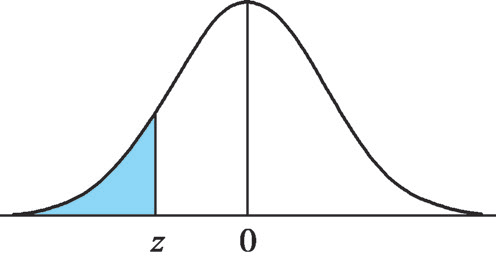
\includegraphics[width=0.25\textwidth]{image/chart1.png} % chart1
    \caption*{附表 1 图示}
\end{figure}

\begin{longtable}{c|cccccccccc}
    \hline
    $z$ & 0.00 & 0.01 & 0.02 & 0.03 & 0.04 & 0.05 & 0.06 & 0.07 & 0.08 & 0.09 \\
    \hline
    \endhead
    $-3.0$ & 0.0013 & 0.0013 & 0.0013 & 0.0012 & 0.0012 & 0.0011 & 0.0011 & 0.0011 & 0.0010 & 0.0010 \\
    $-2.9$ & 0.0019 & 0.0018 & 0.0018 & 0.0017 & 0.0016 & 0.0016 & 0.0015 & 0.0015 & 0.0014 & 0.0014 \\
    $-2.8$ & 0.0026 & 0.0025 & 0.0024 & 0.0023 & 0.0023 & 0.0022 & 0.0021 & 0.0021 & 0.0020 & 0.0019 \\
    $-2.7$ & 0.0035 & 0.0034 & 0.0033 & 0.0032 & 0.0031 & 0.0030 & 0.0029 & 0.0028 & 0.0027 & 0.0026 \\
    $-2.6$ & 0.0047 & 0.0045 & 0.0044 & 0.0043 & 0.0041 & 0.0040 & 0.0039 & 0.0038 & 0.0037 & 0.0036 \\
    $-2.5$ & 0.0062 & 0.0060 & 0.0059 & 0.0057 & 0.0055 & 0.0054 & 0.0052 & 0.0051 & 0.0049 & 0.0048 \\
    $-2.4$ & 0.0082 & 0.0080 & 0.0078 & 0.0075 & 0.0073 & 0.0071 & 0.0069 & 0.0068 & 0.0066 & 0.0064 \\
    $-2.3$ & 0.0107 & 0.0104 & 0.0102 & 0.0099 & 0.0096 & 0.0094 & 0.0091 & 0.0089 & 0.0087 & 0.0084 \\
    $-2.2$ & 0.0139 & 0.0136 & 0.0132 & 0.0129 & 0.0125 & 0.0122 & 0.0119 & 0.0116 & 0.0113 & 0.0110 \\
    $-2.1$ & 0.0179 & 0.0174 & 0.0170 & 0.0166 & 0.0162 & 0.0158 & 0.0154 & 0.0150 & 0.0146 & 0.0143 \\
    $-2.0$ & 0.0228 & 0.0222 & 0.0217 & 0.0212 & 0.0207 & 0.0202 & 0.0197 & 0.0192 & 0.0188 & 0.0183 \\
    $-1.9$ & 0.0287 & 0.0281 & 0.0274 & 0.0268 & 0.0262 & 0.0256 & 0.0250 & 0.0244 & 0.0239 & 0.0233 \\
    $-1.8$ & 0.0359 & 0.0351 & 0.0344 & 0.0336 & 0.0329 & 0.0322 & 0.0314 & 0.0307 & 0.0301 & 0.0294 \\
    $-1.7$ & 0.0446 & 0.0436 & 0.0427 & 0.0418 & 0.0409 & 0.0401 & 0.0392 & 0.0384 & 0.0375 & 0.0367 \\
    $-1.6$ & 0.0548 & 0.0537 & 0.0526 & 0.0516 & 0.0505 & 0.0495 & 0.0485 & 0.0475 & 0.0465 & 0.0455 \\
    $-1.5$ & 0.0668 & 0.0655 & 0.0643 & 0.0630 & 0.0618 & 0.0606 & 0.0594 & 0.0582 & 0.0571 & 0.0559 \\
    $-1.4$ & 0.0808 & 0.0793 & 0.0778 & 0.0764 & 0.0749 & 0.0735 & 0.0721 & 0.0708 & 0.0694 & 0.0681 \\
    $-1.3$ & 0.0968 & 0.0951 & 0.0934 & 0.0918 & 0.0901 & 0.0885 & 0.0869 & 0.0853 & 0.0838 & 0.0823 \\
    $-1.2$ & 0.1151 & 0.1131 & 0.1112 & 0.1093 & 0.1075 & 0.1056 & 0.1038 & 0.1020 & 0.1003 & 0.0985 \\
    $-1.1$ & 0.1357 & 0.1335 & 0.1314 & 0.1292 & 0.1271 & 0.1251 & 0.1230 & 0.1210 & 0.1190 & 0.1170 \\
    $-1.0$ & 0.1587 & 0.1562 & 0.1539 & 0.1515 & 0.1492 & 0.1469 & 0.1446 & 0.1423 & 0.1401 & 0.1379 \\
    $-0.9$ & 0.1841 & 0.1814 & 0.1788 & 0.1762 & 0.1736 & 0.1711 & 0.1685 & 0.1660 & 0.1635 & 0.1611 \\
    $-0.8$ & 0.2119 & 0.2090 & 0.2061 & 0.2033 & 0.2005 & 0.1977 & 0.1949 & 0.1922 & 0.1894 & 0.1867 \\
    $-0.7$ & 0.2420 & 0.2389 & 0.2358 & 0.2327 & 0.2296 & 0.2266 & 0.2236 & 0.2206 & 0.2177 & 0.2148 \\
    $-0.6$ & 0.2743 & 0.2709 & 0.2676 & 0.2643 & 0.2611 & 0.2578 & 0.2546 & 0.2514 & 0.2483 & 0.2451 \\
    $-0.5$ & 0.3085 & 0.3050 & 0.3015 & 0.2981 & 0.2946 & 0.2912 & 0.2877 & 0.2843 & 0.2810 & 0.2776 \\
    $-0.4$ & 0.3446 & 0.3409 & 0.3372 & 0.3336 & 0.3300 & 0.3264 & 0.3228 & 0.3192 & 0.3156 & 0.3121 \\
    $-0.3$ & 0.3821 & 0.3783 & 0.3745 & 0.3707 & 0.3669 & 0.3632 & 0.3594 & 0.3557 & 0.3520 & 0.3483 \\
    $-0.2$ & 0.4207 & 0.4168 & 0.4129 & 0.4090 & 0.4052 & 0.4013 & 0.3974 & 0.3936 & 0.3807 & 0.3859 \\
    $-0.1$ & 0.4602 & 0.4562 & 0.4522 & 0.4483 & 0.4443 & 0.4404 & 0.4364 & 0.4325 & 0.4286 & 0.4247 \\
    $-0.0$ & 0.5000 & 0.4960 & 0.4920 & 0.4880 & 0.4840 & 0.4801 & 0.4761 & 0.4721 & 0.4681 & 0.4641 \\
    \hline
\end{longtable}

\newpage

% ==========================================
% 附表 2 t 分布界值表（双侧尾部面积）
% ==========================================
\section{附表 2 $t$ 分布界值表（双侧尾部面积）}

\begin{figure}[htbp]
    \raggedleft
    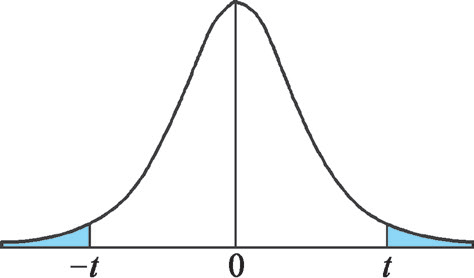
\includegraphics[width=0.25\textwidth]{image/chart2.png} % 请截取原图保存为该文件名
    \caption*{附表 2 图示}
\end{figure}

\begin{longtable}{c|cccccccccc}
    \hline
    自由度 & \multicolumn{10}{c}{概率 $P$} \\
    $v$ & 单侧: 0.25 & 0.20 & 0.10 & 0.05 & 0.025 & 0.01 & 0.005 & 0.0025 & 0.001 & 0.0005 \\
    & 双侧: 0.50 & 0.40 & 0.20 & 0.10 & 0.05 & 0.02 & 0.01 & 0.005 & 0.002 & 0.001 \\
    \hline
    \endhead
    1  & 1.000 & 1.376 & 3.078 & 6.314 & 12.706 & 31.821 & 63.657 & 127.321 & 318.309 & 636.619 \\
    2  & 0.816 & 1.061 & 1.886 & 2.920 & 4.303  & 6.965  & 9.925  & 14.089  & 22.327  & 31.599 \\
    3  & 0.765 & 0.978 & 1.638 & 2.353 & 3.182  & 4.541  & 5.841  & 7.543   & 10.215  & 12.924 \\
    4  & 0.741 & 0.941 & 1.533 & 2.132 & 2.776  & 3.747  & 4.604  & 5.598   & 7.173   & 8.610 \\
    5  & 0.727 & 0.920 & 1.476 & 2.015 & 2.571  & 3.365  & 4.032  & 4.773   & 5.893   & 6.869 \\
    6  & 0.718 & 0.906 & 1.440 & 1.943 & 2.447  & 3.143  & 3.707  & 4.317   & 5.208   & 5.959 \\
    7  & 0.711 & 0.896 & 1.415 & 1.895 & 2.365  & 2.998  & 3.499  & 4.029   & 4.785   & 5.408 \\
    8  & 0.706 & 0.889 & 1.397 & 1.860 & 2.306  & 2.896  & 3.355  & 3.833   & 4.501   & 5.041 \\
    9  & 0.703 & 0.883 & 1.383 & 1.833 & 2.262  & 2.821  & 3.250  & 3.690   & 4.297   & 4.781 \\
    10 & 0.700 & 0.879 & 1.372 & 1.812 & 2.228  & 2.764  & 3.169  & 3.581   & 4.144   & 4.587 \\
    11 & 0.697 & 0.876 & 1.363 & 1.796 & 2.201  & 2.718  & 3.106  & 3.497   & 4.025   & 4.437 \\
    12 & 0.695 & 0.873 & 1.356 & 1.782 & 2.179  & 2.681  & 3.055  & 3.428   & 3.930   & 4.318 \\
    13 & 0.694 & 0.870 & 1.350 & 1.771 & 2.160  & 2.650  & 3.012  & 3.372   & 3.852   & 4.221 \\
    14 & 0.692 & 0.868 & 1.345 & 1.761 & 2.145  & 2.624  & 2.977  & 3.325   & 3.787   & 4.140 \\
    15 & 0.691 & 0.866 & 1.341 & 1.753 & 2.131  & 2.602  & 2.947  & 3.286   & 3.733   & 4.073 \\
    16 & 0.690 & 0.865 & 1.337 & 1.746 & 2.120  & 2.583  & 2.921  & 3.252   & 3.686   & 4.015 \\
    17 & 0.689 & 0.863 & 1.333 & 1.740 & 2.110  & 2.567  & 2.898  & 3.222   & 3.646   & 3.965 \\
    18 & 0.688 & 0.862 & 1.330 & 1.734 & 2.101  & 2.552  & 2.878  & 3.197   & 3.610   & 3.922 \\
    19 & 0.688 & 0.861 & 1.328 & 1.729 & 2.093  & 2.539  & 2.861  & 3.174   & 3.579   & 3.883 \\
    20 & 0.687 & 0.860 & 1.325 & 1.725 & 2.086  & 2.528  & 2.845  & 3.153   & 3.552   & 3.850 \\
    21 & 0.686 & 0.859 & 1.323 & 1.721 & 2.080  & 2.518  & 2.831  & 3.135   & 3.527   & 3.819 \\
    22 & 0.686 & 0.858 & 1.321 & 1.717 & 2.074  & 2.508  & 2.819  & 3.119   & 3.505   & 3.792 \\
    23 & 0.685 & 0.858 & 1.319 & 1.714 & 2.069  & 2.500  & 2.807  & 3.104   & 3.485   & 3.768 \\
    24 & 0.685 & 0.857 & 1.318 & 1.711 & 2.064  & 2.492  & 2.797  & 3.091   & 3.467   & 3.745 \\
    25 & 0.684 & 0.856 & 1.316 & 1.708 & 2.060  & 2.485  & 2.787  & 3.078   & 3.450   & 3.725 \\
    26 & 0.684 & 0.856 & 1.315 & 1.706 & 2.056  & 2.479  & 2.779  & 3.067   & 3.435   & 3.707 \\
    27 & 0.684 & 0.855 & 1.314 & 1.703 & 2.052  & 2.473  & 2.771  & 3.057   & 3.421   & 3.690 \\
    28 & 0.683 & 0.855 & 1.313 & 1.701 & 2.048  & 2.467  & 2.763  & 3.047   & 3.408   & 3.674 \\
    29 & 0.683 & 0.854 & 1.311 & 1.699 & 2.045  & 2.462  & 2.756  & 3.038   & 3.396   & 3.659 \\
    30 & 0.683 & 0.854 & 1.310 & 1.697 & 2.042  & 2.457  & 2.750  & 3.030   & 3.385   & 3.646 \\
    31 & 0.682 & 0.853 & 1.309 & 1.696 & 2.040  & 2.453  & 2.744  & 3.022   & 3.375   & 3.633 \\
    32 & 0.682 & 0.853 & 1.309 & 1.694 & 2.037  & 2.449  & 2.738  & 3.015   & 3.365   & 3.622 \\
    33 & 0.682 & 0.853 & 1.308 & 1.692 & 2.035  & 2.445  & 2.733  & 3.008   & 3.356   & 3.611 \\
    34 & 0.682 & 0.852 & 1.307 & 1.691 & 2.032  & 2.441  & 2.728  & 3.002   & 3.348   & 3.601 \\
    35 & 0.682 & 0.852 & 1.306 & 1.690 & 2.030  & 2.438  & 2.724  & 2.996   & 3.340   & 3.591 \\
    36 & 0.681 & 0.852 & 1.306 & 1.688 & 2.028  & 2.434  & 2.719  & 2.990   & 3.333   & 3.582 \\
    37 & 0.681 & 0.851 & 1.305 & 1.687 & 2.026  & 2.431  & 2.715  & 2.985   & 3.326   & 3.574 \\
    38 & 0.681 & 0.851 & 1.304 & 1.686 & 2.024  & 2.429  & 2.712  & 2.980   & 3.319   & 3.566 \\
    39 & 0.681 & 0.851 & 1.304 & 1.685 & 2.023  & 2.426  & 2.708  & 2.976   & 3.313   & 3.558 \\
    40 & 0.681 & 0.851 & 1.303 & 1.684 & 2.021  & 2.423  & 2.704  & 2.971   & 3.307   & 3.551 \\
    50 & 0.679 & 0.849 & 1.299 & 1.676 & 2.009  & 2.403  & 2.678  & 2.937   & 3.261   & 3.496 \\
    60 & 0.679 & 0.848 & 1.296 & 1.671 & 2.000  & 2.390  & 2.660  & 2.915   & 3.232   & 3.460 \\
    70 & 0.678 & 0.847 & 1.294 & 1.667 & 1.994  & 2.381  & 2.648  & 2.899   & 3.211   & 3.435 \\
    80 & 0.678 & 0.846 & 1.292 & 1.664 & 1.990  & 2.374  & 2.639  & 2.887   & 3.195   & 3.416 \\
    90 & 0.677 & 0.846 & 1.291 & 1.662 & 1.987  & 2.368  & 2.632  & 2.878   & 3.183   & 3.402 \\
    100& 0.677 & 0.845 & 1.290 & 1.660 & 1.984  & 2.364  & 2.626  & 2.871   & 3.174   & 3.390 \\
    200& 0.676 & 0.843 & 1.286 & 1.653 & 1.972  & 2.345  & 2.601  & 2.839   & 3.131   & 3.340 \\
    500& 0.675 & 0.842 & 1.283 & 1.648 & 1.965  & 2.334  & 2.586  & 2.820   & 3.137   & 3.310 \\
    1000&0.675 & 0.842 & 1.282 & 1.646 & 1.962  & 2.330  & 2.581  & 2.813   & 3.098   & 3.300 \\
    $\infty$&0.6745&0.8416&1.2816&1.6449&1.9600& 2.3263 & 2.5758 & 2.8070  & 3.0902  & 3.2905 \\
    \hline
\end{longtable}

\newpage

% ==========================================
% 附表 3 F 分布双侧界值表（P=0.10）
% ==========================================
\section{附表 3 $F$ 分布双侧界值表（方差齐性检验用，$P=0.10$）}

\footnotesize
\begin{longtable}{c|ccccccccccccccc}
    \hline
    $v_2$ & \multicolumn{15}{c}{分子的自由度 $v_1$} \\
    & 1 & 2 & 3 & 4 & 5 & 6 & 7 & 8 & 9 & 10 & 11 & 12 & 15 & 20 & 30 \\
    \hline
    \endhead
    1 & 161.45 & 199.50 & 215.71 & 224.58 & 230.16 & 233.99 & 236.77 & 238.88 & 240.54 & 241.88 & 242.98 & 243.91 & 245.95 & 248.01 & 250.1 \\
    2 & 18.51 & 19.00 & 19.16 & 19.25 & 19.30 & 19.33 & 19.35 & 19.37 & 19.38 & 19.4 & 19.40 & 19.41 & 19.43 & 19.45 & 19.46 \\
    3 & 10.13 & 9.55 & 9.28 & 9.12 & 9.01 & 8.94 & 8.89 & 8.85 & 8.81 & 8.79 & 8.76 & 8.74 & 8.70 & 8.66 & 8.62 \\
    4 & 7.71 & 6.94 & 6.59 & 6.39 & 6.26 & 6.16 & 6.09 & 6.04 & 6.00 & 5.96 & 5.94 & 5.91 & 5.86 & 5.80 & 5.75 \\
    5 & 6.61 & 5.79 & 5.41 & 5.19 & 5.05 & 4.95 & 4.88 & 4.82 & 4.77 & 4.74 & 4.70 & 4.68 & 4.62 & 4.56 & 4.50 \\
    6 & 5.99 & 5.14 & 4.76 & 4.53 & 4.39 & 4.28 & 4.21 & 4.15 & 4.10 & 4.06 & 4.03 & 4.00 & 3.94 & 3.87 & 3.81 \\
    7 & 5.59 & 4.74 & 4.35 & 4.12 & 3.97 & 3.87 & 3.79 & 3.73 & 3.68 & 3.64 & 3.60 & 3.57 & 3.51 & 3.44 & 3.38 \\
    8 & 5.32 & 4.46 & 4.07 & 3.84 & 3.69 & 3.58 & 3.50 & 3.44 & 3.39 & 3.35 & 3.31 & 3.28 & 3.22 & 3.15 & 3.08 \\
    9 & 5.12 & 4.26 & 3.86 & 3.63 & 3.48 & 3.37 & 3.29 & 3.23 & 3.18 & 3.14 & 3.10 & 3.07 & 3.01 & 2.94 & 2.86 \\
    10 & 4.96 & 4.10 & 3.71 & 3.48 & 3.33 & 3.22 & 3.14 & 3.07 & 3.02 & 2.98 & 2.94 & 2.91 & 2.85 & 2.77 & 2.70 \\
    11 & 4.84 & 3.98 & 3.59 & 3.36 & 3.20 & 3.09 & 3.01 & 2.95 & 2.90 & 2.85 & 2.82 & 2.79 & 2.72 & 2.65 & 2.57 \\
    12 & 4.75 & 3.89 & 3.49 & 3.26 & 3.11 & 3.00 & 2.91 & 2.85 & 2.80 & 2.75 & 2.72 & 2.69 & 2.62 & 2.54 & 2.47 \\
    13 & 4.67 & 3.81 & 3.41 & 3.18 & 3.03 & 2.92 & 2.83 & 2.77 & 2.71 & 2.67 & 2.63 & 2.60 & 2.53 & 2.46 & 2.38 \\
    14 & 4.60 & 3.74 & 3.34 & 3.11 & 2.96 & 2.85 & 2.76 & 2.70 & 2.65 & 2.60 & 2.57 & 2.53 & 2.46 & 2.39 & 2.31 \\
    15 & 4.54 & 3.68 & 3.29 & 3.06 & 2.90 & 2.79 & 2.71 & 2.64 & 2.59 & 2.54 & 2.51 & 2.48 & 2.40 & 2.33 & 2.25 \\
    16 & 4.49 & 3.63 & 3.24 & 3.01 & 2.85 & 2.74 & 2.66 & 2.59 & 2.54 & 2.49 & 2.46 & 2.42 & 2.35 & 2.28 & 2.19 \\
    17 & 4.45 & 3.59 & 3.20 & 2.96 & 2.81 & 2.70 & 2.61 & 2.55 & 2.49 & 2.45 & 2.41 & 2.38 & 2.31 & 2.23 & 2.15 \\
    18 & 4.41 & 3.55 & 3.16 & 2.93 & 2.77 & 2.66 & 2.58 & 2.51 & 2.46 & 2.41 & 2.37 & 2.34 & 2.27 & 2.19 & 2.11 \\
    19 & 4.38 & 3.52 & 3.13 & 2.90 & 2.74 & 2.63 & 2.54 & 2.48 & 2.42 & 2.38 & 2.34 & 2.31 & 2.23 & 2.16 & 2.07 \\
    20 & 4.35 & 3.49 & 3.10 & 2.87 & 2.71 & 2.60 & 2.51 & 2.45 & 2.39 & 2.35 & 2.31 & 2.28 & 2.20 & 2.12 & 2.04 \\
    21 & 4.32 & 3.47 & 3.07 & 2.84 & 2.68 & 2.57 & 2.49 & 2.42 & 2.37 & 2.32 & 2.28 & 2.25 & 2.18 & 2.10 & 2.01 \\
    22 & 4.30 & 3.44 & 3.05 & 2.82 & 2.66 & 2.55 & 2.46 & 2.40 & 2.34 & 2.30 & 2.26 & 2.23 & 2.15 & 2.07 & 1.98 \\
    23 & 4.28 & 3.42 & 3.03 & 2.80 & 2.64 & 2.53 & 2.44 & 2.37 & 2.32 & 2.27 & 2.24 & 2.20 & 2.13 & 2.05 & 1.96 \\
    24 & 4.26 & 3.40 & 3.01 & 2.78 & 2.62 & 2.51 & 2.42 & 2.36 & 2.30 & 2.25 & 2.22 & 2.18 & 2.11 & 2.03 & 1.94 \\
    25 & 4.24 & 3.39 & 2.99 & 2.76 & 2.60 & 2.49 & 2.40 & 2.34 & 2.28 & 2.24 & 2.20 & 2.16 & 2.09 & 2.01 & 1.92 \\
    26 & 4.23 & 3.37 & 2.98 & 2.74 & 2.59 & 2.47 & 2.39 & 2.32 & 2.27 & 2.22 & 2.18 & 2.15 & 2.07 & 1.99 & 1.90 \\
    27 & 4.21 & 3.35 & 2.96 & 2.73 & 2.57 & 2.46 & 2.37 & 2.31 & 2.25 & 2.20 & 2.17 & 2.13 & 2.06 & 1.97 & 1.88 \\
    28 & 4.20 & 3.34 & 2.95 & 2.71 & 2.56 & 2.45 & 2.36 & 2.29 & 2.24 & 2.19 & 2.15 & 2.12 & 2.04 & 1.96 & 1.87 \\
    29 & 4.18 & 3.33 & 2.93 & 2.70 & 2.55 & 2.43 & 2.35 & 2.28 & 2.22 & 2.18 & 2.14 & 2.10 & 2.03 & 1.94 & 1.85 \\
    30 & 4.17 & 3.32 & 2.92 & 2.69 & 2.53 & 2.42 & 2.33 & 2.27 & 2.21 & 2.16 & 2.13 & 2.09 & 2.01 & 1.93 & 1.84 \\
    40 & 4.08 & 3.23 & 2.84 & 2.61 & 2.45 & 2.34 & 2.25 & 2.18 & 2.12 & 2.08 & 2.04 & 2.00 & 1.92 & 1.84 & 1.74 \\
    60 & 4.00 & 3.15 & 2.76 & 2.53 & 2.37 & 2.25 & 2.17 & 2.10 & 2.04 & 1.99 & 1.95 & 1.92 & 1.84 & 1.75 & 1.65 \\
    120 & 3.92 & 3.07 & 2.68 & 2.45 & 2.29 & 2.18 & 2.09 & 2.02 & 1.96 & 1.91 & 1.87 & 1.83 & 1.75 & 1.66 & 1.55 \\
    $\infty$ & 3.84 & 3.00 & 2.60 & 2.37 & 2.21 & 2.10 & 2.01 & 1.94 & 1.88 & 1.83 & 1.79 & 1.75 & 1.67 & 1.57 & 1.46 \\
    \hline
\end{longtable}
\normalsize

\newpage

% ==========================================
% 附表 4 F 界值表（单侧）
% ==========================================
\section{附表 4 $F$ 界值表（方差分析用，单侧界值）}
\noindent
\textbf{说明}：表中上行数据为 $P=0.05$ 界值，下行数据为 $P=0.01$ 界值。

\begin{figure}[htbp]
    \raggedleft
    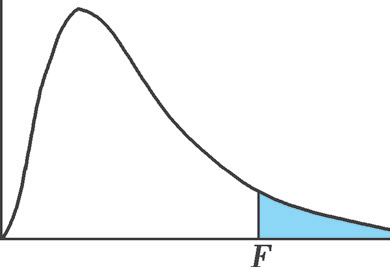
\includegraphics[width=0.25\textwidth]{image/chart4.png}
    \caption*{附表 4 图示}
\end{figure}

\subsection{第一部分：$v_1 = 1 \sim 12$}
\footnotesize
\begin{longtable}{c|ccccccccccc}
    \hline
    $v_2$ & \multicolumn{11}{c}{$v_1$} \\
    & 1 & 2 & 3 & 4 & 5 & 6 & 7 & 8 & 9 & 10 & 11 \dots \\
    \hline
    \endhead
    1 & 161 & 200 & 216 & 225 & 230 & 234 & 237 & 239 & 241 & 242 & 243 \\
      & 4052 & 4999 & 5403 & 5625 & 5764 & 5859 & 5928 & 5981 & 6022 & 6056 & 6082 \\
    2 & 18.51 & 19.00 & 19.16 & 19.25 & 19.30 & 19.33 & 19.36 & 19.37 & 19.38 & 19.39 & 19.40 \\
      & 98.49 & 99.00 & 99.17 & 99.25 & 99.30 & 99.33 & 99.34 & 99.36 & 99.38 & 99.40 & 99.41 \\
    3 & 10.13 & 9.55 & 9.28 & 9.12 & 9.01 & 8.94 & 8.88 & 8.84 & 8.81 & 8.78 & 8.76 \\
      & 34.12 & 30.82 & 29.46 & 28.71 & 28.24 & 27.91 & 27.67 & 27.49 & 27.34 & 27.23 & 27.31 \\
    4 & 7.71 & 6.94 & 6.59 & 6.39 & 6.26 & 6.16 & 6.09 & 6.04 & 6.00 & 5.96 & 5.93 \\
      & 21.20 & 18.00 & 16.59 & 15.98 & 15.52 & 15.21 & 14.98 & 14.80 & 14.66 & 14.54 & 14.45 \\
    5 & 6.61 & 5.79 & 5.41 & 5.19 & 5.05 & 4.95 & 4.88 & 4.82 & 4.78 & 4.74 & 4.70 \\
      & 16.26 & 13.27 & 12.06 & 11.39 & 10.97 & 10.67 & 10.45 & 10.27 & 10.15 & 10.05 & 9.96 \\
    6 & 5.99 & 5.15 & 4.76 & 4.53 & 4.39 & 4.28 & 4.21 & 4.15 & 4.10 & 4.06 & 4.03 \\
      & 13.74 & 10.92 & 9.78 & 9.15 & 8.75 & 8.47 & 8.26 & 8.10 & 7.98 & 7.87 & 7.79 \\
    7 & 5.59 & 4.74 & 4.35 & 4.12 & 3.97 & 3.87 & 3.79 & 3.73 & 3.68 & 3.63 & 3.60 \\
      & 12.25 & 9.55 & 8.45 & 7.85 & 7.46 & 7.19 & 7.00 & 6.84 & 6.71 & 6.62 & 6.54 \\
    8 & 5.32 & 4.46 & 4.07 & 3.84 & 3.69 & 3.58 & 3.50 & 3.44 & 3.39 & 3.34 & 3.31 \\
      & 11.26 & 8.65 & 7.59 & 7.01 & 6.63 & 6.37 & 6.19 & 6.03 & 5.91 & 5.82 & 5.74 \\
    9 & 5.12 & 4.26 & 3.86 & 3.63 & 3.48 & 3.37 & 3.29 & 3.23 & 3.18 & 3.13 & 3.10 \\
      & 10.56 & 8.02 & 6.99 & 6.42 & 6.06 & 5.80 & 5.62 & 5.47 & 5.35 & 5.26 & 5.18 \\
    10 & 4.69 & 4.10 & 3.71 & 3.48 & 3.33 & 3.22 & 3.14 & 3.07 & 3.02 & 2.97 & 2.94 \\
      & 10.04 & 7.56 & 6.55 & 5.09 & 5.64 & 5.39 & 5.21 & 5.06 & 4.95 & 4.85 & 4.78 \\
    11 & 4.84 & 3.98 & 3.59 & 3.36 & 3.20 & 3.09 & 3.01 & 2.95 & 2.90 & 2.86 & 2.82 \\
       & 9.65 & 7.20 & 6.22 & 5.67 & 5.32 & 5.07 & 4.88 & 4.74 & 4.63 & 4.54 & 4.46 \\
    12 & 4.75 & 3.88 & 3.49 & 3.26 & 3.11 & 3.00 & 2.92 & 2.85 & 2.80 & 2.76 & 2.72 \\
       & 9.33 & 6.93 & 5.95 & 5.41 & 5.06 & 4.82 & 4.65 & 4.50 & 4.39 & 4.30 & 4.22 \\
    13 & 4.67 & 3.80 & 3.41 & 3.18 & 3.02 & 2.92 & 2.84 & 2.77 & 2.72 & 2.67 & 2.63 \\
       & 9.07 & 6.70 & 5.74 & 5.20 & 4.85 & 4.62 & 4.44 & 4.30 & 4.19 & 4.10 & 4.02 \\
    14 & 4.60 & 3.74 & 3.34 & 3.11 & 2.96 & 2.85 & 2.77 & 2.70 & 2.65 & 2.60 & 2.56 \\
       & 8.86 & 6.51 & 5.56 & 5.03 & 4.69 & 4.46 & 4.28 & 4.14 & 4.03 & 3.94 & 3.86 \\
    15 & 4.54 & 3.68 & 3.29 & 3.06 & 2.90 & 2.79 & 2.70 & 2.64 & 2.59 & 2.55 & 2.51 \\
       & 8.68 & 6.36 & 5.42 & 4.89 & 4.56 & 4.32 & 4.14 & 4.00 & 3.89 & 3.80 & 3.73 \\
    16 & 4.49 & 3.63 & 3.24 & 3.01 & 2.85 & 2.74 & 2.66 & 2.59 & 2.54 & 2.49 & 2.45 \\
       & 8.53 & 6.23 & 5.29 & 4.77 & 4.44 & 4.20 & 4.03 & 3.89 & 3.78 & 3.69 & 3.61 \\
    17 & 4.45 & 3.59 & 3.20 & 2.96 & 2.81 & 2.70 & 2.62 & 2.55 & 2.50 & 2.45 & 2.41 \\
       & 8.40 & 6.11 & 5.18 & 4.67 & 4.34 & 4.10 & 3.93 & 3.79 & 3.68 & 3.59 & 3.52 \\
    18 & 4.41 & 3.55 & 3.16 & 2.93 & 2.77 & 2.66 & 2.58 & 2.51 & 2.46 & 2.41 & 2.37 \\
       & 8.28 & 6.01 & 5.09 & 4.58 & 4.25 & 4.01 & 3.85 & 3.71 & 3.60 & 3.51 & 3.44 \\
    19 & 4.38 & 3.52 & 3.13 & 2.90 & 2.74 & 2.63 & 2.55 & 2.48 & 2.43 & 2.38 & 2.34 \\
       & 8.18 & 5.93 & 5.01 & 4.50 & 4.17 & 3.94 & 3.77 & 3.63 & 3.52 & 3.43 & 3.36 \\
    20 & 4.35 & 3.49 & 3.10 & 2.87 & 2.71 & 2.60 & 2.52 & 2.45 & 2.40 & 2.35 & 2.31 \\
       & 8.10 & 5.85 & 4.94 & 4.43 & 4.10 & 3.87 & 3.71 & 3.56 & 3.45 & 3.37 & 3.30 \\
    21 & 4.32 & 3.47 & 3.07 & 2.84 & 2.68 & 2.57 & 2.49 & 2.42 & 2.37 & 2.32 & 2.28 \\
       & 8.02 & 5.78 & 4.87 & 4.37 & 4.04 & 3.81 & 3.65 & 3.51 & 3.40 & 3.31 & 3.24 \\
    22 & 4.30 & 3.44 & 3.05 & 2.82 & 2.66 & 2.55 & 2.47 & 2.40 & 2.35 & 2.30 & 2.26 \\
       & 7.94 & 5.72 & 4.82 & 4.31 & 3.99 & 3.76 & 3.59 & 3.45 & 3.35 & 3.26 & 3.18 \\
    23 & 4.28 & 3.42 & 3.03 & 2.80 & 2.64 & 2.53 & 2.45 & 2.38 & 2.32 & 2.28 & 2.24 \\
       & 7.88 & 5.66 & 4.76 & 4.86 & 3.94 & 3.71 & 3.54 & 3.41 & 3.30 & 3.21 & 3.14 \\
    24 & 4.26 & 3.40 & 3.01 & 2.78 & 2.62 & 2.51 & 2.43 & 2.36 & 2.30 & 2.26 & 2.22 \\
       & 7.82 & 5.61 & 4.72 & 4.22 & 3.90 & 3.67 & 3.50 & 3.36 & 3.25 & 3.17 & 3.09 \\
    25 & 4.24 & 3.38 & 2.99 & 2.76 & 2.60 & 2.49 & 2.41 & 2.34 & 2.28 & 2.24 & 2.20 \\
       & 7.77 & 5.57 & 4.68 & 4.18 & 3.86 & 3.63 & 3.46 & 3.32 & 3.21 & 3.13 & 3.05 \\
    26 & 4.22 & 3.37 & 2.98 & 2.74 & 2.59 & 2.47 & 2.39 & 2.32 & 2.27 & 2.22 & 2.18 \\
       & 7.72 & 5.53 & 4.64 & 4.14 & 3.82 & 3.59 & 3.42 & 3.29 & 3.17 & 3.09 & 3.02 \\
    27 & 4.21 & 3.35 & 2.96 & 2.73 & 2.57 & 2.46 & 2.37 & 2.30 & 2.25 & 2.20 & 2.16 \\
       & 7.68 & 5.49 & 4.60 & 4.11 & 3.79 & 3.56 & 3.39 & 3.26 & 3.14 & 3.06 & 2.98 \\
    28 & 4.20 & 3.34 & 2.95 & 2.71 & 2.56 & 2.44 & 2.36 & 2.29 & 2.24 & 2.19 & 2.15 \\
       & 7.64 & 5.45 & 4.57 & 4.07 & 3.76 & 3.53 & 3.36 & 3.23 & 3.11 & 3.03 & 2.95 \\
    29 & 4.18 & 3.33 & 2.93 & 2.70 & 2.54 & 2.43 & 2.35 & 2.28 & 2.22 & 2.18 & 2.14 \\
       & 7.60 & 5.42 & 4.54 & 4.04 & 3.73 & 3.50 & 3.33 & 3.20 & 3.08 & 3.00 & 2.92 \\
    30 & 4.17 & 3.32 & 2.92 & 2.69 & 2.53 & 2.42 & 2.34 & 2.27 & 2.21 & 2.16 & 2.12 \\
       & 7.56 & 5.39 & 4.51 & 4.02 & 3.70 & 3.47 & 3.30 & 3.17 & 3.06 & 2.98 & 2.91 \\
    32 & 4.15 & 3.30 & 2.90 & 2.67 & 2.51 & 2.40 & 2.32 & 2.25 & 2.19 & 2.14 & 2.10 \\
       & 7.50 & 5.35 & 4.46 & 3.97 & 3.66 & 3.42 & 3.25 & 3.12 & 3.01 & 2.94 & 2.86 \\
    34 & 4.13 & 3.28 & 2.88 & 2.65 & 2.49 & 2.38 & 2.30 & 2.23 & 2.17 & 2.12 & 2.08 \\
       & 7.44 & 5.29 & 4.42 & 3.93 & 3.61 & 3.38 & 3.21 & 3.08 & 2.98 & 2.89 & 2.82 \\
    36 & 4.11 & 3.26 & 2.86 & 2.63 & 2.48 & 2.36 & 2.28 & 2.21 & 2.15 & 2.10 & 2.06 \\
       & 7.39 & 5.25 & 4.38 & 3.89 & 3.58 & 3.35 & 3.18 & 3.04 & 2.94 & 2.86 & 2.78 \\
    38 & 4.10 & 3.25 & 2.85 & 2.62 & 2.46 & 2.35 & 2.26 & 2.19 & 2.14 & 2.09 & 2.05 \\
       & 7.35 & 5.21 & 4.31 & 3.86 & 3.54 & 3.32 & 3.15 & 3.02 & 2.91 & 2.82 & 2.75 \\
    40 & 4.08 & 3.23 & 2.84 & 2.61 & 2.45 & 2.34 & 2.25 & 2.18 & 2.12 & 2.07 & 2.04 \\
       & 7.31 & 5.18 & 4.31 & 3.83 & 3.51 & 3.29 & 3.12 & 2.99 & 2.88 & 2.80 & 2.73 \\
    42 & 4.07 & 3.22 & 2.83 & 2.59 & 2.44 & 2.32 & 2.24 & 2.17 & 2.11 & 2.06 & 2.02 \\
       & 7.27 & 5.15 & 4.29 & 3.80 & 3.49 & 3.26 & 3.10 & 2.96 & 2.86 & 2.77 & 2.70 \\
    44 & 4.06 & 3.21 & 2.82 & 2.58 & 2.43 & 2.31 & 2.23 & 2.16 & 2.10 & 2.05 & 2.01 \\
       & 7.24 & 5.12 & 4.26 & 3.78 & 3.46 & 3.24 & 3.07 & 2.94 & 2.84 & 2.75 & 2.68 \\
    46 & 4.05 & 3.20 & 2.81 & 2.57 & 2.42 & 2.30 & 2.22 & 2.14 & 2.09 & 2.04 & 2.00 \\
       & 7.21 & 5.10 & 4.24 & 3.76 & 3.44 & 3.22 & 3.05 & 2.92 & 2.82 & 2.73 & 2.66 \\
    48 & 4.04 & 3.19 & 2.80 & 2.56 & 2.41 & 2.30 & 2.21 & 2.14 & 2.08 & 2.03 & 1.99 \\
       & 7.19 & 5.08 & 4.22 & 3.74 & 3.42 & 3.20 & 3.04 & 2.90 & 2.80 & 2.71 & 2.64 \\
    50 & 4.03 & 3.18 & 2.79 & 2.56 & 2.40 & 2.29 & 2.20 & 2.13 & 2.07 & 2.02 & 1.98 \\
       & 7.17 & 5.06 & 4.20 & 3.72 & 3.41 & 3.18 & 3.02 & 2.88 & 2.78 & 2.70 & 2.62 \\
    60 & 4.00 & 3.15 & 2.76 & 2.52 & 2.37 & 2.25 & 2.17 & 2.10 & 2.04 & 1.99 & 1.95 \\
       & 7.08 & 4.98 & 4.13 & 3.65 & 3.34 & 3.12 & 2.95 & 2.82 & 2.72 & 2.63 & 2.56 \\
    70 & 3.98 & 3.13 & 2.74 & 2.50 & 2.35 & 2.23 & 2.14 & 2.07 & 2.01 & 1.97 & 1.93 \\
       & 7.01 & 4.92 & 4.08 & 3.60 & 3.29 & 3.07 & 2.91 & 2.77 & 2.67 & 2.59 & 2.51 \\
    80 & 3.96 & 3.11 & 2.72 & 2.48 & 2.33 & 2.21 & 2.12 & 2.05 & 1.99 & 1.95 & 1.91 \\
       & 6.96 & 4.88 & 4.04 & 3.56 & 3.25 & 3.04 & 2.87 & 2.74 & 2.64 & 2.55 & 2.48 \\
    100& 3.94 & 3.09 & 2.70 & 2.46 & 2.30 & 2.19 & 2.10 & 2.03 & 1.97 & 1.92 & 1.88 \\
       & 6.90 & 4.82 & 3.98 & 3.51 & 3.20 & 2.99 & 2.82 & 2.69 & 2.59 & 2.51 & 2.43 \\
    125& 3.92 & 3.07 & 2.68 & 2.44 & 2.29 & 2.17 & 2.08 & 2.01 & 1.95 & 1.90 & 1.86 \\
       & 6.84 & 4.78 & 3.94 & 3.47 & 3.17 & 2.95 & 2.79 & 2.65 & 2.56 & 2.47 & 2.40 \\
    150& 3.91 & 3.06 & 2.67 & 2.43 & 2.27 & 2.16 & 2.07 & 2.00 & 1.94 & 1.89 & 1.85 \\
       & 6.81 & 4.75 & 3.91 & 3.44 & 3.14 & 2.92 & 2.76 & 2.62 & 2.53 & 2.44 & 2.37 \\
    200& 3.89 & 3.04 & 2.65 & 2.41 & 2.26 & 2.14 & 2.05 & 1.98 & 1.92 & 1.87 & 1.83 \\
       & 6.76 & 4.71 & 3.88 & 3.41 & 3.11 & 2.90 & 2.73 & 2.60 & 2.50 & 2.41 & 2.34 \\
    400& 3.86 & 3.02 & 2.62 & 2.39 & 2.23 & 2.12 & 2.03 & 1.96 & 1.90 & 1.85 & 1.81 \\
       & 6.70 & 4.66 & 3.83 & 3.36 & 3.06 & 2.85 & 2.69 & 2.55 & 2.46 & 2.37 & 2.29 \\
    1000&3.85 & 3.00 & 2.61 & 2.38 & 2.22 & 2.10 & 2.02 & 1.95 & 1.89 & 1.84 & 1.80 \\
       & 6.66 & 4.62 & 3.80 & 3.34 & 3.04 & 2.82 & 2.66 & 2.53 & 2.43 & 2.34 & 2.26 \\
    $\infty$&3.84&2.99&2.60&2.37&2.21&2.09&2.01&1.94&1.88&1.83&1.79 \\
       & 6.64 & 4.60 & 3.78 & 3.32 & 3.02 & 2.80 & 2.64 & 2.51 & 2.41 & 2.32 & 2.24 \\
    \hline
\end{longtable}

\subsection{第二部分：$v_1 = 14 \sim \infty$}
\begin{longtable}{c|ccccccccc}
    \hline
    $v_2$ & \multicolumn{9}{c}{$v_1$} \\
    & 14 & 16 & 20 & 24 & 30 & 40 & 50 & 75 & 100 \dots \\
    \hline
    \endhead
    1 & 245 & 246 & 248 & 249 & 250 & 251 & 252 & 253 & 253 \\
      & 6142 & 6169 & 6208 & 6234 & 6258 & 6286 & 6302 & 6323 & 6334 \\
    2 & 19.42 & 19.43 & 19.44 & 19.45 & 19.46 & 19.47 & 19.47 & 19.48 & 19.49 \\
      & 99.43 & 99.44 & 99.45 & 99.46 & 99.47 & 99.48 & 99.48 & 99.49 & 99.49 \\
    3 & 8.71 & 8.69 & 8.66 & 8.64 & 8.62 & 8.60 & 8.58 & 8.57 & 8.56 \\
      & 26.92 & 26.83 & 26.69 & 26.60 & 26.50 & 26.41 & 26.35 & 26.27 & 26.23 \\
    4 & 5.87 & 5.84 & 5.80 & 5.77 & 5.74 & 5.71 & 5.70 & 5.68 & 5.66 \\
      & 14.24 & 14.15 & 14.02 & 13.93 & 13.83 & 13.74 & 13.69 & 13.61 & 13.57 \\
    5 & 4.64 & 4.60 & 4.56 & 4.53 & 4.50 & 4.46 & 4.44 & 4.42 & 4.40 \\
      & 9.77 & 9.68 & 9.55 & 9.47 & 9.38 & 9.29 & 9.24 & 9.17 & 9.13 \\
    6 & 3.96 & 3.92 & 3.87 & 3.84 & 3.81 & 3.77 & 3.75 & 3.72 & 3.71 \\
      & 7.60 & 7.52 & 7.39 & 7.31 & 7.23 & 7.14 & 7.09 & 7.02 & 6.99 \\
    7 & 3.52 & 3.49 & 3.44 & 3.41 & 3.38 & 3.34 & 3.32 & 3.29 & 3.28 \\
      & 6.35 & 6.27 & 6.15 & 6.07 & 5.98 & 5.90 & 5.85 & 5.78 & 5.75 \\
    8 & 3.23 & 3.20 & 3.15 & 3.12 & 3.08 & 3.05 & 3.03 & 3.00 & 2.98 \\
      & 5.56 & 5.48 & 5.36 & 5.28 & 5.20 & 5.11 & 5.06 & 5.00 & 4.96 \\
    9 & 3.02 & 2.98 & 2.93 & 2.90 & 2.86 & 2.82 & 2.80 & 2.77 & 2.76 \\
      & 5.00 & 4.92 & 4.80 & 4.73 & 4.64 & 4.56 & 4.51 & 4.45 & 4.41 \\
    10& 2.86 & 2.82 & 2.77 & 2.74 & 2.70 & 2.67 & 2.64 & 2.61 & 2.59 \\
      & 4.60 & 4.52 & 4.41 & 4.33 & 4.25 & 4.17 & 4.12 & 4.05 & 4.01 \\
    11& 2.74 & 2.70 & 2.65 & 2.61 & 2.57 & 2.53 & 2.50 & 2.47 & 2.45 \\
      & 4.29 & 4.21 & 4.10 & 4.02 & 3.94 & 3.86 & 3.80 & 3.74 & 3.70 \\
    12& 2.64 & 2.60 & 2.54 & 2.50 & 2.46 & 2.42 & 2.40 & 2.36 & 2.35 \\
      & 4.05 & 3.98 & 3.86 & 3.78 & 3.70 & 3.61 & 3.56 & 3.49 & 3.46 \\
    13& 2.55 & 2.51 & 2.46 & 2.42 & 2.38 & 2.34 & 2.32 & 2.28 & 2.26 \\
      & 3.85 & 3.78 & 3.67 & 3.59 & 3.51 & 3.42 & 3.37 & 3.30 & 3.27 \\
    14& 2.48 & 2.44 & 2.39 & 2.35 & 2.31 & 2.27 & 2.24 & 2.21 & 2.19 \\
      & 3.70 & 3.52 & 3.51 & 3.43 & 3.34 & 3.26 & 3.21 & 3.14 & 3.11 \\
    15& 2.43 & 2.39 & 2.33 & 2.29 & 2.25 & 2.21 & 2.18 & 2.15 & 2.12 \\
      & 3.56 & 3.48 & 3.36 & 3.29 & 3.20 & 3.12 & 3.07 & 3.00 & 2.97 \\
    16& 2.37 & 2.33 & 2.28 & 2.24 & 2.20 & 2.16 & 2.13 & 2.09 & 2.07 \\
      & 3.45 & 3.37 & 3.25 & 3.18 & 3.10 & 3.01 & 2.96 & 2.89 & 2.86 \\
    17& 2.33 & 2.29 & 2.23 & 2.19 & 2.15 & 2.11 & 2.08 & 2.04 & 2.02 \\
      & 3.35 & 3.27 & 3.16 & 3.08 & 3.00 & 2.92 & 2.86 & 2.79 & 2.76 \\
    18& 2.29 & 2.25 & 2.19 & 2.15 & 2.11 & 2.07 & 2.04 & 2.00 & 1.98 \\
      & 3.27 & 3.19 & 3.07 & 3.00 & 2.91 & 2.83 & 2.78 & 2.71 & 2.68 \\
    19& 2.26 & 2.21 & 2.15 & 2.11 & 2.07 & 2.02 & 2.00 & 1.96 & 1.94 \\
      & 3.19 & 3.12 & 3.00 & 2.92 & 2.84 & 2.76 & 2.70 & 2.63 & 2.60 \\
    20& 2.23 & 2.18 & 2.12 & 2.08 & 2.04 & 1.99 & 1.96 & 1.92 & 1.90 \\
      & 3.13 & 3.05 & 2.94 & 2.86 & 2.77 & 2.69 & 2.63 & 2.56 & 2.53 \\
    21& 2.20 & 2.15 & 2.09 & 2.05 & 2.00 & 1.96 & 1.93 & 1.89 & 1.87 \\
      & 3.07 & 2.99 & 2.88 & 2.80 & 2.72 & 2.63 & 2.58 & 2.51 & 2.47 \\
    22& 2.18 & 2.13 & 2.07 & 2.03 & 1.98 & 1.93 & 1.91 & 1.87 & 1.84 \\
      & 3.02 & 2.94 & 2.83 & 2.75 & 2.67 & 2.58 & 2.53 & 2.46 & 2.42 \\
    23& 2.14 & 2.10 & 2.04 & 2.00 & 1.96 & 1.91 & 1.88 & 1.84 & 1.82 \\
      & 2.97 & 2.89 & 2.78 & 2.70 & 2.62 & 2.53 & 2.48 & 2.41 & 2.37 \\
    24& 2.13 & 2.09 & 2.02 & 1.98 & 1.94 & 1.89 & 1.86 & 1.82 & 1.80 \\
      & 2.93 & 2.85 & 2.74 & 2.66 & 2.58 & 2.49 & 2.44 & 2.36 & 2.33 \\
    25& 2.11 & 2.06 & 2.00 & 1.96 & 1.92 & 1.87 & 1.84 & 1.80 & 1.77 \\
      & 2.89 & 2.81 & 2.70 & 2.62 & 2.54 & 2.45 & 2.40 & 2.32 & 2.29 \\
    26& 2.10 & 2.05 & 1.99 & 1.95 & 1.90 & 1.85 & 1.82 & 1.78 & 1.76 \\
      & 2.86 & 2.77 & 2.66 & 2.58 & 2.50 & 2.41 & 2.36 & 2.28 & 2.25 \\
    27& 2.08 & 2.03 & 1.97 & 1.93 & 1.88 & 1.84 & 1.80 & 1.76 & 1.74 \\
      & 2.83 & 2.74 & 2.63 & 2.55 & 2.47 & 2.38 & 2.33 & 2.25 & 2.21 \\
    28& 2.06 & 2.02 & 1.96 & 1.91 & 1.87 & 1.81 & 1.78 & 1.75 & 1.72 \\
      & 2.80 & 2.71 & 2.60 & 2.52 & 2.44 & 2.35 & 2.30 & 2.22 & 2.18 \\
    29& 2.05 & 2.00 & 1.94 & 1.90 & 1.85 & 1.80 & 1.77 & 1.73 & 1.71 \\
      & 2.77 & 2.68 & 2.57 & 2.49 & 2.41 & 2.32 & 2.27 & 2.19 & 2.15 \\
    30& 2.04 & 1.99 & 1.93 & 1.89 & 1.84 & 1.79 & 1.76 & 1.72 & 1.69 \\
      & 2.74 & 2.66 & 2.55 & 2.47 & 2.38 & 2.29 & 2.24 & 2.16 & 2.13 \\
    32& 2.02 & 1.97 & 1.91 & 1.86 & 1.82 & 1.76 & 1.74 & 1.69 & 1.67 \\
      & 2.70 & 2.62 & 2.51 & 2.42 & 2.34 & 2.25 & 2.20 & 2.12 & 2.08 \\
    34& 2.00 & 1.95 & 1.89 & 1.84 & 1.80 & 1.74 & 1.71 & 1.67 & 1.64 \\
      & 2.66 & 2.58 & 2.47 & 2.38 & 2.30 & 2.21 & 2.15 & 2.08 & 2.04 \\
    36& 1.98 & 1.93 & 1.87 & 1.82 & 1.78 & 1.83 & 1.69 & 1.65 & 1.62 \\
      & 2.62 & 2.54 & 2.43 & 2.35 & 2.26 & 2.17 & 2.12 & 2.04 & 2.00 \\
    38& 1.96 & 1.92 & 1.85 & 1.80 & 1.76 & 1.71 & 1.67 & 1.63 & 1.60 \\
      & 2.59 & 2.51 & 2.40 & 2.32 & 2.22 & 2.14 & 2.08 & 2.00 & 1.97 \\
    40& 1.95 & 1.90 & 1.84 & 1.79 & 1.74 & 1.69 & 1.66 & 1.61 & 1.59 \\
      & 2.56 & 2.49 & 2.37 & 2.29 & 2.20 & 2.11 & 2.05 & 1.97 & 1.94 \\
    42& 1.94 & 1.89 & 1.82 & 1.78 & 1.73 & 1.68 & 1.64 & 1.60 & 1.57 \\
      & 2.54 & 2.46 & 2.35 & 2.26 & 2.17 & 2.08 & 2.02 & 1.94 & 1.91 \\
    44& 1.92 & 1.88 & 1.81 & 1.76 & 1.72 & 1.66 & 1.63 & 1.58 & 1.56 \\
      & 2.52 & 2.44 & 2.32 & 2.24 & 2.15 & 2.06 & 2.00 & 1.92 & 1.88 \\
    46& 1.91 & 1.87 & 1.80 & 1.75 & 1.71 & 1.65 & 1.62 & 1.57 & 1.54 \\
      & 2.50 & 2.42 & 2.30 & 2.22 & 2.13 & 2.04 & 1.98 & 1.90 & 1.86 \\
    48& 1.90 & 1.85 & 1.79 & 1.74 & 1.70 & 1.64 & 1.61 & 1.56 & 1.53 \\
      & 2.48 & 2.40 & 2.28 & 2.20 & 2.11 & 2.02 & 1.96 & 1.88 & 1.84 \\
    50& 1.90 & 1.85 & 1.78 & 1.74 & 1.69 & 1.63 & 1.60 & 1.55 & 1.52 \\
      & 2.46 & 2.39 & 2.26 & 2.18 & 2.10 & 2.00 & 1.94 & 1.86 & 1.82 \\
    60& 1.86 & 1.81 & 1.75 & 1.70 & 1.65 & 1.59 & 1.56 & 1.50 & 1.48 \\
      & 2.40 & 2.32 & 2.20 & 2.12 & 2.03 & 1.93 & 1.87 & 1.79 & 1.74 \\
    70& 1.84 & 1.79 & 1.72 & 1.67 & 1.62 & 1.56 & 1.53 & 1.47 & 1.45 \\
      & 2.35 & 2.28 & 2.15 & 2.07 & 1.98 & 1.88 & 1.82 & 1.74 & 1.69 \\
    80& 1.82 & 1.77 & 1.70 & 1.65 & 1.60 & 1.54 & 1.51 & 1.45 & 1.42 \\
      & 2.32 & 2.24 & 2.11 & 2.03 & 1.94 & 1.84 & 1.78 & 1.70 & 1.65 \\
    100& 1.79 & 1.75 & 1.68 & 1.63 & 1.57 & 1.51 & 1.48 & 1.42 & 1.39 \\
      & 2.26 & 2.19 & 2.06 & 1.98 & 1.89 & 1.79 & 1.73 & 1.64 & 1.59 \\
    125& 1.77 & 1.72 & 1.65 & 1.60 & 1.55 & 1.49 & 1.45 & 1.39 & 1.36 \\
      & 2.23 & 2.15 & 2.03 & 1.94 & 1.85 & 1.75 & 1.68 & 1.59 & 1.54 \\
    150& 1.76 & 1.71 & 1.64 & 1.59 & 1.54 & 1.47 & 1.44 & 1.37 & 1.34 \\
      & 2.20 & 2.12 & 2.00 & 1.91 & 1.83 & 1.72 & 1.66 & 1.56 & 1.51 \\
    200& 1.74 & 1.69 & 1.62 & 1.57 & 1.52 & 1.45 & 1.42 & 1.35 & 1.32 \\
      & 2.17 & 2.09 & 1.97 & 1.88 & 1.79 & 1.69 & 1.62 & 1.53 & 1.48 \\
    400& 1.72 & 1.67 & 1.60 & 1.54 & 1.49 & 1.42 & 1.38 & 1.32 & 1.28 \\
      & 2.12 & 2.04 & 1.92 & 1.84 & 1.74 & 1.64 & 1.57 & 1.47 & 1.42 \\
    1000& 1.70 & 1.65 & 1.58 & 1.53 & 1.47 & 1.41 & 1.36 & 1.30 & 1.26 \\
      & 2.09 & 2.01 & 1.89 & 1.81 & 1.71 & 1.61 & 1.54 & 1.44 & 1.38 \\
    $\infty$& 1.69 & 1.64 & 1.57 & 1.52 & 1.46 & 1.40 & 1.35 & 1.28 & 1.24 \\
      & 2.07 & 1.99 & 1.87 & 1.79 & 1.69 & 1.59 & 1.52 & 1.41 & 1.36 \\
    \hline
\end{longtable}
\normalsize

\newpage

% ==========================================
% 附表 5 q 界值表
% ==========================================
\section{附表 5 $q$ 界值表（Newman-Keuls 法用）}
\noindent
上行：$P=0.05$；下行：$P=0.01$。

\begin{figure}[htbp]
    \raggedleft
    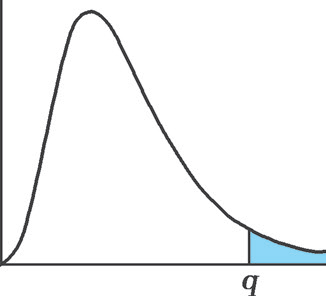
\includegraphics[width=0.25\textwidth]{image/chart5.png}
    \caption*{附表 5 图示}
\end{figure}

\begin{longtable}{c|ccccccccc}
    \hline
    $v$ & \multicolumn{9}{c}{组数 $a$} \\
    & 2 & 3 & 4 & 5 & 6 & 7 & 8 & 9 & 10 \\
    \hline
    \endhead
    5 & 3.64 & 4.60 & 5.22 & 5.67 & 6.03 & 6.33 & 6.58 & 6.80 & 6.99 \\
      & 5.70 & 6.98 & 7.80 & 8.42 & 8.91 & 9.32 & 9.67 & 9.97 & 10.24 \\
    6 & 3.46 & 4.34 & 4.90 & 5.30 & 5.63 & 5.89 & 6.12 & 6.32 & 6.49 \\
      & 5.24 & 6.33 & 7.03 & 7.56 & 7.97 & 8.32 & 8.61 & 8.87 & 9.10 \\
    7 & 3.34 & 4.16 & 4.68 & 5.06 & 5.36 & 5.61 & 5.82 & 6.00 & 6.16 \\
      & 4.95 & 5.92 & 6.54 & 7.01 & 7.37 & 7.68 & 7.94 & 8.17 & 8.37 \\
    8 & 3.26 & 4.04 & 4.53 & 4.89 & 5.17 & 5.40 & 5.60 & 5.77 & 5.92 \\
      & 4.75 & 5.64 & 6.20 & 6.62 & 6.96 & 7.24 & 7.47 & 7.68 & 7.86 \\
    9 & 3.20 & 3.95 & 4.41 & 4.76 & 5.02 & 5.24 & 5.43 & 5.59 & 5.74 \\
      & 4.60 & 5.43 & 5.96 & 6.35 & 6.66 & 6.91 & 7.13 & 7.33 & 7.49 \\
    10 & 3.15 & 3.88 & 4.33 & 4.65 & 4.91 & 5.12 & 5.30 & 5.46 & 5.60 \\
      & 4.48 & 5.27 & 5.77 & 6.14 & 6.43 & 6.67 & 6.87 & 7.05 & 7.21 \\
    12 & 3.08 & 3.77 & 4.20 & 4.51 & 4.75 & 4.95 & 5.12 & 5.27 & 5.39 \\
      & 4.32 & 5.05 & 5.50 & 5.84 & 6.10 & 6.32 & 6.51 & 6.67 & 6.81 \\
    14 & 3.03 & 3.70 & 4.11 & 4.41 & 4.64 & 4.83 & 4.99 & 5.13 & 5.25 \\
      & 4.21 & 4.89 & 5.32 & 5.63 & 5.88 & 6.08 & 6.26 & 6.41 & 6.54 \\
    16 & 3.00 & 3.65 & 4.05 & 4.33 & 4.56 & 4.74 & 4.90 & 5.03 & 5.15 \\
      & 4.13 & 4.79 & 5.19 & 5.49 & 5.72 & 5.92 & 6.08 & 6.22 & 6.35 \\
    18 & 2.97 & 3.61 & 4.00 & 4.28 & 4.49 & 4.67 & 4.82 & 4.96 & 5.07 \\
      & 4.07 & 4.70 & 5.09 & 5.38 & 5.60 & 5.79 & 5.94 & 6.08 & 6.20 \\
    20 & 2.95 & 3.58 & 3.96 & 4.23 & 4.45 & 4.62 & 4.77 & 4.90 & 5.01 \\
      & 4.02 & 4.64 & 5.02 & 5.29 & 5.51 & 5.69 & 5.84 & 5.97 & 6.09 \\
    30 & 2.89 & 3.49 & 3.85 & 4.10 & 4.30 & 4.46 & 4.60 & 4.72 & 4.82 \\
      & 3.89 & 4.45 & 4.80 & 5.05 & 5.24 & 5.40 & 5.54 & 5.65 & 5.76 \\
    40 & 2.86 & 3.44 & 3.79 & 4.04 & 4.23 & 4.39 & 4.52 & 4.63 & 4.73 \\
      & 2.82 & 4.37 & 4.70 & 4.93 & 5.11 & 5.26 & 5.39 & 5.50 & 5.60 \\
    60 & 2.83 & 3.40 & 3.74 & 3.98 & 4.16 & 4.31 & 4.44 & 4.55 & 4.65 \\
      & 3.76 & 4.28 & 4.59 & 4.82 & 4.99 & 5.13 & 5.25 & 5.36 & 5.45 \\
    120 & 2.80 & 3.36 & 3.68 & 3.92 & 4.10 & 4.24 & 4.36 & 4.47 & 4.56 \\
      & 3.70 & 4.20 & 4.50 & 4.71 & 4.87 & 5.01 & 5.12 & 5.21 & 5.30 \\
    $\infty$ & 2.77 & 3.31 & 3.63 & 3.86 & 4.03 & 4.17 & 4.29 & 4.39 & 4.47 \\
      & 3.64 & 4.12 & 4.40 & 4.60 & 4.76 & 4.88 & 4.99 & 5.08 & 5.16 \\
    \hline
\end{longtable}

\newpage

% ==========================================
% 附表 6 百分率的置信区间
% ==========================================
\section{附表 6 百分率的置信区间}
\noindent
上行：95\% 置信区间；下行：99\% 置信区间。

\scriptsize
\begin{longtable}{c|cccccccccccccc}
    \hline
    $n$ & \multicolumn{14}{c}{$x$} \\
    & 0 & 1 & 2 & 3 & 4 & 5 & 6 & 7 & 8 & 9 & 10 & 11 & 12 & 13 \\
    \hline
    \endhead
    1 & 0\textasciitilde98 & & & & & & & & & & & & & \\
      & 0\textasciitilde100 & & & & & & & & & & & & & \\
    2 & 0\textasciitilde84 & 1\textasciitilde99 & & & & & & & & & & & & \\
      & 0\textasciitilde93 & 0\textasciitilde100 & & & & & & & & & & & & \\
    3 & 0\textasciitilde71 & 1\textasciitilde91 & 9\textasciitilde99 & & & & & & & & & & & \\
      & 0\textasciitilde83 & 0\textasciitilde96 & 4\textasciitilde100 & & & & & & & & & & & \\
    4 & 0\textasciitilde60 & 1\textasciitilde81 & 7\textasciitilde93 & & & & & & & & & & & \\
      & 0\textasciitilde73 & 0\textasciitilde89 & 3\textasciitilde97 & & & & & & & & & & & \\
    5 & 0\textasciitilde52 & 1\textasciitilde72 & 5\textasciitilde85 & 15\textasciitilde95 & & & & & & & & & & \\
      & 0\textasciitilde65 & 0\textasciitilde81 & 2\textasciitilde92 & 8\textasciitilde98 & & & & & & & & & & \\
    6 & 0\textasciitilde46 & 0\textasciitilde64 & 4\textasciitilde78 & 12\textasciitilde88 & & & & & & & & & & \\
      & 0\textasciitilde59 & 0\textasciitilde75 & 2\textasciitilde86 & 7\textasciitilde93 & & & & & & & & & & \\
    7 & 0\textasciitilde41 & 0\textasciitilde58 & 4\textasciitilde71 & 10\textasciitilde82 & 18\textasciitilde90 & & & & & & & & & \\
      & 0\textasciitilde53 & 0\textasciitilde68 & 2\textasciitilde80 & 6\textasciitilde88 & 12\textasciitilde94 & & & & & & & & & \\
    8 & 0\textasciitilde37 & 0\textasciitilde53 & 3\textasciitilde65 & 9\textasciitilde76 & 16\textasciitilde84 & & & & & & & & & \\
      & 0\textasciitilde48 & 0\textasciitilde63 & 1\textasciitilde74 & 5\textasciitilde83 & 10\textasciitilde90 & & & & & & & & & \\
    9 & 0\textasciitilde34 & 0\textasciitilde48 & 3\textasciitilde60 & 7\textasciitilde70 & 14\textasciitilde79 & 21\textasciitilde86 & & & & & & & & \\
      & 0\textasciitilde45 & 0\textasciitilde59 & 1\textasciitilde69 & 4\textasciitilde78 & 9\textasciitilde85 & 15\textasciitilde91 & & & & & & & & \\
    10 & 0\textasciitilde31 & 0\textasciitilde45 & 3\textasciitilde56 & 7\textasciitilde65 & 12\textasciitilde74 & 19\textasciitilde81 & & & & & & & & \\
       & 0\textasciitilde41 & 0\textasciitilde54 & 1\textasciitilde65 & 4\textasciitilde74 & 8\textasciitilde81 & 13\textasciitilde87 & & & & & & & & \\
    11 & 0\textasciitilde28 & 0\textasciitilde41 & 2\textasciitilde52 & 6\textasciitilde61 & 11\textasciitilde69 & 17\textasciitilde77 & 23\textasciitilde83 & & & & & & & \\
       & 0\textasciitilde38 & 0\textasciitilde51 & 1\textasciitilde61 & 3\textasciitilde69 & 7\textasciitilde77 & 11\textasciitilde83 & 17\textasciitilde89 & & & & & & & \\
    12 & 0\textasciitilde26 & 0\textasciitilde38 & 2\textasciitilde48 & 5\textasciitilde57 & 10\textasciitilde65 & 15\textasciitilde72 & 21\textasciitilde79 & & & & & & & \\
       & 0\textasciitilde36 & 0\textasciitilde48 & 1\textasciitilde57 & 3\textasciitilde66 & 6\textasciitilde73 & 10\textasciitilde79 & 15\textasciitilde85 & & & & & & & \\
    13 & 0\textasciitilde25 & 0\textasciitilde36 & 2\textasciitilde45 & 5\textasciitilde54 & 9\textasciitilde61 & 14\textasciitilde68 & 19\textasciitilde75 & 25\textasciitilde81 & & & & & & \\
       & 0\textasciitilde34 & 0\textasciitilde45 & 1\textasciitilde54 & 3\textasciitilde62 & 6\textasciitilde69 & 9\textasciitilde76 & 14\textasciitilde81 & 19\textasciitilde86 & & & & & & \\
    14 & 0\textasciitilde23 & 0\textasciitilde34 & 2\textasciitilde43 & 5\textasciitilde51 & 8\textasciitilde58 & 13\textasciitilde65 & 18\textasciitilde71 & 23\textasciitilde77 & & & & & & \\
       & 0\textasciitilde32 & 0\textasciitilde42 & 1\textasciitilde51 & 3\textasciitilde59 & 5\textasciitilde66 & 9\textasciitilde72 & 13\textasciitilde78 & 17\textasciitilde83 & & & & & & \\
    15 & 0\textasciitilde22 & 0\textasciitilde32 & 2\textasciitilde41 & 4\textasciitilde48 & 8\textasciitilde55 & 12\textasciitilde62 & 16\textasciitilde68 & 21\textasciitilde73 & 27\textasciitilde79 & & & & & \\
       & 0\textasciitilde30 & 0\textasciitilde40 & 1\textasciitilde49 & 2\textasciitilde56 & 5\textasciitilde63 & 8\textasciitilde69 & 12\textasciitilde74 & 16\textasciitilde79 & 21\textasciitilde84 & & & & & \\
    16 & 0\textasciitilde21 & 0\textasciitilde30 & 2\textasciitilde38 & 4\textasciitilde46 & 7\textasciitilde52 & 11\textasciitilde59 & 15\textasciitilde65 & 20\textasciitilde70 & 25\textasciitilde75 & & & & & \\
       & 0\textasciitilde28 & 0\textasciitilde38 & 1\textasciitilde46 & 2\textasciitilde53 & 5\textasciitilde60 & 8\textasciitilde66 & 11\textasciitilde71 & 15\textasciitilde76 & 19\textasciitilde81 & & & & & \\
    17 & 0\textasciitilde20 & 0\textasciitilde29 & 2\textasciitilde36 & 4\textasciitilde43 & 7\textasciitilde50 & 10\textasciitilde56 & 14\textasciitilde62 & 18\textasciitilde67 & 23\textasciitilde72 & 28\textasciitilde77 & & & & \\
       & 0\textasciitilde27 & 0\textasciitilde36 & 1\textasciitilde44 & 2\textasciitilde51 & 4\textasciitilde57 & 7\textasciitilde63 & 10\textasciitilde69 & 14\textasciitilde74 & 18\textasciitilde78 & 22\textasciitilde82 & & & & \\
    18 & 0\textasciitilde19 & 0\textasciitilde27 & 1\textasciitilde35 & 4\textasciitilde41 & 6\textasciitilde48 & 10\textasciitilde54 & 13\textasciitilde59 & 17\textasciitilde64 & 22\textasciitilde69 & 26\textasciitilde74 & & & & \\
       & 0\textasciitilde26 & 0\textasciitilde35 & 1\textasciitilde42 & 2\textasciitilde49 & 4\textasciitilde55 & 7\textasciitilde61 & 10\textasciitilde66 & 13\textasciitilde71 & 17\textasciitilde75 & 21\textasciitilde79 & & & & \\
    19 & 0\textasciitilde18 & 0\textasciitilde26 & 1\textasciitilde33 & 3\textasciitilde40 & 6\textasciitilde46 & 9\textasciitilde51 & 13\textasciitilde57 & 16\textasciitilde62 & 20\textasciitilde67 & 24\textasciitilde71 & 29\textasciitilde76 & & & \\
       & 0\textasciitilde24 & 0\textasciitilde33 & 1\textasciitilde40 & 2\textasciitilde47 & 4\textasciitilde53 & 6\textasciitilde58 & 9\textasciitilde63 & 12\textasciitilde68 & 16\textasciitilde73 & 19\textasciitilde77 & 23\textasciitilde81 & & & \\
    20 & 0\textasciitilde17 & 0\textasciitilde25 & 1\textasciitilde32 & 3\textasciitilde38 & 6\textasciitilde44 & 9\textasciitilde49 & 12\textasciitilde54 & 15\textasciitilde59 & 19\textasciitilde64 & 23\textasciitilde69 & 27\textasciitilde73 & & & \\
       & 0\textasciitilde23 & 0\textasciitilde32 & 1\textasciitilde39 & 2\textasciitilde45 & 4\textasciitilde51 & 6\textasciitilde56 & 9\textasciitilde61 & 11\textasciitilde66 & 15\textasciitilde70 & 18\textasciitilde74 & 22\textasciitilde78 & & & \\
    21 & 0\textasciitilde16 & 0\textasciitilde24 & 1\textasciitilde30 & 3\textasciitilde36 & 5\textasciitilde42 & 8\textasciitilde47 & 11\textasciitilde52 & 15\textasciitilde57 & 18\textasciitilde62 & 22\textasciitilde66 & 26\textasciitilde70 & 30\textasciitilde74 & & \\
       & 0\textasciitilde22 & 0\textasciitilde30 & 1\textasciitilde37 & 2\textasciitilde43 & 3\textasciitilde49 & 6\textasciitilde54 & 8\textasciitilde59 & 11\textasciitilde63 & 14\textasciitilde68 & 17\textasciitilde71 & 21\textasciitilde76 & 24\textasciitilde80 & & \\
    22 & 0\textasciitilde15 & 0\textasciitilde23 & 1\textasciitilde29 & 3\textasciitilde35 & 5\textasciitilde40 & 8\textasciitilde45 & 11\textasciitilde50 & 14\textasciitilde55 & 17\textasciitilde59 & 21\textasciitilde64 & 24\textasciitilde68 & 28\textasciitilde72 & & \\
       & 0\textasciitilde21 & 0\textasciitilde29 & 1\textasciitilde36 & 2\textasciitilde42 & 3\textasciitilde47 & 5\textasciitilde52 & 8\textasciitilde57 & 10\textasciitilde61 & 13\textasciitilde66 & 16\textasciitilde70 & 20\textasciitilde73 & 23\textasciitilde77 & & \\
    23 & 0\textasciitilde15 & 0\textasciitilde22 & 1\textasciitilde28 & 3\textasciitilde34 & 5\textasciitilde39 & 8\textasciitilde44 & 10\textasciitilde48 & 13\textasciitilde53 & 16\textasciitilde57 & 20\textasciitilde62 & 23\textasciitilde66 & 27\textasciitilde69 & 31\textasciitilde73 & \\
       & 0\textasciitilde21 & 0\textasciitilde28 & 1\textasciitilde35 & 2\textasciitilde40 & 3\textasciitilde45 & 5\textasciitilde50 & 7\textasciitilde55 & 10\textasciitilde59 & 13\textasciitilde63 & 15\textasciitilde67 & 19\textasciitilde71 & 22\textasciitilde75 & 25\textasciitilde78 & \\
    24 & 0\textasciitilde14 & 0\textasciitilde21 & 1\textasciitilde27 & 3\textasciitilde32 & 5\textasciitilde37 & 7\textasciitilde42 & 10\textasciitilde47 & 13\textasciitilde51 & 16\textasciitilde55 & 19\textasciitilde59 & 22\textasciitilde63 & 26\textasciitilde67 & 29\textasciitilde71 & \\
       & 0\textasciitilde20 & 0\textasciitilde27 & 0\textasciitilde33 & 2\textasciitilde39 & 3\textasciitilde44 & 5\textasciitilde49 & 7\textasciitilde53 & 9\textasciitilde57 & 12\textasciitilde61 & 15\textasciitilde65 & 18\textasciitilde69 & 21\textasciitilde73 & 24\textasciitilde76 & \\
    25 & 0\textasciitilde14 & 0\textasciitilde20 & 1\textasciitilde26 & 3\textasciitilde31 & 5\textasciitilde36 & 7\textasciitilde41 & 9\textasciitilde45 & 12\textasciitilde49 & 15\textasciitilde54 & 18\textasciitilde58 & 21\textasciitilde61 & 24\textasciitilde65 & 28\textasciitilde69 & 31\textasciitilde72 \\
       & 0\textasciitilde19 & 0\textasciitilde26 & 0\textasciitilde32 & 1\textasciitilde37 & 3\textasciitilde42 & 5\textasciitilde47 & 7\textasciitilde51 & 9\textasciitilde56 & 11\textasciitilde60 & 14\textasciitilde63 & 17\textasciitilde67 & 20\textasciitilde71 & 23\textasciitilde74 & 26\textasciitilde77 \\
    26 & 0\textasciitilde13 & 0\textasciitilde20 & 1\textasciitilde25 & 2\textasciitilde30 & 4\textasciitilde35 & 7\textasciitilde39 & 9\textasciitilde44 & 12\textasciitilde48 & 14\textasciitilde52 & 17\textasciitilde56 & 20\textasciitilde60 & 23\textasciitilde63 & 27\textasciitilde67 & 30\textasciitilde70 \\
       & 0\textasciitilde18 & 0\textasciitilde25 & 0\textasciitilde31 & 1\textasciitilde36 & 3\textasciitilde41 & 4\textasciitilde46 & 6\textasciitilde50 & 9\textasciitilde54 & 11\textasciitilde58 & 13\textasciitilde62 & 16\textasciitilde65 & 19\textasciitilde69 & 22\textasciitilde72 & 25\textasciitilde75 \\
    27 & 0\textasciitilde13 & 0\textasciitilde19 & 1\textasciitilde24 & 2\textasciitilde29 & 4\textasciitilde34 & 6\textasciitilde38 & 9\textasciitilde42 & 11\textasciitilde46 & 14\textasciitilde50 & 17\textasciitilde54 & 19\textasciitilde58 & 22\textasciitilde61 & 26\textasciitilde65 & 29\textasciitilde68 \\
       & 0\textasciitilde18 & 0\textasciitilde25 & 0\textasciitilde30 & 1\textasciitilde35 & 3\textasciitilde40 & 4\textasciitilde44 & 6\textasciitilde48 & 8\textasciitilde52 & 10\textasciitilde56 & 13\textasciitilde60 & 15\textasciitilde63 & 18\textasciitilde67 & 21\textasciitilde70 & 24\textasciitilde73 \\
    28 & 0\textasciitilde12 & 0\textasciitilde18 & 1\textasciitilde24 & 2\textasciitilde28 & 4\textasciitilde33 & 6\textasciitilde37 & 8\textasciitilde41 & 11\textasciitilde45 & 13\textasciitilde49 & 16\textasciitilde52 & 19\textasciitilde56 & 22\textasciitilde59 & 25\textasciitilde63 & 28\textasciitilde66 \\
       & 0\textasciitilde17 & 0\textasciitilde24 & 0\textasciitilde29 & 1\textasciitilde34 & 3\textasciitilde39 & 4\textasciitilde43 & 6\textasciitilde47 & 8\textasciitilde51 & 10\textasciitilde55 & 12\textasciitilde58 & 15\textasciitilde62 & 17\textasciitilde65 & 20\textasciitilde68 & 23\textasciitilde71 \\
    29 & 0\textasciitilde12 & 0\textasciitilde18 & 1\textasciitilde23 & 2\textasciitilde27 & 4\textasciitilde32 & 6\textasciitilde36 & 8\textasciitilde40 & 10\textasciitilde44 & 13\textasciitilde47 & 15\textasciitilde51 & 18\textasciitilde54 & 21\textasciitilde58 & 24\textasciitilde61 & 26\textasciitilde64 \\
       & 0\textasciitilde17 & 0\textasciitilde23 & 0\textasciitilde28 & 1\textasciitilde33 & 2\textasciitilde37 & 4\textasciitilde42 & 6\textasciitilde46 & 8\textasciitilde49 & 10\textasciitilde53 & 12\textasciitilde57 & 14\textasciitilde60 & 17\textasciitilde63 & 19\textasciitilde66 & 22\textasciitilde70 \\
    30 & 0\textasciitilde12 & 0\textasciitilde17 & 1\textasciitilde22 & 2\textasciitilde27 & 4\textasciitilde31 & 6\textasciitilde35 & 8\textasciitilde39 & 10\textasciitilde42 & 12\textasciitilde46 & 15\textasciitilde49 & 17\textasciitilde53 & 20\textasciitilde56 & 23\textasciitilde59 & 26\textasciitilde63 \\
       & 0\textasciitilde16 & 0\textasciitilde22 & 0\textasciitilde27 & 1\textasciitilde32 & 2\textasciitilde36 & 4\textasciitilde40 & 5\textasciitilde44 & 7\textasciitilde48 & 9\textasciitilde52 & 11\textasciitilde55 & 14\textasciitilde58 & 16\textasciitilde62 & 19\textasciitilde65 & 21\textasciitilde68 \\
    31 & 0\textasciitilde11 & 0\textasciitilde17 & 1\textasciitilde22 & 2\textasciitilde26 & 4\textasciitilde30 & 6\textasciitilde34 & 8\textasciitilde38 & 10\textasciitilde41 & 12\textasciitilde45 & 14\textasciitilde48 & 17\textasciitilde51 & 19\textasciitilde55 & 22\textasciitilde58 & 25\textasciitilde61 \\
       & 0\textasciitilde16 & 0\textasciitilde22 & 0\textasciitilde27 & 1\textasciitilde31 & 2\textasciitilde35 & 4\textasciitilde39 & 5\textasciitilde43 & 7\textasciitilde47 & 9\textasciitilde50 & 11\textasciitilde54 & 13\textasciitilde57 & 16\textasciitilde60 & 18\textasciitilde63 & 20\textasciitilde66 \\
    32 & 0\textasciitilde11 & 0\textasciitilde16 & 1\textasciitilde21 & 2\textasciitilde25 & 4\textasciitilde29 & 5\textasciitilde33 & 7\textasciitilde36 & 9\textasciitilde40 & 12\textasciitilde43 & 14\textasciitilde47 & 16\textasciitilde50 & 19\textasciitilde53 & 21\textasciitilde56 & 24\textasciitilde59 \\
       & 0\textasciitilde15 & 0\textasciitilde21 & 0\textasciitilde26 & 1\textasciitilde30 & 2\textasciitilde34 & 4\textasciitilde38 & 5\textasciitilde42 & 7\textasciitilde46 & 9\textasciitilde49 & 11\textasciitilde52 & 13\textasciitilde56 & 15\textasciitilde59 & 17\textasciitilde62 & 20\textasciitilde65 \\
    33 & 0\textasciitilde11 & 0\textasciitilde15 & 1\textasciitilde20 & 2\textasciitilde24 & 3\textasciitilde28 & 5\textasciitilde32 & 7\textasciitilde36 & 9\textasciitilde39 & 11\textasciitilde42 & 13\textasciitilde46 & 16\textasciitilde49 & 18\textasciitilde52 & 20\textasciitilde55 & 23\textasciitilde58 \\
       & 0\textasciitilde15 & 0\textasciitilde20 & 0\textasciitilde25 & 1\textasciitilde30 & 2\textasciitilde34 & 3\textasciitilde37 & 5\textasciitilde41 & 7\textasciitilde44 & 8\textasciitilde48 & 10\textasciitilde51 & 12\textasciitilde54 & 14\textasciitilde57 & 17\textasciitilde60 & 19\textasciitilde63 \\
    34 & 0\textasciitilde10 & 0\textasciitilde15 & 1\textasciitilde19 & 2\textasciitilde23 & 3\textasciitilde28 & 5\textasciitilde31 & 7\textasciitilde35 & 9\textasciitilde38 & 11\textasciitilde41 & 13\textasciitilde44 & 15\textasciitilde48 & 17\textasciitilde51 & 20\textasciitilde54 & 22\textasciitilde56 \\
       & 0\textasciitilde14 & 0\textasciitilde20 & 0\textasciitilde25 & 1\textasciitilde29 & 2\textasciitilde33 & 3\textasciitilde36 & 5\textasciitilde40 & 6\textasciitilde43 & 8\textasciitilde47 & 10\textasciitilde50 & 12\textasciitilde53 & 14\textasciitilde56 & 16\textasciitilde59 & 18\textasciitilde62 \\
    35 & 0\textasciitilde10 & 0\textasciitilde15 & 1\textasciitilde19 & 2\textasciitilde23 & 3\textasciitilde27 & 5\textasciitilde30 & 7\textasciitilde34 & 8\textasciitilde37 & 10\textasciitilde40 & 13\textasciitilde43 & 15\textasciitilde46 & 17\textasciitilde49 & 19\textasciitilde52 & 22\textasciitilde55 \\
       & 0\textasciitilde14 & 0\textasciitilde20 & 0\textasciitilde24 & 1\textasciitilde28 & 2\textasciitilde32 & 3\textasciitilde35 & 5\textasciitilde39 & 6\textasciitilde42 & 8\textasciitilde45 & 10\textasciitilde49 & 12\textasciitilde52 & 14\textasciitilde55 & 16\textasciitilde57 & 18\textasciitilde60 \\
    36 & 0\textasciitilde10 & 0\textasciitilde15 & 1\textasciitilde18 & 2\textasciitilde22 & 3\textasciitilde26 & 5\textasciitilde29 & 6\textasciitilde33 & 8\textasciitilde36 & 10\textasciitilde39 & 12\textasciitilde42 & 14\textasciitilde45 & 16\textasciitilde48 & 19\textasciitilde51 & 21\textasciitilde54 \\
       & 0\textasciitilde14 & 0\textasciitilde19 & 0\textasciitilde23 & 1\textasciitilde27 & 2\textasciitilde31 & 3\textasciitilde35 & 5\textasciitilde38 & 6\textasciitilde41 & 8\textasciitilde44 & 9\textasciitilde47 & 11\textasciitilde50 & 13\textasciitilde53 & 15\textasciitilde56 & 17\textasciitilde59 \\
    37 & 0\textasciitilde10 & 0\textasciitilde14 & 1\textasciitilde18 & 2\textasciitilde22 & 3\textasciitilde25 & 5\textasciitilde28 & 6\textasciitilde32 & 8\textasciitilde35 & 10\textasciitilde38 & 12\textasciitilde41 & 14\textasciitilde44 & 16\textasciitilde47 & 18\textasciitilde50 & 20\textasciitilde53 \\
       & 0\textasciitilde13 & 0\textasciitilde18 & 0\textasciitilde23 & 1\textasciitilde27 & 2\textasciitilde30 & 3\textasciitilde34 & 4\textasciitilde37 & 6\textasciitilde40 & 7\textasciitilde43 & 9\textasciitilde46 & 11\textasciitilde49 & 13\textasciitilde52 & 15\textasciitilde55 & 17\textasciitilde58 \\
    38 & 0\textasciitilde10 & 0\textasciitilde14 & 1\textasciitilde18 & 2\textasciitilde21 & 3\textasciitilde25 & 5\textasciitilde28 & 6\textasciitilde32 & 8\textasciitilde34 & 10\textasciitilde37 & 11\textasciitilde40 & 13\textasciitilde43 & 15\textasciitilde46 & 18\textasciitilde49 & 20\textasciitilde51 \\
       & 0\textasciitilde13 & 0\textasciitilde18 & 0\textasciitilde22 & 1\textasciitilde26 & 2\textasciitilde30 & 3\textasciitilde33 & 4\textasciitilde36 & 6\textasciitilde39 & 7\textasciitilde42 & 9\textasciitilde45 & 11\textasciitilde48 & 12\textasciitilde51 & 14\textasciitilde54 & 16\textasciitilde56 \\
    39 & 0\textasciitilde9 & 0\textasciitilde14 & 1\textasciitilde17 & 2\textasciitilde21 & 3\textasciitilde24 & 4\textasciitilde27 & 6\textasciitilde31 & 8\textasciitilde33 & 9\textasciitilde36 & 11\textasciitilde39 & 13\textasciitilde42 & 15\textasciitilde45 & 17\textasciitilde48 & 19\textasciitilde50 \\
       & 0\textasciitilde13 & 0\textasciitilde18 & 0\textasciitilde21 & 1\textasciitilde25 & 2\textasciitilde29 & 3\textasciitilde32 & 4\textasciitilde35 & 6\textasciitilde38 & 7\textasciitilde41 & 9\textasciitilde44 & 10\textasciitilde47 & 12\textasciitilde50 & 14\textasciitilde53 & 16\textasciitilde55 \\
    40 & 0\textasciitilde9 & 0\textasciitilde13 & 1\textasciitilde17 & 2\textasciitilde21 & 3\textasciitilde24 & 4\textasciitilde27 & 6\textasciitilde30 & 8\textasciitilde33 & 9\textasciitilde35 & 11\textasciitilde38 & 13\textasciitilde41 & 15\textasciitilde44 & 17\textasciitilde47 & 19\textasciitilde49 \\
       & 0\textasciitilde12 & 0\textasciitilde17 & 0\textasciitilde21 & 1\textasciitilde25 & 2\textasciitilde28 & 3\textasciitilde32 & 4\textasciitilde35 & 5\textasciitilde38 & 7\textasciitilde40 & 9\textasciitilde43 & 10\textasciitilde46 & 12\textasciitilde49 & 13\textasciitilde52 & 15\textasciitilde54 \\
    41 & 0\textasciitilde9 & 0\textasciitilde13 & 1\textasciitilde17 & 2\textasciitilde20 & 3\textasciitilde23 & 4\textasciitilde26 & 6\textasciitilde29 & 7\textasciitilde32 & 9\textasciitilde35 & 11\textasciitilde37 & 12\textasciitilde40 & 14\textasciitilde43 & 16\textasciitilde46 & 18\textasciitilde48 \\
       & 0\textasciitilde12 & 0\textasciitilde17 & 0\textasciitilde21 & 1\textasciitilde24 & 2\textasciitilde28 & 3\textasciitilde31 & 4\textasciitilde34 & 5\textasciitilde37 & 7\textasciitilde40 & 8\textasciitilde42 & 10\textasciitilde45 & 11\textasciitilde48 & 13\textasciitilde50 & 15\textasciitilde53 \\
    42 & 0\textasciitilde9 & 0\textasciitilde13 & 1\textasciitilde16 & 2\textasciitilde20 & 3\textasciitilde23 & 4\textasciitilde26 & 6\textasciitilde28 & 7\textasciitilde31 & 9\textasciitilde34 & 10\textasciitilde37 & 12\textasciitilde39 & 14\textasciitilde42 & 16\textasciitilde45 & 18\textasciitilde47 \\
       & 0\textasciitilde12 & 0\textasciitilde17 & 0\textasciitilde20 & 1\textasciitilde24 & 2\textasciitilde27 & 3\textasciitilde30 & 4\textasciitilde33 & 5\textasciitilde36 & 7\textasciitilde39 & 8\textasciitilde42 & 9\textasciitilde44 & 11\textasciitilde47 & 13\textasciitilde49 & 15\textasciitilde52 \\
    43 & 0\textasciitilde9 & 0\textasciitilde12 & 1\textasciitilde16 & 2\textasciitilde19 & 3\textasciitilde23 & 4\textasciitilde25 & 5\textasciitilde28 & 7\textasciitilde31 & 8\textasciitilde33 & 10\textasciitilde36 & 12\textasciitilde39 & 14\textasciitilde41 & 15\textasciitilde44 & 17\textasciitilde46 \\
       & 0\textasciitilde12 & 0\textasciitilde16 & 0\textasciitilde20 & 1\textasciitilde23 & 2\textasciitilde26 & 3\textasciitilde30 & 4\textasciitilde33 & 5\textasciitilde35 & 6\textasciitilde38 & 8\textasciitilde41 & 9\textasciitilde43 & 11\textasciitilde46 & 13\textasciitilde49 & 14\textasciitilde51 \\
    44 & 0\textasciitilde9 & 0\textasciitilde12 & 1\textasciitilde15 & 2\textasciitilde19 & 3\textasciitilde22 & 4\textasciitilde25 & 5\textasciitilde28 & 7\textasciitilde30 & 8\textasciitilde33 & 10\textasciitilde35 & 11\textasciitilde38 & 13\textasciitilde40 & 15\textasciitilde43 & 17\textasciitilde45 \\
       & 0\textasciitilde11 & 0\textasciitilde16 & 0\textasciitilde19 & 1\textasciitilde23 & 2\textasciitilde26 & 3\textasciitilde29 & 4\textasciitilde32 & 5\textasciitilde35 & 6\textasciitilde37 & 8\textasciitilde40 & 9\textasciitilde42 & 11\textasciitilde45 & 12\textasciitilde47 & 14\textasciitilde50 \\
    45 & 0\textasciitilde8 & 0\textasciitilde12 & 1\textasciitilde15 & 2\textasciitilde18 & 3\textasciitilde21 & 4\textasciitilde24 & 5\textasciitilde27 & 7\textasciitilde30 & 8\textasciitilde32 & 9\textasciitilde34 & 11\textasciitilde37 & 13\textasciitilde39 & 15\textasciitilde42 & 16\textasciitilde44 \\
       & 0\textasciitilde11 & 0\textasciitilde15 & 0\textasciitilde19 & 1\textasciitilde22 & 2\textasciitilde25 & 3\textasciitilde28 & 4\textasciitilde31 & 5\textasciitilde34 & 6\textasciitilde37 & 8\textasciitilde39 & 9\textasciitilde42 & 10\textasciitilde44 & 12\textasciitilde47 & 14\textasciitilde49 \\
    46 & 0\textasciitilde8 & 0\textasciitilde12 & 1\textasciitilde15 & 2\textasciitilde18 & 3\textasciitilde21 & 4\textasciitilde24 & 5\textasciitilde26 & 7\textasciitilde29 & 8\textasciitilde31 & 9\textasciitilde34 & 11\textasciitilde36 & 13\textasciitilde39 & 14\textasciitilde41 & 16\textasciitilde43 \\
       & 0\textasciitilde11 & 0\textasciitilde15 & 0\textasciitilde19 & 1\textasciitilde22 & 2\textasciitilde25 & 3\textasciitilde28 & 4\textasciitilde31 & 5\textasciitilde33 & 6\textasciitilde36 & 7\textasciitilde39 & 9\textasciitilde41 & 10\textasciitilde43 & 12\textasciitilde46 & 13\textasciitilde48 \\
    47 & 0\textasciitilde8 & 0\textasciitilde12 & 1\textasciitilde15 & 2\textasciitilde17 & 3\textasciitilde20 & 4\textasciitilde23 & 5\textasciitilde26 & 6\textasciitilde28 & 8\textasciitilde31 & 9\textasciitilde34 & 11\textasciitilde36 & 12\textasciitilde38 & 14\textasciitilde40 & 16\textasciitilde43 \\
       & 0\textasciitilde11 & 0\textasciitilde15 & 0\textasciitilde18 & 1\textasciitilde21 & 2\textasciitilde24 & 2\textasciitilde27 & 3\textasciitilde30 & 5\textasciitilde33 & 6\textasciitilde35 & 7\textasciitilde38 & 9\textasciitilde40 & 10\textasciitilde42 & 11\textasciitilde45 & 13\textasciitilde47 \\
    48 & 0\textasciitilde8 & 0\textasciitilde11 & 1\textasciitilde14 & 2\textasciitilde17 & 3\textasciitilde20 & 4\textasciitilde22 & 5\textasciitilde25 & 6\textasciitilde28 & 8\textasciitilde30 & 9\textasciitilde33 & 11\textasciitilde35 & 12\textasciitilde37 & 14\textasciitilde39 & 15\textasciitilde42 \\
       & 0\textasciitilde10 & 0\textasciitilde14 & 0\textasciitilde18 & 1\textasciitilde21 & 2\textasciitilde24 & 2\textasciitilde27 & 3\textasciitilde29 & 5\textasciitilde32 & 6\textasciitilde35 & 7\textasciitilde37 & 8\textasciitilde40 & 10\textasciitilde42 & 11\textasciitilde44 & 13\textasciitilde47 \\
    49 & 0\textasciitilde8 & 0\textasciitilde11 & 1\textasciitilde14 & 2\textasciitilde17 & 2\textasciitilde20 & 4\textasciitilde22 & 5\textasciitilde25 & 6\textasciitilde27 & 7\textasciitilde30 & 9\textasciitilde32 & 10\textasciitilde35 & 12\textasciitilde37 & 13\textasciitilde39 & 15\textasciitilde41 \\
       & 0\textasciitilde10 & 0\textasciitilde14 & 0\textasciitilde17 & 1\textasciitilde20 & 1\textasciitilde24 & 2\textasciitilde26 & 3\textasciitilde29 & 4\textasciitilde32 & 6\textasciitilde34 & 7\textasciitilde36 & 8\textasciitilde39 & 9\textasciitilde41 & 11\textasciitilde44 & 12\textasciitilde46 \\
    50 & 0\textasciitilde7 & 0\textasciitilde11 & 1\textasciitilde14 & 2\textasciitilde17 & 2\textasciitilde19 & 3\textasciitilde22 & 5\textasciitilde24 & 6\textasciitilde26 & 7\textasciitilde29 & 9\textasciitilde31 & 10\textasciitilde34 & 11\textasciitilde36 & 13\textasciitilde38 & 15\textasciitilde41 \\
       & 0\textasciitilde10 & 0\textasciitilde14 & 0\textasciitilde17 & 1\textasciitilde20 & 1\textasciitilde23 & 2\textasciitilde26 & 3\textasciitilde28 & 4\textasciitilde31 & 5\textasciitilde33 & 7\textasciitilde36 & 8\textasciitilde38 & 9\textasciitilde40 & 11\textasciitilde43 & 12\textasciitilde45 \\
    \hline
\end{longtable}
\normalsize

\newpage

% ==========================================
% 附表 7 χ2 分布界值表
% ==========================================
\section{附表 7 $\chi^2$ 分布界值表}
\begin{figure}[htbp]
    \raggedleft
    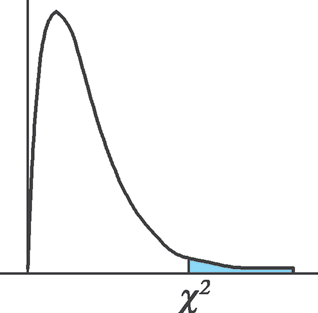
\includegraphics[width=0.25\textwidth]{image/chart7.png}
    \caption*{附表 7 图示}
\end{figure}

\begin{longtable}{c|cccccccccc}
    \hline
    自由度 & \multicolumn{10}{c}{概率 $P$（右侧尾部面积）} \\
    $v$ & 0.995 & 0.990 & 0.975 & 0.950 & 0.900 & 0.750 & 0.500 & 0.250 & 0.100 & 0.050 \\
    \hline
    \endhead
    1 & & & 0.001 & 0.004 & 0.016 & 0.102 & 0.455 & 1.323 & 2.706 & 3.841 \\
    2 & 0.010 & 0.020 & 0.051 & 0.103 & 0.211 & 0.575 & 1.386 & 2.773 & 4.605 & 5.991 \\
    3 & 0.072 & 0.115 & 0.216 & 0.352 & 0.584 & 1.213 & 2.366 & 4.108 & 6.251 & 7.815 \\
    4 & 0.207 & 0.297 & 0.484 & 0.711 & 1.064 & 1.923 & 3.357 & 5.385 & 7.779 & 9.488 \\
    5 & 0.412 & 0.554 & 0.831 & 1.145 & 1.610 & 2.675 & 4.351 & 6.626 & 9.236 & 11.070 \\
    6 & 0.676 & 0.872 & 1.237 & 1.635 & 2.204 & 3.455 & 5.348 & 7.841 & 10.645 & 12.592 \\
    7 & 0.989 & 1.239 & 1.690 & 2.167 & 2.833 & 4.255 & 6.346 & 9.037 & 12.017 & 14.067 \\
    8 & 1.344 & 1.646 & 2.180 & 2.733 & 3.490 & 5.071 & 7.344 & 10.219 & 13.362 & 15.507 \\
    9 & 1.735 & 2.088 & 2.700 & 3.325 & 4.168 & 5.899 & 8.343 & 11.389 & 14.684 & 16.919 \\
    10 & 2.156 & 2.558 & 3.247 & 3.940 & 4.865 & 6.737 & 9.342 & 12.549 & 15.987 & 18.307 \\
    11 & 2.603 & 3.053 & 3.816 & 4.575 & 5.578 & 7.584 & 10.341 & 13.701 & 17.275 & 19.675 \\
    12 & 3.074 & 3.571 & 4.404 & 5.226 & 6.304 & 8.438 & 11.340 & 14.845 & 18.549 & 21.026 \\
    13 & 3.565 & 4.107 & 5.009 & 5.892 & 7.042 & 9.299 & 12.340 & 15.984 & 19.812 & 22.362 \\
    14 & 4.075 & 4.660 & 5.629 & 6.571 & 7.790 & 10.165 & 13.339 & 17.117 & 21.064 & 23.685 \\
    15 & 4.601 & 5.229 & 6.262 & 7.261 & 8.547 & 11.037 & 14.339 & 18.245 & 22.307 & 24.996 \\
    20 & 7.434 & 8.260 & 9.591 & 10.851 & 12.443 & 15.452 & 19.337 & 23.828 & 28.412 & 31.410 \\
    30 & 13.787 & 14.953 & 16.791 & 18.493 & 20.599 & 24.478 & 29.336 & 34.800 & 40.256 & 43.773 \\
    40 & 20.707 & 22.164 & 24.433 & 26.509 & 29.051 & 33.660 & 39.335 & 45.616 & 51.805 & 55.758 \\
    50 & 27.991 & 29.707 & 32.357 & 34.764 & 37.689 & 42.942 & 49.335 & 56.334 & 63.167 & 67.505 \\
    100 & 67.328 & 70.065 & 74.222 & 77.929 & 82.358 & 90.133 & 99.334 & 109.141 & 118.498 & 124.342 \\
    \hline
\end{longtable}

\newpage

% ==========================================
% 附表 8 T 界值表
% ==========================================
\section{附表 8 $T$ 界值表（配对比较的符号秩和检验用）}
\begin{longtable}{c|ccc}
    \hline
    $n$ & \multicolumn{3}{c}{概率 $P$} \\
    & 单侧 0.025 / 双侧 0.05 & 单侧 0.01 / 双侧 0.02 & 单侧 0.005 / 双侧 0.01 \\
    \hline
    \endhead
    5  & — & — & — \\
    6  & 0 & — & — \\
    7  & 2 & 0 & — \\
    8  & 3 & 1 & 0 \\
    9  & 5 & 3 & 1 \\
    10 & 8 & 5 & 3 \\
    11 & 10 & 7 & 5 \\
    12 & 13 & 9 & 7 \\
    13 & 17 & 12 & 9 \\
    14 & 21 & 15 & 12 \\
    15 & 25 & 19 & 15 \\
    16 & 29 & 23 & 19 \\
    17 & 34 & 27 & 23 \\
    18 & 40 & 32 & 27 \\
    19 & 46 & 37 & 32 \\
    20 & 52 & 43 & 37 \\
    21 & 58 & 49 & 42 \\
    22 & 65 & 55 & 48 \\
    23 & 73 & 62 & 54 \\
    24 & 81 & 69 & 61 \\
    25 & 89 & 76 & 68 \\
    30 & 137 & 120 & 109 \\
    40 & 264 & 238 & 220 \\
    50 & 434 & 397 & 373 \\
    \hline
\end{longtable}

\newpage

% ==========================================
% 附表 9 T 界值表（秩和检验）
% ==========================================
\section{附表 9 $T$ 界值表（两样本比较的秩和检验用）}

\begin{figure}[htbp]
    \centering
    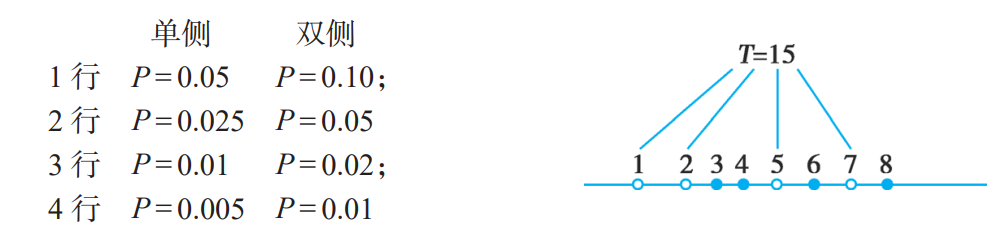
\includegraphics[width=0.5\textwidth]{image/chart9.png}
    \caption*{附表 9 图示}
\end{figure}

\footnotesize
\begin{longtable}{c|ccccccccccc}
    \hline
    $n_1$ & \multicolumn{11}{c}{$n_2 - n_1$} \\
    (较小 $n$) & 0 & 1 & 2 & 3 & 4 & 5 & 6 & 7 & 8 & 9 & 10 \\
    \hline
    \endhead
    2 & & & 3\textasciitilde13 & 3\textasciitilde15 & 3\textasciitilde17 & 4\textasciitilde18 & 4\textasciitilde20 & 4\textasciitilde22 & 4\textasciitilde24 & 5\textasciitilde25 \\
      & & & & & & & 3\textasciitilde19 & 3\textasciitilde21 & 3\textasciitilde23 & 3\textasciitilde25 & 4\textasciitilde26 \\
    3 & 6\textasciitilde15 & 6\textasciitilde18 & 7\textasciitilde20 & 8\textasciitilde22 & 8\textasciitilde25 & 9\textasciitilde27 & 10\textasciitilde29 & 10\textasciitilde32 & 11\textasciitilde34 & 11\textasciitilde37 & 12\textasciitilde39 \\
      & & 6\textasciitilde21 & 7\textasciitilde23 & 7\textasciitilde26 & 8\textasciitilde28 & 8\textasciitilde31 & 9\textasciitilde33 & 9\textasciitilde36 & 10\textasciitilde38 & 10\textasciitilde41 \\
    4 & 11\textasciitilde25 & 12\textasciitilde28 & 13\textasciitilde31 & 14\textasciitilde34 & 15\textasciitilde37 & 16\textasciitilde40 & 17\textasciitilde43 & 18\textasciitilde46 & 19\textasciitilde49 & 20\textasciitilde52 & 21\textasciitilde55 \\
      & 10\textasciitilde26 & 11\textasciitilde29 & 12\textasciitilde32 & 13\textasciitilde35 & 14\textasciitilde38 & 14\textasciitilde42 & 15\textasciitilde45 & 16\textasciitilde48 & 17\textasciitilde51 & 18\textasciitilde54 & 19\textasciitilde57 \\
    5 & 19\textasciitilde36 & 20\textasciitilde40 & 21\textasciitilde44 & 23\textasciitilde47 & 24\textasciitilde51 & 26\textasciitilde54 & 27\textasciitilde58 & 28\textasciitilde62 & 30\textasciitilde65 & 31\textasciitilde69 & 33\textasciitilde72 \\
      & 17\textasciitilde38 & 18\textasciitilde42 & 20\textasciitilde45 & 21\textasciitilde49 & 22\textasciitilde53 & 23\textasciitilde57 & 24\textasciitilde61 & 26\textasciitilde64 & 27\textasciitilde68 & 28\textasciitilde72 & 29\textasciitilde76 \\
    6 & 28\textasciitilde50 & 29\textasciitilde55 & 31\textasciitilde59 & 33\textasciitilde63 & 35\textasciitilde67 & 37\textasciitilde71 & 38\textasciitilde76 & 40\textasciitilde80 & 42\textasciitilde84 & 44\textasciitilde88 & 46\textasciitilde92 \\
      & 26\textasciitilde52 & 27\textasciitilde57 & 29\textasciitilde61 & 31\textasciitilde65 & 32\textasciitilde70 & 34\textasciitilde74 & 35\textasciitilde79 & 37\textasciitilde83 & 38\textasciitilde88 & 40\textasciitilde92 & 42\textasciitilde96 \\
    7 & 39\textasciitilde66 & 41\textasciitilde71 & 43\textasciitilde76 & 45\textasciitilde81 & 47\textasciitilde86 & 49\textasciitilde91 & 52\textasciitilde95 & 54\textasciitilde100 & 46\textasciitilde105 & 58\textasciitilde110 & 61\textasciitilde114 \\
      & 36\textasciitilde69 & 38\textasciitilde74 & 40\textasciitilde79 & 42\textasciitilde84 & 44\textasciitilde89 & 46\textasciitilde94 & 48\textasciitilde99 & 50\textasciitilde104 & 52\textasciitilde109 & 54\textasciitilde114 & 56\textasciitilde119 \\
    8 & 51\textasciitilde85 & 54\textasciitilde90 & 56\textasciitilde96 & 59\textasciitilde101 & 62\textasciitilde106 & 64\textasciitilde112 & 67\textasciitilde117 & 69\textasciitilde123 & 72\textasciitilde128 & 75\textasciitilde133 & 77\textasciitilde139 \\
      & 49\textasciitilde87 & 51\textasciitilde93 & 53\textasciitilde99 & 55\textasciitilde105 & 58\textasciitilde110 & 60\textasciitilde116 & 62\textasciitilde122 & 65\textasciitilde127 & 67\textasciitilde133 & 70\textasciitilde138 & 72\textasciitilde144 \\
    9 & 66\textasciitilde105 & 69\textasciitilde111 & 72\textasciitilde117 & 75\textasciitilde123 & 78\textasciitilde129 & 81\textasciitilde135 & 84\textasciitilde141 & 87\textasciitilde147 & 90\textasciitilde153 & 93\textasciitilde159 & 96\textasciitilde165 \\
      & 62\textasciitilde109 & 65\textasciitilde115 & 68\textasciitilde121 & 71\textasciitilde127 & 73\textasciitilde134 & 76\textasciitilde140 & 79\textasciitilde146 & 82\textasciitilde152 & 84\textasciitilde159 & 87\textasciitilde165 & 90\textasciitilde171 \\
    10 & 82\textasciitilde128 & 86\textasciitilde134 & 89\textasciitilde141 & 92\textasciitilde148 & 96\textasciitilde154 & 99\textasciitilde161 & 103\textasciitilde167 & 106\textasciitilde174 & 110\textasciitilde180 & 113\textasciitilde187 & 117\textasciitilde193 \\
       & 78\textasciitilde132 & 81\textasciitilde139 & 84\textasciitilde146 & 88\textasciitilde152 & 91\textasciitilde159 & 94\textasciitilde166 & 97\textasciitilde173 & 100\textasciitilde180 & 103\textasciitilde187 & 107\textasciitilde103 & 110\textasciitilde200 \\
    \hline
\end{longtable}
\normalsize

\newpage



% ==========================================
% 附表 10 H 界值表
% ==========================================
\section{附表 10 $H$ 界值表（三样本比较的秩和检验用）}

\vspace{0.5em}
\centering
\begin{longtable}{p{0.08\textwidth} p{0.12\textwidth} p{0.12\textwidth} p{0.12\textwidth} p{0.18\textwidth} p{0.18\textwidth}}
    \hline
    $N$ & $n_1$ & $n_2$ & $n_3$ & \multicolumn{2}{c}{$P$} \\
    \cline{5-6}
    & & & & 0.05 & 0.01 \\
    \hline
    \endhead
    
    % N = 7
    7 & 3 & 2 & 2 & 4.71 & \\
    & 3 & 3 & 1 & 5.14 & \\
    
    % N = 8
    8 & 3 & 3 & 2 & 5.36 & \\
    & 4 & 2 & 2 & 5.33 & \\
    & 4 & 3 & 1 & 5.21 & \\
    & 5 & 2 & 1 & 5.00 & \\
    
    % N = 9
    9 & 3 & 3 & 3 & 5.60 & 7.20 \\
    & 4 & 3 & 2 & 5.44 & 6.44 \\
    & 4 & 4 & 1 & 4.97 & 6.67 \\
    & 5 & 2 & 2 & 5.16 & 6.53 \\
    & 5 & 3 & 1 & 4.96 & \\
    
    % N = 10
    10 & 4 & 3 & 3 & 5.73 & 6.75 \\
    & 4 & 4 & 2 & 5.45 & 7.04 \\
    & 5 & 3 & 2 & 5.25 & 6.82 \\
    & 5 & 4 & 1 & 4.99 & 6.95 \\
    
    % N = 11
    11 & 4 & 4 & 3 & 5.60 & 7.14 \\
    & 5 & 3 & 3 & 5.65 & 7.08 \\
    & 5 & 4 & 2 & 5.27 & 7.12 \\
    & 5 & 5 & 1 & 5.13 & 7.31 \\
    
    % N = 12
    12 & 4 & 4 & 4 & 5.69 & 7.65 \\
    & 5 & 4 & 3 & 5.63 & 7.44 \\
    & 5 & 5 & 2 & 5.34 & 7.27 \\
    
    % N = 13
    13 & 5 & 4 & 4 & 5.62 & 7.76 \\
    & 5 & 5 & 3 & 5.71 & 7.54 \\
    
    % N = 14
    14 & 5 & 5 & 4 & 5.64 & 7.79 \\
    
    % N = 15
    15 & 5 & 5 & 5 & 5.78 & 7.98 \\
    \hline
\end{longtable}

\newpage

% ==========================================
% 附表 11 r 界值表
% ==========================================
\section{附表 11 $r$ 界值表（双侧尾部面积）}
\begin{figure}[htbp]
    \raggedleft
    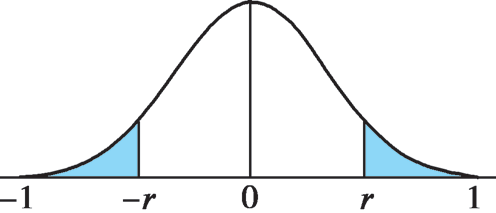
\includegraphics[width=0.25\textwidth]{image/chart11.png}
    \caption*{附表 11 图示}
\end{figure}

\begin{longtable}{c|ccccc}
    \hline
    $v$ & \multicolumn{5}{c}{概率 $P$ (双侧)} \\
    & 0.10 & 0.05 & 0.02 & 0.01 & 0.001 \\
    \hline
    \endhead
    1  & 0.988 & 0.997 & 1.000 & 1.000 & 1.000 \\
    2  & 0.900 & 0.950 & 0.980 & 0.990 & 0.999 \\
    3  & 0.805 & 0.878 & 0.934 & 0.959 & 0.991 \\
    4  & 0.729 & 0.811 & 0.882 & 0.917 & 0.974 \\
    5  & 0.669 & 0.755 & 0.833 & 0.875 & 0.951 \\
    6  & 0.621 & 0.707 & 0.789 & 0.834 & 0.925 \\
    7  & 0.582 & 0.666 & 0.750 & 0.798 & 0.898 \\
    8  & 0.549 & 0.632 & 0.715 & 0.765 & 0.872 \\
    9  & 0.521 & 0.602 & 0.685 & 0.735 & 0.847 \\
    10 & 0.497 & 0.576 & 0.658 & 0.708 & 0.823 \\
    11 & 0.476 & 0.553 & 0.634 & 0.684 & 0.801 \\
    12 & 0.457 & 0.532 & 0.612 & 0.661 & 0.780 \\
    13 & 0.441 & 0.514 & 0.592 & 0.641 & 0.760 \\
    14 & 0.426 & 0.497 & 0.574 & 0.623 & 0.742 \\
    15 & 0.412 & 0.482 & 0.558 & 0.606 & 0.725 \\
    16 & 0.400 & 0.468 & 0.542 & 0.590 & 0.708 \\
    17 & 0.389 & 0.456 & 0.529 & 0.575 & 0.693 \\
    18 & 0.378 & 0.444 & 0.515 & 0.561 & 0.679 \\
    19 & 0.369 & 0.433 & 0.503 & 0.549 & 0.665 \\
    20 & 0.360 & 0.423 & 0.492 & 0.537 & 0.652 \\
    25 & 0.323 & 0.381 & 0.445 & 0.487 & 0.597 \\
    30 & 0.296 & 0.349 & 0.409 & 0.449 & 0.554 \\
    35 & 0.275 & 0.325 & 0.381 & 0.418 & 0.519 \\
    40 & 0.257 & 0.304 & 0.358 & 0.393 & 0.490 \\
    45 & 0.243 & 0.288 & 0.338 & 0.372 & 0.465 \\
    50 & 0.231 & 0.273 & 0.322 & 0.354 & 0.443 \\
    \hline
\end{longtable}

\newpage

% ==========================================
% 附表 12 rs 界值表
% ==========================================
\section{附表 12 $r_s$ 界值表}
\begin{longtable}{c|ccccc}
    \hline
    $n$ & \multicolumn{5}{c}{概率 $P$ (双侧)} \\
    & 0.10 & 0.05 & 0.02 & 0.01 & 0.001 \\
    \hline
    \endhead
    4  & 1.000 & & & & \\
    5  & 0.900 & 1.000 & 1.000 & & \\
    6  & 0.829 & 0.886 & 0.943 & 1.000 & \\
    7  & 0.714 & 0.786 & 0.893 & 0.929 & 1.000 \\
    8  & 0.643 & 0.738 & 0.833 & 0.881 & 0.976 \\
    9  & 0.600 & 0.700 & 0.783 & 0.833 & 0.933 \\
    10 & 0.564 & 0.648 & 0.745 & 0.794 & 0.903 \\
    11 & 0.536 & 0.618 & 0.709 & 0.755 & 0.873 \\
    12 & 0.503 & 0.587 & 0.678 & 0.727 & 0.846 \\
    13 & 0.484 & 0.560 & 0.648 & 0.703 & 0.824 \\
    14 & 0.464 & 0.538 & 0.626 & 0.679 & 0.802 \\
    15 & 0.446 & 0.521 & 0.604 & 0.650 & 0.779 \\
    16 & 0.429 & 0.503 & 0.582 & 0.635 & 0.762 \\
    17 & 0.414 & 0.485 & 0.566 & 0.615 & 0.748 \\
    18 & 0.401 & 0.472 & 0.550 & 0.600 & 0.728 \\
    19 & 0.391 & 0.460 & 0.535 & 0.584 & 0.712 \\
    20 & 0.380 & 0.447 & 0.520 & 0.570 & 0.696 \\
    25 & 0.337 & 0.398 & 0.466 & 0.511 & 0.630 \\
    30 & 0.306 & 0.362 & 0.425 & 0.467 & 0.580 \\
    35 & 0.283 & 0.335 & 0.394 & 0.433 & 0.539 \\
    40 & 0.264 & 0.313 & 0.368 & 0.405 & 0.507 \\
    45 & 0.248 & 0.294 & 0.347 & 0.382 & 0.479 \\
    50 & 0.235 & 0.279 & 0.329 & 0.363 & 0.456 \\
    \hline
\end{longtable}

\newpage

% ==========================================
% 附表 13 随机数字表
% ==========================================
\section{附表 13 随机数字表}
\scriptsize
\begin{longtable}{ccccccccccccccc}
    88 56 53 27 59 & 33 35 72 67 47 & 77 34 55 45 70 & 08 18 27 38 90 & 16 95 86 70 75 \\
    09 72 95 84 29 & 49 41 31 06 70 & 42 38 06 45 18 & 64 84 73 31 65 & 52 53 37 97 15 \\
    12 96 88 17 31 & 65 19 69 02 83 & 60 75 86 90 68 & 24 64 19 35 51 & 56 61 87 39 12 \\
    85 94 57 24 16 & 92 09 84 38 76 & 22 00 27 69 85 & 29 81 94 78 10 & 21 94 47 90 12 \\
    38 64 43 59 93 & 98 77 87 68 07 & 91 51 67 62 44 & 40 98 05 93 78 & 23 32 65 41 18 \\
    53 44 09 42 72 & 00 41 86 79 79 & 68 47 22 00 20 & 35 55 31 51 51 & 00 83 63 22 55 \\
    40 76 66 26 84 & 57 99 99 90 37 & 36 63 32 08 58 & 37 40 13 68 97 & 87 64 81 07 83 \\
    02 17 79 18 05 & 12 59 52 57 02 & 22 07 90 47 03 & 28 14 11 30 79 & 20 69 22 40 98 \\
    95 17 82 06 53 & 31 51 10 96 46 & 92 06 88 07 77 & 56 11 50 81 69 & 40 23 72 51 39 \\
    35 76 22 42 92 & 96 11 83 44 80 & 34 68 35 48 77 & 33 42 40 90 60 & 73 96 53 97 86 \\
    26 29 13 56 41 & 85 47 04 66 08 & 34 72 57 59 13 & 82 43 80 46 15 & 38 26 61 70 04 \\
    77 80 20 75 82 & 72 82 32 99 90 & 63 95 73 76 63 & 89 73 44 99 05 & 48 67 26 43 18 \\
    46 40 66 44 52 & 91 36 74 43 53 & 30 82 13 54 00 & 78 45 63 98 35 & 55 03 36 67 68 \\
    37 56 08 18 09 & 77 53 84 46 47 & 31 91 18 95 58 & 24 16 74 11 53 & 44 10 13 85 57 \\
    61 65 61 68 66 & 37 27 47 39 19 & 84 83 70 07 48 & 53 21 40 06 71 & 95 06 79 88 54 \\
    93 43 69 64 07 & 34 18 04 52 35 & 56 27 09 24 86 & 61 85 53 83 45 & 19 90 70 99 00 \\
    21 96 60 12 99 & 11 20 99 45 18 & 48 13 93 55 34 & 18 37 79 49 90 & 65 97 38 20 46 \\
    95 20 47 97 97 & 27 37 83 28 71 & 00 06 41 41 74 & 45 89 09 39 84 & 51 67 11 52 49 \\
    97 86 21 78 73 & 10 65 81 92 59 & 58 76 17 14 97 & 04 76 62 16 17 & 17 95 70 45 80 \\
    62 92 06 34 13 & 59 71 74 17 32 & 27 55 10 24 19 & 23 71 82 13 74 & 63 52 52 01 41 \\
    04 31 17 21 56 & 33 73 99 19 87 & 26 72 39 27 67 & 53 77 57 68 93 & 60 61 97 22 61 \\
    61 06 98 03 91 & 87 14 77 43 96 & 43 00 65 98 50 & 45 60 33 01 07 & 98 99 46 50 47 \\
    85 93 85 86 88 & 72 87 08 62 40 & 16 06 10 89 20 & 23 21 34 74 97 & 76 38 03 29 63 \\
    21 74 32 47 45 & 73 96 07 94 52 & 09 65 90 77 47 & 25 76 16 19 33 & 53 05 70 53 30 \\
    15 69 53 82 88 & 79 96 23 53 10 & 65 39 07 16 29 & 45 33 02 43 70 & 02 87 40 41 45 \\
    02 89 08 04 49 & 20 21 14 68 86 & 87 63 93 95 17 & 11 29 01 95 80 & 35 14 97 35 33 \\
    87 18 15 89 79 & 85 43 01 72 73 & 08 61 74 51 69 & 89 74 39 82 15 & 94 51 33 41 67 \\
    98 83 71 94 22 & 59 97 50 99 52 & 08 52 85 08 40 & 87 80 61 65 31 & 91 51 80 32 44 \\
    10 08 58 21 66 & 72 68 49 29 31 & 89 85 84 46 06 & 59 73 19 85 23 & 65 09 29 75 63 \\
    47 90 56 10 08 & 88 02 84 27 83 & 42 29 72 23 19 & 66 56 45 65 79 & 20 71 53 20 25 \\
    22 85 61 68 90 & 49 64 92 85 44 & 16 40 12 89 88 & 50 14 49 81 06 & 01 82 77 45 12 \\
    67 80 43 79 33 & 12 83 11 41 16 & 25 58 19 68 70 & 77 02 54 00 52 & 53 43 37 15 26 \\
    27 62 50 96 72 & 79 44 61 40 15 & 14 53 40 65 39 & 27 31 58 50 28 & 11 39 03 34 25 \\
    33 78 80 87 15 & 38 30 06 38 21 & 14 47 47 07 26 & 54 96 87 53 32 & 40 36 40 69 76 \\
    13 13 92 66 99 & 47 24 49 57 74 & 32 25 43 62 17 & 10 97 11 69 84 & 99 63 22 32 98 \\
    10 27 53 96 23 & 71 50 54 36 23 & 54 31 04 82 98 & 04 14 12 15 09 & 26 78 25 47 47 \\
    28 41 50 61 88 & 64 85 27 20 18 & 83 36 36 05 56 & 39 71 65 09 62 & 94 76 62 11 89 \\
    34 21 42 57 02 & 59 19 18 97 48 & 80 30 03 30 98 & 05 24 67 70 07 & 84 97 50 87 46 \\
    61 81 77 23 23 & 82 82 11 54 08 & 53 28 70 58 96 & 44 07 39 55 43 & 42 34 43 39 28 \\
    61 15 18 13 54 & 16 86 20 26 88 & 90 74 80 55 09 & 14 53 90 51 17 & 52 01 63 01 59 \\
    91 76 21 64 64 & 44 91 13 32 97 & 75 31 62 66 54 & 84 80 32 75 77 & 56 08 25 70 29 \\
    00 97 79 08 06 & 37 30 28 59 85 & 53 56 68 53 40 & 01 74 39 59 73 & 30 19 99 85 48 \\
    36 46 18 34 94 & 75 20 80 27 77 & 78 91 69 16 00 & 08 43 18 73 68 & 67 69 61 34 25 \\
    88 98 99 60 50 & 65 95 79 42 94 & 93 62 40 89 96 & 43 56 47 71 66 & 46 76 29 67 02 \\
    04 37 59 87 21 & 05 02 03 24 17 & 47 97 81 56 51 & 92 34 86 01 82 & 55 51 33 12 91 \\
    63 62 06 34 41 & 94 21 78 55 09 & 72 76 45 16 94 & 29 95 81 83 83 & 79 88 01 97 30 \\
    78 47 23 53 90 & 34 41 92 45 71 & 09 23 70 70 07 & 12 38 92 79 43 & 14 85 11 47 23 \\
    87 68 62 15 43 & 53 14 36 59 25 & 54 47 33 70 15 & 59 24 48 40 35 & 50 03 42 99 36 \\
    47 60 92 10 77 & 88 59 53 11 52 & 66 25 69 07 64 & 48 68 64 71 06 & 61 65 70 22 12 \\
    56 88 87 59 41 & 65 28 04 67 53 & 95 79 88 37 31 & 50 41 06 94 76 & 81 83 17 16 33 \\
    02 57 45 86 67 & 73 43 07 34 48 & 44 26 87 93 29 & 77 09 61 67 84 & 06 69 44 77 75 \\
    31 54 14 13 17 & 48 62 11 90 60 & 68 12 93 64 28 & 46 24 79 16 76 & 14 60 25 51 01 \\
    28 50 16 43 36 & 28 97 85 58 99 & 67 22 52 76 23 & 24 70 36 54 54 & 59 28 61 71 96 \\
    63 29 62 66 50 & 02 63 45 52 38 & 67 63 47 54 75 & 83 24 78 43 20 & 92 63 13 47 48 \\
    45 65 58 26 51 & 76 96 59 38 72 & 86 57 45 71 46 & 44 67 76 14 55 & 44 88 01 62 12 \\
    39 65 36 63 70 & 77 45 85 50 51 & 74 13 39 35 22 & 30 53 36 02 95 & 49 34 88 73 61 \\
    73 71 98 16 04 & 29 18 94 51 23 & 76 51 94 84 86 & 79 93 96 38 63 & 08 58 25 58 94 \\
    72 20 56 20 11 & 72 65 71 08 86 & 79 57 95 13 91 & 97 48 72 66 48 & 09 71 17 24 89 \\
    75 17 26 99 76 & 89 37 20 70 01 & 77 31 61 95 46 & 26 97 05 73 51 & 53 33 18 72 87 \\
    37 48 60 82 29 & 81 30 15 39 14 & 48 38 75 93 29 & 06 87 37 78 48 & 45 56 00 84 47 \\
    \hline
\end{longtable}



\end{document}